\documentclass[11pt,letterpaper]{article}
% Preamble for the Fable 5.2 complete draft of 12 November 2026.
% Fonts, transcript-card box and quote macros follow the earlier project preamble
% (paper_revision_2026-11-11/integrated/preamble.tex). The fact lookup, incident
% macros and prompt box are this draft's.
\usepackage[margin=1.0in,headheight=14pt]{geometry}
\usepackage{fontspec}
\setmainfont{TeX Gyre Pagella}
\setsansfont{TeX Gyre Heros}
\setmonofont[Scale=0.85]{Latin Modern Mono}
\newfontfamily\transcriptfont{TeX Gyre Heros}[RawFeature=-tlig]
\usepackage{microtype,graphicx,booktabs,tabularx,longtable,array,amsmath,amssymb}
\usepackage{enumitem,caption,xcolor,xurl,placeins,float}
\usepackage[most]{tcolorbox}
\usepackage{needspace}
\usepackage[numbers,sort&compress]{natbib}
\usepackage[colorlinks=true,linkcolor=blue!40!black,citecolor=blue!40!black,urlcolor=blue!40!black]{hyperref}
\graphicspath{{assets/}}
\setlength{\parskip}{3.5pt plus 1pt}
\setlength{\emergencystretch}{2em}
\setlist{itemsep=2pt,topsep=4pt,leftmargin=1.6em}
\captionsetup{font=small,labelfont=bf}
\newcolumntype{Y}{>{\raggedright\arraybackslash}X}
\newcolumntype{L}[1]{>{\raggedright\arraybackslash}p{#1}}
\newcommand{\artifact}[1]{\path{#1}}
% Every number in the text is a lookup into sections/facts.tex, which
% analysis/build_tables.py writes from the analysis outputs.
\newcommand{\fact}[1]{\ifcsname fact@#1\endcsname\csname fact@#1\endcsname\else\PackageError{facts}{Undefined fact: #1}{}\fi}
% Transcript cards. Quotation text and metadata come from analysis/build_quotes.py.
\definecolor{transcriptbg}{HTML}{F4F5F6}
\definecolor{transcriptborder}{HTML}{D9DDE1}
\definecolor{transcriptmeta}{HTML}{50575E}
\newtcolorbox{transcriptmessage}{enhanced,colback=transcriptbg,
  colframe=transcriptborder,boxrule=0.45pt,arc=2.5mm,
  left=10pt,right=10pt,top=6pt,bottom=7pt,
  before skip=5pt,after skip=5pt,
  fontupper=\transcriptfont\fontsize{10}{13.2}\selectfont\raggedright,
  before upper={\hyphenpenalty=10000\exhyphenpenalty=10000}}
\newcommand{\DeclareTranscriptQuote}[3]{%
  \expandafter\gdef\csname transcript@#1\endcsname{%
    \begin{transcriptmessage}
    {\color{transcriptmeta}\fontsize{8.5}{11}\selectfont #2\par}
    \smallskip #3
    \end{transcriptmessage}}}
\newcommand{\TranscriptQuote}[1]{\ifcsname transcript@#1\endcsname\csname transcript@#1\endcsname\else\PackageError{quotes}{Undefined quote: #1}{}\fi}
\newcommand{\DeclareInlineQuote}[2]{\expandafter\gdef\csname inlinequote@#1\endcsname{#2}}
\newcommand{\InlineQuote}[1]{\ifcsname inlinequote@#1\endcsname ``{\transcriptfont\small\csname inlinequote@#1\endcsname}''\else\PackageError{quotes}{Undefined inline quote: #1}{}\fi}
\newcounter{incident}
\newcommand{\IncidentTitle}[2]{\par\addvspace{0.9em}\Needspace{8\baselineskip}%
  \refstepcounter{incident}\label{inc:#1}%
  \noindent{\large\bfseries Incident \theincident. #2}\par\smallskip}
\newcommand{\IncidentSource}[1]{\par\smallskip{\footnotesize\color{transcriptmeta}#1}\par}
\newtcolorbox{promptbox}[1][]{enhanced,breakable,colback=white,colframe=transcriptborder,boxrule=0.45pt,arc=1mm,
  left=8pt,right=8pt,top=5pt,bottom=5pt,before skip=6pt,after skip=6pt,
  fontupper=\ttfamily\fontsize{9.8}{12.2}\selectfont\raggedright,#1}

\hypersetup{pdftitle={What a Move Unlocks: Stated Consequences and Actions of LLM Agents in Twenty Monopoly Games},pdfauthor={MonopolyBench project}}
\title{What a Move Unlocks:\\Stated Consequences and Actions of LLM Agents\\in Twenty Monopoly Games}
\author{MonopolyBench project\thanks{Complete draft prepared by one LLM research assistant under the project owner's direction. Appendix~\ref{app:provenance} records the roles.}}
\date{12 November 2026}
\begin{document}
% Generated by analysis/build_tables.py. Do not edit by hand.
\expandafter\gdef\csname fact@c.notes.Gemini.empty\endcsname{20}
\expandafter\gdef\csname fact@c.notes.Gemini.prompts\endcsname{1,669}
\expandafter\gdef\csname fact@c.notes.Gemini.timeline-entries-total\endcsname{32,356}
\expandafter\gdef\csname fact@c.notes.Grok.empty\endcsname{20}
\expandafter\gdef\csname fact@c.notes.Grok.prompts\endcsname{1,663}
\expandafter\gdef\csname fact@c.notes.Grok.timeline-entries-total\endcsname{32,301}
\expandafter\gdef\csname fact@c.notes.Opus.empty\endcsname{1,108}
\expandafter\gdef\csname fact@c.notes.Opus.only-fallback-like\endcsname{286}
\expandafter\gdef\csname fact@c.notes.Opus.prompts\endcsname{1,696}
\expandafter\gdef\csname fact@c.notes.Opus.timeline-entries-total\endcsname{32,950}
\expandafter\gdef\csname fact@c.notes.Sol.empty\endcsname{20}
\expandafter\gdef\csname fact@c.notes.Sol.prompts\endcsname{1,961}
\expandafter\gdef\csname fact@c.notes.Sol.timeline-entries-total\endcsname{38,231}
\expandafter\gdef\csname fact@c.opus.action-only-attempts\endcsname{1,604}
\expandafter\gdef\csname fact@c.opus.action-only-refused\endcsname{0}
\expandafter\gdef\csname fact@c.opus.decisions-with-any-refusal\endcsname{1,605}
\expandafter\gdef\csname fact@c.opus.distinct-refusal-messages\endcsname{1}
\expandafter\gdef\csname fact@c.opus.first-attempt-refusals\endcsname{1,604}
\expandafter\gdef\csname fact@c.opus.refused-attempts\endcsname{1,605}
\expandafter\gdef\csname fact@c.resolution.Gemini.decisions\endcsname{1,669}
\expandafter\gdef\csname fact@c.resolution.Gemini.fallback-used\endcsname{1}
\expandafter\gdef\csname fact@c.resolution.Gemini.has-private-thought-applied\endcsname{1,669}
\expandafter\gdef\csname fact@c.resolution.Gemini.retry-used\endcsname{20}
\expandafter\gdef\csname fact@c.resolution.Grok.decisions\endcsname{1,663}
\expandafter\gdef\csname fact@c.resolution.Grok.fallback-used\endcsname{0}
\expandafter\gdef\csname fact@c.resolution.Grok.has-private-thought-applied\endcsname{1,663}
\expandafter\gdef\csname fact@c.resolution.Grok.retry-used\endcsname{35}
\expandafter\gdef\csname fact@c.resolution.Opus.decisions\endcsname{1,696}
\expandafter\gdef\csname fact@c.resolution.Opus.engine-default-after-action-only-attempt\endcsname{60}
\expandafter\gdef\csname fact@c.resolution.Opus.fallback-used\endcsname{61}
\expandafter\gdef\csname fact@c.resolution.Opus.has-private-thought-applied\endcsname{152}
\expandafter\gdef\csname fact@c.resolution.Opus.retry-used\endcsname{1,605}
\expandafter\gdef\csname fact@c.resolution.Sol.decisions\endcsname{1,961}
\expandafter\gdef\csname fact@c.resolution.Sol.fallback-used\endcsname{4}
\expandafter\gdef\csname fact@c.resolution.Sol.has-private-thought-applied\endcsname{1,961}
\expandafter\gdef\csname fact@c.resolution.Sol.retry-used\endcsname{30}
\expandafter\gdef\csname fact@d.above-bound.declared-at-first-menu\endcsname{50}
\expandafter\gdef\csname fact@d.above-bound.episodes\endcsname{56}
\expandafter\gdef\csname fact@d.above-bound.liquidated-before-elimination\endcsname{5}
\expandafter\gdef\csname fact@d.above-bound.termination.automatic\endcsname{3}
\expandafter\gdef\csname fact@d.above-bound.termination.declared\endcsname{53}
\expandafter\gdef\csname fact@d.by-model.Gemini.episodes\endcsname{50}
\expandafter\gdef\csname fact@d.by-model.Gemini.multi-action\endcsname{19}
\expandafter\gdef\csname fact@d.by-model.Gemini.necessary\endcsname{6}
\expandafter\gdef\csname fact@d.by-model.Gemini.necessary-paid\endcsname{5}
\expandafter\gdef\csname fact@d.by-model.Gemini.paid\endcsname{37}
\expandafter\gdef\csname fact@d.by-model.Gemini.used-unlisted\endcsname{9}
\expandafter\gdef\csname fact@d.by-model.Grok.episodes\endcsname{38}
\expandafter\gdef\csname fact@d.by-model.Grok.multi-action\endcsname{6}
\expandafter\gdef\csname fact@d.by-model.Grok.necessary\endcsname{2}
\expandafter\gdef\csname fact@d.by-model.Grok.necessary-paid\endcsname{2}
\expandafter\gdef\csname fact@d.by-model.Grok.paid\endcsname{20}
\expandafter\gdef\csname fact@d.by-model.Grok.used-unlisted\endcsname{2}
\expandafter\gdef\csname fact@d.by-model.Opus.episodes\endcsname{58}
\expandafter\gdef\csname fact@d.by-model.Opus.multi-action\endcsname{19}
\expandafter\gdef\csname fact@d.by-model.Opus.necessary\endcsname{5}
\expandafter\gdef\csname fact@d.by-model.Opus.necessary-paid\endcsname{5}
\expandafter\gdef\csname fact@d.by-model.Opus.paid\endcsname{41}
\expandafter\gdef\csname fact@d.by-model.Opus.used-unlisted\endcsname{5}
\expandafter\gdef\csname fact@d.by-model.Sol.episodes\endcsname{42}
\expandafter\gdef\csname fact@d.by-model.Sol.multi-action\endcsname{17}
\expandafter\gdef\csname fact@d.by-model.Sol.necessary\endcsname{3}
\expandafter\gdef\csname fact@d.by-model.Sol.necessary-paid\endcsname{2}
\expandafter\gdef\csname fact@d.by-model.Sol.paid\endcsname{30}
\expandafter\gdef\csname fact@d.by-model.Sol.used-unlisted\endcsname{3}
\expandafter\gdef\csname fact@d.classes.above-bound\endcsname{56}
\expandafter\gdef\csname fact@d.classes.menu-restricted\endcsname{1}
\expandafter\gdef\csname fact@d.classes.paid\endcsname{128}
\expandafter\gdef\csname fact@d.classes.payable-declared\endcsname{3}
\expandafter\gdef\csname fact@d.eliminations.nonterminal\endcsname{40}
\expandafter\gdef\csname fact@d.eliminations.nonterminal-to-eventual-winner\endcsname{35}
\expandafter\gdef\csname fact@d.eliminations.to-player-creditor\endcsname{59}
\expandafter\gdef\csname fact@d.eliminations.total\endcsname{60}
\expandafter\gdef\csname fact@d.episodes\endcsname{188}
\expandafter\gdef\csname fact@d.first-menu-decision.above-bound-continue\endcsname{6}
\expandafter\gdef\csname fact@d.first-menu-decision.above-bound-declare\endcsname{50}
\expandafter\gdef\csname fact@d.first-menu-decision.menu-restricted-continue\endcsname{1}
\expandafter\gdef\csname fact@d.first-menu-decision.payable-continue\endcsname{128}
\expandafter\gdef\csname fact@d.first-menu-decision.payable-declare\endcsname{3}
\expandafter\gdef\csname fact@d.liquidation-decisions\endcsname{338}
\expandafter\gdef\csname fact@d.necessary.blocks-with-cases\endcsname{5}
\expandafter\gdef\csname fact@d.necessary.episodes\endcsname{16}
\expandafter\gdef\csname fact@d.necessary.first-action-paid.mortgage-property\endcsname{1}
\expandafter\gdef\csname fact@d.necessary.first-action-paid.sell-houses-or-hotel\endcsname{13}
\expandafter\gdef\csname fact@d.necessary.first-action.declare-bankruptcy\endcsname{2}
\expandafter\gdef\csname fact@d.necessary.first-action.mortgage-property\endcsname{1}
\expandafter\gdef\csname fact@d.necessary.first-action.sell-houses-or-hotel\endcsname{13}
\expandafter\gdef\csname fact@d.necessary.games\endcsname{12}
\expandafter\gdef\csname fact@d.necessary.median-actions-paid\endcsname{4}
\expandafter\gdef\csname fact@d.necessary.median-cash-after-payment\endcsname{56}
\expandafter\gdef\csname fact@d.necessary.median-shortfall-without-unlisted\endcsname{83}
\expandafter\gdef\csname fact@d.necessary.paid\endcsname{14}
\expandafter\gdef\csname fact@d.paid-actions.debt-total\endcsname{51,997}
\expandafter\gdef\csname fact@d.paid-actions.fallback-in-paid\endcsname{0}
\expandafter\gdef\csname fact@d.paid-actions.max-actions\endcsname{10}
\expandafter\gdef\csname fact@d.paid-actions.median-debt-over-bound\endcsname{0.4}
\expandafter\gdef\csname fact@d.paid-actions.mortgages\endcsname{180}
\expandafter\gdef\csname fact@d.paid-actions.multi-action\endcsname{61}
\expandafter\gdef\csname fact@d.paid-actions.sales\endcsname{89}
\expandafter\gdef\csname fact@d.paid-actions.single-action\endcsname{67}
\expandafter\gdef\csname fact@d.payable\endcsname{131}
\expandafter\gdef\csname fact@d.tiers-among-payable.listed.by-block.1.0\endcsname{14}
\expandafter\gdef\csname fact@d.tiers-among-payable.listed.by-block.1.1\endcsname{14}
\expandafter\gdef\csname fact@d.tiers-among-payable.listed.by-block.2.0\endcsname{11}
\expandafter\gdef\csname fact@d.tiers-among-payable.listed.by-block.2.1\endcsname{11}
\expandafter\gdef\csname fact@d.tiers-among-payable.listed.by-block.3.0\endcsname{7}
\expandafter\gdef\csname fact@d.tiers-among-payable.listed.by-block.3.1\endcsname{7}
\expandafter\gdef\csname fact@d.tiers-among-payable.listed.by-block.4.0\endcsname{15}
\expandafter\gdef\csname fact@d.tiers-among-payable.listed.by-block.4.1\endcsname{15}
\expandafter\gdef\csname fact@d.tiers-among-payable.listed.by-block.5.0\endcsname{15}
\expandafter\gdef\csname fact@d.tiers-among-payable.listed.by-block.5.1\endcsname{15}
\expandafter\gdef\csname fact@d.tiers-among-payable.listed.by-model.Gemini.0\endcsname{16}
\expandafter\gdef\csname fact@d.tiers-among-payable.listed.by-model.Gemini.1\endcsname{16}
\expandafter\gdef\csname fact@d.tiers-among-payable.listed.by-model.Grok.0\endcsname{7}
\expandafter\gdef\csname fact@d.tiers-among-payable.listed.by-model.Grok.1\endcsname{7}
\expandafter\gdef\csname fact@d.tiers-among-payable.listed.by-model.Opus.0\endcsname{26}
\expandafter\gdef\csname fact@d.tiers-among-payable.listed.by-model.Opus.1\endcsname{26}
\expandafter\gdef\csname fact@d.tiers-among-payable.listed.by-model.Sol.0\endcsname{13}
\expandafter\gdef\csname fact@d.tiers-among-payable.listed.by-model.Sol.1\endcsname{13}
\expandafter\gdef\csname fact@d.tiers-among-payable.listed.declared\endcsname{0}
\expandafter\gdef\csname fact@d.tiers-among-payable.listed.episodes\endcsname{62}
\expandafter\gdef\csname fact@d.tiers-among-payable.listed.games\endcsname{18}
\expandafter\gdef\csname fact@d.tiers-among-payable.listed.max-actions-when-paid\endcsname{7}
\expandafter\gdef\csname fact@d.tiers-among-payable.listed.median-actions-when-paid\endcsname{1}
\expandafter\gdef\csname fact@d.tiers-among-payable.listed.median-debt\endcsname{200}
\expandafter\gdef\csname fact@d.tiers-among-payable.listed.paid\endcsname{62}
\expandafter\gdef\csname fact@d.tiers-among-payable.listed.single-action-payments\endcsname{37}
\expandafter\gdef\csname fact@d.tiers-among-payable.sales.by-block.1.0\endcsname{21}
\expandafter\gdef\csname fact@d.tiers-among-payable.sales.by-block.1.1\endcsname{21}
\expandafter\gdef\csname fact@d.tiers-among-payable.sales.by-block.2.0\endcsname{6}
\expandafter\gdef\csname fact@d.tiers-among-payable.sales.by-block.2.1\endcsname{6}
\expandafter\gdef\csname fact@d.tiers-among-payable.sales.by-block.3.0\endcsname{4}
\expandafter\gdef\csname fact@d.tiers-among-payable.sales.by-block.3.1\endcsname{5}
\expandafter\gdef\csname fact@d.tiers-among-payable.sales.by-block.4.0\endcsname{9}
\expandafter\gdef\csname fact@d.tiers-among-payable.sales.by-block.4.1\endcsname{9}
\expandafter\gdef\csname fact@d.tiers-among-payable.sales.by-block.5.0\endcsname{12}
\expandafter\gdef\csname fact@d.tiers-among-payable.sales.by-block.5.1\endcsname{12}
\expandafter\gdef\csname fact@d.tiers-among-payable.sales.by-model.Gemini.0\endcsname{16}
\expandafter\gdef\csname fact@d.tiers-among-payable.sales.by-model.Gemini.1\endcsname{16}
\expandafter\gdef\csname fact@d.tiers-among-payable.sales.by-model.Grok.0\endcsname{11}
\expandafter\gdef\csname fact@d.tiers-among-payable.sales.by-model.Grok.1\endcsname{12}
\expandafter\gdef\csname fact@d.tiers-among-payable.sales.by-model.Opus.0\endcsname{10}
\expandafter\gdef\csname fact@d.tiers-among-payable.sales.by-model.Opus.1\endcsname{10}
\expandafter\gdef\csname fact@d.tiers-among-payable.sales.by-model.Sol.0\endcsname{15}
\expandafter\gdef\csname fact@d.tiers-among-payable.sales.by-model.Sol.1\endcsname{15}
\expandafter\gdef\csname fact@d.tiers-among-payable.sales.declared\endcsname{1}
\expandafter\gdef\csname fact@d.tiers-among-payable.sales.episodes\endcsname{53}
\expandafter\gdef\csname fact@d.tiers-among-payable.sales.games\endcsname{15}
\expandafter\gdef\csname fact@d.tiers-among-payable.sales.max-actions-when-paid\endcsname{7}
\expandafter\gdef\csname fact@d.tiers-among-payable.sales.median-actions-when-paid\endcsname{1}
\expandafter\gdef\csname fact@d.tiers-among-payable.sales.median-debt\endcsname{250}
\expandafter\gdef\csname fact@d.tiers-among-payable.sales.paid\endcsname{52}
\expandafter\gdef\csname fact@d.tiers-among-payable.sales.single-action-payments\endcsname{30}
\expandafter\gdef\csname fact@d.tiers-among-payable.unlisted.by-block.1.0\endcsname{4}
\expandafter\gdef\csname fact@d.tiers-among-payable.unlisted.by-block.1.1\endcsname{4}
\expandafter\gdef\csname fact@d.tiers-among-payable.unlisted.by-block.2.0\endcsname{3}
\expandafter\gdef\csname fact@d.tiers-among-payable.unlisted.by-block.2.1\endcsname{3}
\expandafter\gdef\csname fact@d.tiers-among-payable.unlisted.by-block.3.0\endcsname{1}
\expandafter\gdef\csname fact@d.tiers-among-payable.unlisted.by-block.3.1\endcsname{2}
\expandafter\gdef\csname fact@d.tiers-among-payable.unlisted.by-block.4.0\endcsname{1}
\expandafter\gdef\csname fact@d.tiers-among-payable.unlisted.by-block.4.1\endcsname{1}
\expandafter\gdef\csname fact@d.tiers-among-payable.unlisted.by-block.5.0\endcsname{5}
\expandafter\gdef\csname fact@d.tiers-among-payable.unlisted.by-block.5.1\endcsname{6}
\expandafter\gdef\csname fact@d.tiers-among-payable.unlisted.by-model.Gemini.0\endcsname{5}
\expandafter\gdef\csname fact@d.tiers-among-payable.unlisted.by-model.Gemini.1\endcsname{6}
\expandafter\gdef\csname fact@d.tiers-among-payable.unlisted.by-model.Grok.0\endcsname{2}
\expandafter\gdef\csname fact@d.tiers-among-payable.unlisted.by-model.Grok.1\endcsname{2}
\expandafter\gdef\csname fact@d.tiers-among-payable.unlisted.by-model.Opus.0\endcsname{5}
\expandafter\gdef\csname fact@d.tiers-among-payable.unlisted.by-model.Opus.1\endcsname{5}
\expandafter\gdef\csname fact@d.tiers-among-payable.unlisted.by-model.Sol.0\endcsname{2}
\expandafter\gdef\csname fact@d.tiers-among-payable.unlisted.by-model.Sol.1\endcsname{3}
\expandafter\gdef\csname fact@d.tiers-among-payable.unlisted.declared\endcsname{2}
\expandafter\gdef\csname fact@d.tiers-among-payable.unlisted.episodes\endcsname{16}
\expandafter\gdef\csname fact@d.tiers-among-payable.unlisted.games\endcsname{12}
\expandafter\gdef\csname fact@d.tiers-among-payable.unlisted.max-actions-when-paid\endcsname{10}
\expandafter\gdef\csname fact@d.tiers-among-payable.unlisted.median-actions-when-paid\endcsname{4}
\expandafter\gdef\csname fact@d.tiers-among-payable.unlisted.median-debt\endcsname{587.5}
\expandafter\gdef\csname fact@d.tiers-among-payable.unlisted.paid\endcsname{14}
\expandafter\gdef\csname fact@d.tiers-among-payable.unlisted.single-action-payments\endcsname{0}
\expandafter\gdef\csname fact@d.unlisted-use.by-model.Gemini\endcsname{9}
\expandafter\gdef\csname fact@d.unlisted-use.by-model.Grok\endcsname{2}
\expandafter\gdef\csname fact@d.unlisted-use.by-model.Opus\endcsname{5}
\expandafter\gdef\csname fact@d.unlisted-use.by-model.Sol\endcsname{3}
\expandafter\gdef\csname fact@d.unlisted-use.episodes\endcsname{19}
\expandafter\gdef\csname fact@d.unlisted-use.mortgages\endcsname{33}
\expandafter\gdef\csname fact@d.unlisted-use.necessary\endcsname{14}
\expandafter\gdef\csname fact@d.unlisted-use.optional\endcsname{5}
\expandafter\gdef\csname fact@o.by-block.1.cash-bid-neither.accept\endcsname{2}
\expandafter\gdef\csname fact@o.by-block.1.cash-bid-neither.counter\endcsname{8}
\expandafter\gdef\csname fact@o.by-block.1.cash-bid-neither.n\endcsname{15}
\expandafter\gdef\csname fact@o.by-block.1.cash-bid-neither.reject\endcsname{5}
\expandafter\gdef\csname fact@o.by-block.1.cash-bid-proposer-only.accept\endcsname{1}
\expandafter\gdef\csname fact@o.by-block.1.cash-bid-proposer-only.counter\endcsname{7}
\expandafter\gdef\csname fact@o.by-block.1.cash-bid-proposer-only.n\endcsname{9}
\expandafter\gdef\csname fact@o.by-block.1.cash-bid-proposer-only.reject\endcsname{1}
\expandafter\gdef\csname fact@o.by-block.1.swap-neither.accept\endcsname{2}
\expandafter\gdef\csname fact@o.by-block.1.swap-neither.counter\endcsname{6}
\expandafter\gdef\csname fact@o.by-block.1.swap-neither.n\endcsname{16}
\expandafter\gdef\csname fact@o.by-block.1.swap-neither.reject\endcsname{8}
\expandafter\gdef\csname fact@o.by-block.1.swap-proposer-only.accept\endcsname{0}
\expandafter\gdef\csname fact@o.by-block.1.swap-proposer-only.counter\endcsname{5}
\expandafter\gdef\csname fact@o.by-block.1.swap-proposer-only.n\endcsname{34}
\expandafter\gdef\csname fact@o.by-block.1.swap-proposer-only.reject\endcsname{29}
\expandafter\gdef\csname fact@o.by-block.2.cash-bid-neither.accept\endcsname{1}
\expandafter\gdef\csname fact@o.by-block.2.cash-bid-neither.counter\endcsname{9}
\expandafter\gdef\csname fact@o.by-block.2.cash-bid-neither.n\endcsname{37}
\expandafter\gdef\csname fact@o.by-block.2.cash-bid-neither.reject\endcsname{27}
\expandafter\gdef\csname fact@o.by-block.2.cash-bid-proposer-only.accept\endcsname{0}
\expandafter\gdef\csname fact@o.by-block.2.cash-bid-proposer-only.counter\endcsname{3}
\expandafter\gdef\csname fact@o.by-block.2.cash-bid-proposer-only.n\endcsname{10}
\expandafter\gdef\csname fact@o.by-block.2.cash-bid-proposer-only.reject\endcsname{7}
\expandafter\gdef\csname fact@o.by-block.2.swap-neither.accept\endcsname{4}
\expandafter\gdef\csname fact@o.by-block.2.swap-neither.counter\endcsname{6}
\expandafter\gdef\csname fact@o.by-block.2.swap-neither.n\endcsname{21}
\expandafter\gdef\csname fact@o.by-block.2.swap-neither.reject\endcsname{11}
\expandafter\gdef\csname fact@o.by-block.2.swap-proposer-only.accept\endcsname{0}
\expandafter\gdef\csname fact@o.by-block.2.swap-proposer-only.counter\endcsname{1}
\expandafter\gdef\csname fact@o.by-block.2.swap-proposer-only.n\endcsname{14}
\expandafter\gdef\csname fact@o.by-block.2.swap-proposer-only.reject\endcsname{13}
\expandafter\gdef\csname fact@o.by-block.3.cash-bid-neither.accept\endcsname{0}
\expandafter\gdef\csname fact@o.by-block.3.cash-bid-neither.counter\endcsname{7}
\expandafter\gdef\csname fact@o.by-block.3.cash-bid-neither.n\endcsname{24}
\expandafter\gdef\csname fact@o.by-block.3.cash-bid-neither.reject\endcsname{17}
\expandafter\gdef\csname fact@o.by-block.3.cash-bid-proposer-only.accept\endcsname{0}
\expandafter\gdef\csname fact@o.by-block.3.cash-bid-proposer-only.counter\endcsname{4}
\expandafter\gdef\csname fact@o.by-block.3.cash-bid-proposer-only.n\endcsname{10}
\expandafter\gdef\csname fact@o.by-block.3.cash-bid-proposer-only.reject\endcsname{6}
\expandafter\gdef\csname fact@o.by-block.3.swap-neither.accept\endcsname{2}
\expandafter\gdef\csname fact@o.by-block.3.swap-neither.counter\endcsname{5}
\expandafter\gdef\csname fact@o.by-block.3.swap-neither.n\endcsname{15}
\expandafter\gdef\csname fact@o.by-block.3.swap-neither.reject\endcsname{8}
\expandafter\gdef\csname fact@o.by-block.3.swap-proposer-only.accept\endcsname{0}
\expandafter\gdef\csname fact@o.by-block.3.swap-proposer-only.counter\endcsname{4}
\expandafter\gdef\csname fact@o.by-block.3.swap-proposer-only.n\endcsname{21}
\expandafter\gdef\csname fact@o.by-block.3.swap-proposer-only.reject\endcsname{17}
\expandafter\gdef\csname fact@o.by-block.4.cash-bid-neither.accept\endcsname{0}
\expandafter\gdef\csname fact@o.by-block.4.cash-bid-neither.counter\endcsname{3}
\expandafter\gdef\csname fact@o.by-block.4.cash-bid-neither.n\endcsname{13}
\expandafter\gdef\csname fact@o.by-block.4.cash-bid-neither.reject\endcsname{10}
\expandafter\gdef\csname fact@o.by-block.4.cash-bid-proposer-only.accept\endcsname{0}
\expandafter\gdef\csname fact@o.by-block.4.cash-bid-proposer-only.counter\endcsname{6}
\expandafter\gdef\csname fact@o.by-block.4.cash-bid-proposer-only.n\endcsname{21}
\expandafter\gdef\csname fact@o.by-block.4.cash-bid-proposer-only.reject\endcsname{15}
\expandafter\gdef\csname fact@o.by-block.4.swap-neither.accept\endcsname{5}
\expandafter\gdef\csname fact@o.by-block.4.swap-neither.counter\endcsname{1}
\expandafter\gdef\csname fact@o.by-block.4.swap-neither.n\endcsname{11}
\expandafter\gdef\csname fact@o.by-block.4.swap-neither.reject\endcsname{5}
\expandafter\gdef\csname fact@o.by-block.4.swap-proposer-only.accept\endcsname{1}
\expandafter\gdef\csname fact@o.by-block.4.swap-proposer-only.counter\endcsname{3}
\expandafter\gdef\csname fact@o.by-block.4.swap-proposer-only.n\endcsname{19}
\expandafter\gdef\csname fact@o.by-block.4.swap-proposer-only.reject\endcsname{15}
\expandafter\gdef\csname fact@o.by-block.5.cash-bid-neither.accept\endcsname{1}
\expandafter\gdef\csname fact@o.by-block.5.cash-bid-neither.counter\endcsname{5}
\expandafter\gdef\csname fact@o.by-block.5.cash-bid-neither.n\endcsname{14}
\expandafter\gdef\csname fact@o.by-block.5.cash-bid-neither.reject\endcsname{8}
\expandafter\gdef\csname fact@o.by-block.5.cash-bid-proposer-only.accept\endcsname{1}
\expandafter\gdef\csname fact@o.by-block.5.cash-bid-proposer-only.counter\endcsname{6}
\expandafter\gdef\csname fact@o.by-block.5.cash-bid-proposer-only.n\endcsname{20}
\expandafter\gdef\csname fact@o.by-block.5.cash-bid-proposer-only.reject\endcsname{13}
\expandafter\gdef\csname fact@o.by-block.5.swap-neither.accept\endcsname{4}
\expandafter\gdef\csname fact@o.by-block.5.swap-neither.counter\endcsname{0}
\expandafter\gdef\csname fact@o.by-block.5.swap-neither.n\endcsname{9}
\expandafter\gdef\csname fact@o.by-block.5.swap-neither.reject\endcsname{5}
\expandafter\gdef\csname fact@o.by-block.5.swap-proposer-only.accept\endcsname{0}
\expandafter\gdef\csname fact@o.by-block.5.swap-proposer-only.counter\endcsname{7}
\expandafter\gdef\csname fact@o.by-block.5.swap-proposer-only.n\endcsname{28}
\expandafter\gdef\csname fact@o.by-block.5.swap-proposer-only.reject\endcsname{21}
\expandafter\gdef\csname fact@o.by-proposer.Gemini.cash-bid-neither.accept\endcsname{0}
\expandafter\gdef\csname fact@o.by-proposer.Gemini.cash-bid-neither.counter\endcsname{0}
\expandafter\gdef\csname fact@o.by-proposer.Gemini.cash-bid-neither.n\endcsname{0}
\expandafter\gdef\csname fact@o.by-proposer.Gemini.cash-bid-neither.reject\endcsname{0}
\expandafter\gdef\csname fact@o.by-proposer.Gemini.cash-bid-proposer-only.accept\endcsname{1}
\expandafter\gdef\csname fact@o.by-proposer.Gemini.cash-bid-proposer-only.counter\endcsname{2}
\expandafter\gdef\csname fact@o.by-proposer.Gemini.cash-bid-proposer-only.n\endcsname{4}
\expandafter\gdef\csname fact@o.by-proposer.Gemini.cash-bid-proposer-only.reject\endcsname{1}
\expandafter\gdef\csname fact@o.by-proposer.Gemini.swap-neither.accept\endcsname{1}
\expandafter\gdef\csname fact@o.by-proposer.Gemini.swap-neither.counter\endcsname{1}
\expandafter\gdef\csname fact@o.by-proposer.Gemini.swap-neither.n\endcsname{2}
\expandafter\gdef\csname fact@o.by-proposer.Gemini.swap-neither.reject\endcsname{0}
\expandafter\gdef\csname fact@o.by-proposer.Gemini.swap-proposer-only.accept\endcsname{0}
\expandafter\gdef\csname fact@o.by-proposer.Gemini.swap-proposer-only.counter\endcsname{4}
\expandafter\gdef\csname fact@o.by-proposer.Gemini.swap-proposer-only.n\endcsname{8}
\expandafter\gdef\csname fact@o.by-proposer.Gemini.swap-proposer-only.reject\endcsname{4}
\expandafter\gdef\csname fact@o.by-proposer.Grok.cash-bid-neither.accept\endcsname{3}
\expandafter\gdef\csname fact@o.by-proposer.Grok.cash-bid-neither.counter\endcsname{11}
\expandafter\gdef\csname fact@o.by-proposer.Grok.cash-bid-neither.n\endcsname{25}
\expandafter\gdef\csname fact@o.by-proposer.Grok.cash-bid-neither.reject\endcsname{11}
\expandafter\gdef\csname fact@o.by-proposer.Grok.cash-bid-proposer-only.accept\endcsname{0}
\expandafter\gdef\csname fact@o.by-proposer.Grok.cash-bid-proposer-only.counter\endcsname{7}
\expandafter\gdef\csname fact@o.by-proposer.Grok.cash-bid-proposer-only.n\endcsname{13}
\expandafter\gdef\csname fact@o.by-proposer.Grok.cash-bid-proposer-only.reject\endcsname{6}
\expandafter\gdef\csname fact@o.by-proposer.Grok.swap-neither.accept\endcsname{15}
\expandafter\gdef\csname fact@o.by-proposer.Grok.swap-neither.counter\endcsname{8}
\expandafter\gdef\csname fact@o.by-proposer.Grok.swap-neither.n\endcsname{36}
\expandafter\gdef\csname fact@o.by-proposer.Grok.swap-neither.reject\endcsname{13}
\expandafter\gdef\csname fact@o.by-proposer.Grok.swap-proposer-only.accept\endcsname{0}
\expandafter\gdef\csname fact@o.by-proposer.Grok.swap-proposer-only.counter\endcsname{3}
\expandafter\gdef\csname fact@o.by-proposer.Grok.swap-proposer-only.n\endcsname{8}
\expandafter\gdef\csname fact@o.by-proposer.Grok.swap-proposer-only.reject\endcsname{5}
\expandafter\gdef\csname fact@o.by-proposer.Opus.cash-bid-neither.accept\endcsname{1}
\expandafter\gdef\csname fact@o.by-proposer.Opus.cash-bid-neither.counter\endcsname{18}
\expandafter\gdef\csname fact@o.by-proposer.Opus.cash-bid-neither.n\endcsname{70}
\expandafter\gdef\csname fact@o.by-proposer.Opus.cash-bid-neither.reject\endcsname{51}
\expandafter\gdef\csname fact@o.by-proposer.Opus.cash-bid-proposer-only.accept\endcsname{1}
\expandafter\gdef\csname fact@o.by-proposer.Opus.cash-bid-proposer-only.counter\endcsname{12}
\expandafter\gdef\csname fact@o.by-proposer.Opus.cash-bid-proposer-only.n\endcsname{40}
\expandafter\gdef\csname fact@o.by-proposer.Opus.cash-bid-proposer-only.reject\endcsname{27}
\expandafter\gdef\csname fact@o.by-proposer.Opus.swap-neither.accept\endcsname{1}
\expandafter\gdef\csname fact@o.by-proposer.Opus.swap-neither.counter\endcsname{7}
\expandafter\gdef\csname fact@o.by-proposer.Opus.swap-neither.n\endcsname{23}
\expandafter\gdef\csname fact@o.by-proposer.Opus.swap-neither.reject\endcsname{15}
\expandafter\gdef\csname fact@o.by-proposer.Opus.swap-proposer-only.accept\endcsname{1}
\expandafter\gdef\csname fact@o.by-proposer.Opus.swap-proposer-only.counter\endcsname{7}
\expandafter\gdef\csname fact@o.by-proposer.Opus.swap-proposer-only.n\endcsname{50}
\expandafter\gdef\csname fact@o.by-proposer.Opus.swap-proposer-only.reject\endcsname{42}
\expandafter\gdef\csname fact@o.by-proposer.Sol.cash-bid-neither.accept\endcsname{0}
\expandafter\gdef\csname fact@o.by-proposer.Sol.cash-bid-neither.counter\endcsname{3}
\expandafter\gdef\csname fact@o.by-proposer.Sol.cash-bid-neither.n\endcsname{8}
\expandafter\gdef\csname fact@o.by-proposer.Sol.cash-bid-neither.reject\endcsname{5}
\expandafter\gdef\csname fact@o.by-proposer.Sol.cash-bid-proposer-only.accept\endcsname{0}
\expandafter\gdef\csname fact@o.by-proposer.Sol.cash-bid-proposer-only.counter\endcsname{5}
\expandafter\gdef\csname fact@o.by-proposer.Sol.cash-bid-proposer-only.n\endcsname{13}
\expandafter\gdef\csname fact@o.by-proposer.Sol.cash-bid-proposer-only.reject\endcsname{8}
\expandafter\gdef\csname fact@o.by-proposer.Sol.swap-neither.accept\endcsname{0}
\expandafter\gdef\csname fact@o.by-proposer.Sol.swap-neither.counter\endcsname{2}
\expandafter\gdef\csname fact@o.by-proposer.Sol.swap-neither.n\endcsname{11}
\expandafter\gdef\csname fact@o.by-proposer.Sol.swap-neither.reject\endcsname{9}
\expandafter\gdef\csname fact@o.by-proposer.Sol.swap-proposer-only.accept\endcsname{0}
\expandafter\gdef\csname fact@o.by-proposer.Sol.swap-proposer-only.counter\endcsname{6}
\expandafter\gdef\csname fact@o.by-proposer.Sol.swap-proposer-only.n\endcsname{50}
\expandafter\gdef\csname fact@o.by-proposer.Sol.swap-proposer-only.reject\endcsname{44}
\expandafter\gdef\csname fact@o.by-recipient.Gemini.cash-bid-neither.accept\endcsname{2}
\expandafter\gdef\csname fact@o.by-recipient.Gemini.cash-bid-neither.counter\endcsname{2}
\expandafter\gdef\csname fact@o.by-recipient.Gemini.cash-bid-neither.n\endcsname{38}
\expandafter\gdef\csname fact@o.by-recipient.Gemini.cash-bid-neither.reject\endcsname{34}
\expandafter\gdef\csname fact@o.by-recipient.Gemini.cash-bid-proposer-only.accept\endcsname{0}
\expandafter\gdef\csname fact@o.by-recipient.Gemini.cash-bid-proposer-only.counter\endcsname{1}
\expandafter\gdef\csname fact@o.by-recipient.Gemini.cash-bid-proposer-only.n\endcsname{18}
\expandafter\gdef\csname fact@o.by-recipient.Gemini.cash-bid-proposer-only.reject\endcsname{17}
\expandafter\gdef\csname fact@o.by-recipient.Gemini.swap-neither.accept\endcsname{6}
\expandafter\gdef\csname fact@o.by-recipient.Gemini.swap-neither.counter\endcsname{2}
\expandafter\gdef\csname fact@o.by-recipient.Gemini.swap-neither.n\endcsname{33}
\expandafter\gdef\csname fact@o.by-recipient.Gemini.swap-neither.reject\endcsname{25}
\expandafter\gdef\csname fact@o.by-recipient.Gemini.swap-proposer-only.accept\endcsname{0}
\expandafter\gdef\csname fact@o.by-recipient.Gemini.swap-proposer-only.counter\endcsname{4}
\expandafter\gdef\csname fact@o.by-recipient.Gemini.swap-proposer-only.n\endcsname{49}
\expandafter\gdef\csname fact@o.by-recipient.Gemini.swap-proposer-only.reject\endcsname{45}
\expandafter\gdef\csname fact@o.by-recipient.Grok.cash-bid-neither.accept\endcsname{1}
\expandafter\gdef\csname fact@o.by-recipient.Grok.cash-bid-neither.counter\endcsname{6}
\expandafter\gdef\csname fact@o.by-recipient.Grok.cash-bid-neither.n\endcsname{34}
\expandafter\gdef\csname fact@o.by-recipient.Grok.cash-bid-neither.reject\endcsname{27}
\expandafter\gdef\csname fact@o.by-recipient.Grok.cash-bid-proposer-only.accept\endcsname{2}
\expandafter\gdef\csname fact@o.by-recipient.Grok.cash-bid-proposer-only.counter\endcsname{3}
\expandafter\gdef\csname fact@o.by-recipient.Grok.cash-bid-proposer-only.n\endcsname{24}
\expandafter\gdef\csname fact@o.by-recipient.Grok.cash-bid-proposer-only.reject\endcsname{19}
\expandafter\gdef\csname fact@o.by-recipient.Grok.swap-neither.accept\endcsname{0}
\expandafter\gdef\csname fact@o.by-recipient.Grok.swap-neither.counter\endcsname{3}
\expandafter\gdef\csname fact@o.by-recipient.Grok.swap-neither.n\endcsname{12}
\expandafter\gdef\csname fact@o.by-recipient.Grok.swap-neither.reject\endcsname{9}
\expandafter\gdef\csname fact@o.by-recipient.Grok.swap-proposer-only.accept\endcsname{1}
\expandafter\gdef\csname fact@o.by-recipient.Grok.swap-proposer-only.counter\endcsname{1}
\expandafter\gdef\csname fact@o.by-recipient.Grok.swap-proposer-only.n\endcsname{37}
\expandafter\gdef\csname fact@o.by-recipient.Grok.swap-proposer-only.reject\endcsname{35}
\expandafter\gdef\csname fact@o.by-recipient.Opus.cash-bid-neither.accept\endcsname{0}
\expandafter\gdef\csname fact@o.by-recipient.Opus.cash-bid-neither.counter\endcsname{5}
\expandafter\gdef\csname fact@o.by-recipient.Opus.cash-bid-neither.n\endcsname{5}
\expandafter\gdef\csname fact@o.by-recipient.Opus.cash-bid-neither.reject\endcsname{0}
\expandafter\gdef\csname fact@o.by-recipient.Opus.cash-bid-proposer-only.accept\endcsname{0}
\expandafter\gdef\csname fact@o.by-recipient.Opus.cash-bid-proposer-only.counter\endcsname{9}
\expandafter\gdef\csname fact@o.by-recipient.Opus.cash-bid-proposer-only.n\endcsname{9}
\expandafter\gdef\csname fact@o.by-recipient.Opus.cash-bid-proposer-only.reject\endcsname{0}
\expandafter\gdef\csname fact@o.by-recipient.Opus.swap-neither.accept\endcsname{4}
\expandafter\gdef\csname fact@o.by-recipient.Opus.swap-neither.counter\endcsname{5}
\expandafter\gdef\csname fact@o.by-recipient.Opus.swap-neither.n\endcsname{11}
\expandafter\gdef\csname fact@o.by-recipient.Opus.swap-neither.reject\endcsname{2}
\expandafter\gdef\csname fact@o.by-recipient.Opus.swap-proposer-only.accept\endcsname{0}
\expandafter\gdef\csname fact@o.by-recipient.Opus.swap-proposer-only.counter\endcsname{6}
\expandafter\gdef\csname fact@o.by-recipient.Opus.swap-proposer-only.n\endcsname{9}
\expandafter\gdef\csname fact@o.by-recipient.Opus.swap-proposer-only.reject\endcsname{3}
\expandafter\gdef\csname fact@o.by-recipient.Sol.cash-bid-neither.accept\endcsname{1}
\expandafter\gdef\csname fact@o.by-recipient.Sol.cash-bid-neither.counter\endcsname{19}
\expandafter\gdef\csname fact@o.by-recipient.Sol.cash-bid-neither.n\endcsname{26}
\expandafter\gdef\csname fact@o.by-recipient.Sol.cash-bid-neither.reject\endcsname{6}
\expandafter\gdef\csname fact@o.by-recipient.Sol.cash-bid-proposer-only.accept\endcsname{0}
\expandafter\gdef\csname fact@o.by-recipient.Sol.cash-bid-proposer-only.counter\endcsname{13}
\expandafter\gdef\csname fact@o.by-recipient.Sol.cash-bid-proposer-only.n\endcsname{19}
\expandafter\gdef\csname fact@o.by-recipient.Sol.cash-bid-proposer-only.reject\endcsname{6}
\expandafter\gdef\csname fact@o.by-recipient.Sol.swap-neither.accept\endcsname{7}
\expandafter\gdef\csname fact@o.by-recipient.Sol.swap-neither.counter\endcsname{8}
\expandafter\gdef\csname fact@o.by-recipient.Sol.swap-neither.n\endcsname{16}
\expandafter\gdef\csname fact@o.by-recipient.Sol.swap-neither.reject\endcsname{1}
\expandafter\gdef\csname fact@o.by-recipient.Sol.swap-proposer-only.accept\endcsname{0}
\expandafter\gdef\csname fact@o.by-recipient.Sol.swap-proposer-only.counter\endcsname{9}
\expandafter\gdef\csname fact@o.by-recipient.Sol.swap-proposer-only.n\endcsname{21}
\expandafter\gdef\csname fact@o.by-recipient.Sol.swap-proposer-only.reject\endcsname{12}
\expandafter\gdef\csname fact@o.census.acceptance-legal\endcsname{918}
\expandafter\gdef\csname fact@o.census.by-author.Gemini.accept\endcsname{10}
\expandafter\gdef\csname fact@o.census.by-author.Gemini.counter\endcsname{37}
\expandafter\gdef\csname fact@o.census.by-author.Gemini.n\endcsname{54}
\expandafter\gdef\csname fact@o.census.by-author.Gemini.reject\endcsname{7}
\expandafter\gdef\csname fact@o.census.by-author.Grok.accept\endcsname{32}
\expandafter\gdef\csname fact@o.census.by-author.Grok.counter\endcsname{100}
\expandafter\gdef\csname fact@o.census.by-author.Grok.n\endcsname{213}
\expandafter\gdef\csname fact@o.census.by-author.Grok.reject\endcsname{81}
\expandafter\gdef\csname fact@o.census.by-author.Opus.accept\endcsname{41}
\expandafter\gdef\csname fact@o.census.by-author.Opus.counter\endcsname{136}
\expandafter\gdef\csname fact@o.census.by-author.Opus.n\endcsname{381}
\expandafter\gdef\csname fact@o.census.by-author.Opus.reject\endcsname{204}
\expandafter\gdef\csname fact@o.census.by-author.Sol.accept\endcsname{30}
\expandafter\gdef\csname fact@o.census.by-author.Sol.counter\endcsname{121}
\expandafter\gdef\csname fact@o.census.by-author.Sol.n\endcsname{272}
\expandafter\gdef\csname fact@o.census.by-author.Sol.reject\endcsname{121}
\expandafter\gdef\csname fact@o.census.by-recipient.Gemini.accept\endcsname{26}
\expandafter\gdef\csname fact@o.census.by-recipient.Gemini.counter\endcsname{36}
\expandafter\gdef\csname fact@o.census.by-recipient.Gemini.n\endcsname{242}
\expandafter\gdef\csname fact@o.census.by-recipient.Gemini.reject\endcsname{180}
\expandafter\gdef\csname fact@o.census.by-recipient.Grok.accept\endcsname{28}
\expandafter\gdef\csname fact@o.census.by-recipient.Grok.counter\endcsname{77}
\expandafter\gdef\csname fact@o.census.by-recipient.Grok.n\endcsname{254}
\expandafter\gdef\csname fact@o.census.by-recipient.Grok.reject\endcsname{149}
\expandafter\gdef\csname fact@o.census.by-recipient.Opus.accept\endcsname{29}
\expandafter\gdef\csname fact@o.census.by-recipient.Opus.counter\endcsname{141}
\expandafter\gdef\csname fact@o.census.by-recipient.Opus.n\endcsname{189}
\expandafter\gdef\csname fact@o.census.by-recipient.Opus.reject\endcsname{19}
\expandafter\gdef\csname fact@o.census.by-recipient.Sol.accept\endcsname{30}
\expandafter\gdef\csname fact@o.census.by-recipient.Sol.counter\endcsname{140}
\expandafter\gdef\csname fact@o.census.by-recipient.Sol.n\endcsname{235}
\expandafter\gdef\csname fact@o.census.by-recipient.Sol.reject\endcsname{65}
\expandafter\gdef\csname fact@o.census.grok-acceptances\endcsname{28}
\expandafter\gdef\csname fact@o.census.grok-conflicts-all\endcsname{139}
\expandafter\gdef\csname fact@o.census.grok-content-names-action\endcsname{1,068}
\expandafter\gdef\csname fact@o.census.grok-decisions\endcsname{1,663}
\expandafter\gdef\csname fact@o.census.grok-openings\endcsname{136}
\expandafter\gdef\csname fact@o.census.grok-openings-conflict\endcsname{64}
\expandafter\gdef\csname fact@o.census.grok-recipient-conflicts.accept-trade\endcsname{7}
\expandafter\gdef\csname fact@o.census.grok-recipient-conflicts.counter-trade\endcsname{1}
\expandafter\gdef\csname fact@o.census.grok-recipient-conflicts.reject-trade\endcsname{3}
\expandafter\gdef\csname fact@o.census.later\endcsname{394}
\expandafter\gdef\csname fact@o.census.opening\endcsname{524}
\expandafter\gdef\csname fact@o.census.opus-recipient-action-only\endcsname{162}
\expandafter\gdef\csname fact@o.census.other-systems-conflicts\endcsname{0}
\expandafter\gdef\csname fact@o.census.responses.accept\endcsname{113}
\expandafter\gdef\csname fact@o.census.responses.counter\endcsname{394}
\expandafter\gdef\csname fact@o.census.responses.n\endcsname{920}
\expandafter\gdef\csname fact@o.census.responses.reject\endcsname{413}
\expandafter\gdef\csname fact@o.census.threads\endcsname{526}
\expandafter\gdef\csname fact@o.composition.accepted-openings-net-list-value-to-recipient.grok-authored.0\endcsname{4,700}
\expandafter\gdef\csname fact@o.composition.accepted-openings-net-list-value-to-recipient.grok-authored.1\endcsname{21}
\expandafter\gdef\csname fact@o.composition.accepted-openings-net-list-value-to-recipient.other-authors.0\endcsname{340}
\expandafter\gdef\csname fact@o.composition.accepted-openings-net-list-value-to-recipient.other-authors.1\endcsname{11}
\expandafter\gdef\csname fact@o.composition.cash-bids-in-headline-cells\endcsname{173}
\expandafter\gdef\csname fact@o.composition.cash-bids-in-headline-cells-by-opus\endcsname{110}
\expandafter\gdef\csname fact@o.composition.conflict-opened-threads\endcsname{63}
\expandafter\gdef\csname fact@o.composition.standardized-swap-gap-pp.weights-neither-cell\endcsname{21.5}
\expandafter\gdef\csname fact@o.composition.standardized-swap-gap-pp.weights-pooled\endcsname{18.1}
\expandafter\gdef\csname fact@o.composition.standardized-swap-gap-pp.weights-proposer-only-cell\endcsname{16.0}
\expandafter\gdef\csname fact@o.composition.swap-neither-accepted\endcsname{17}
\expandafter\gdef\csname fact@o.composition.swap-neither-accepted-by-grok\endcsname{15}
\expandafter\gdef\csname fact@o.composition.swap-neither-accepted-conflict-openings\endcsname{13}
\expandafter\gdef\csname fact@o.composition.swap-neither-by-grok\endcsname{36}
\expandafter\gdef\csname fact@o.composition.swap-neither-grok-conflict-openings\endcsname{29}
\expandafter\gdef\csname fact@o.composition.without-conflict-openings.cash-bid-neither.0\endcsname{65}
\expandafter\gdef\csname fact@o.composition.without-conflict-openings.cash-bid-neither.1\endcsname{99}
\expandafter\gdef\csname fact@o.composition.without-conflict-openings.cash-bid-proposer-only.0\endcsname{40}
\expandafter\gdef\csname fact@o.composition.without-conflict-openings.cash-bid-proposer-only.1\endcsname{65}
\expandafter\gdef\csname fact@o.composition.without-conflict-openings.swap-neither.0\endcsname{26}
\expandafter\gdef\csname fact@o.composition.without-conflict-openings.swap-neither.1\endcsname{43}
\expandafter\gdef\csname fact@o.composition.without-conflict-openings.swap-proposer-only.0\endcsname{93}
\expandafter\gdef\csname fact@o.composition.without-conflict-openings.swap-proposer-only.1\endcsname{112}
\expandafter\gdef\csname fact@o.composition.without-grok-authors.cash-bid-neither.0\endcsname{56}
\expandafter\gdef\csname fact@o.composition.without-grok-authors.cash-bid-neither.1\endcsname{78}
\expandafter\gdef\csname fact@o.composition.without-grok-authors.cash-bid-proposer-only.0\endcsname{36}
\expandafter\gdef\csname fact@o.composition.without-grok-authors.cash-bid-proposer-only.1\endcsname{57}
\expandafter\gdef\csname fact@o.composition.without-grok-authors.swap-neither.0\endcsname{24}
\expandafter\gdef\csname fact@o.composition.without-grok-authors.swap-neither.1\endcsname{36}
\expandafter\gdef\csname fact@o.composition.without-grok-authors.swap-proposer-only.0\endcsname{90}
\expandafter\gdef\csname fact@o.composition.without-grok-authors.swap-proposer-only.1\endcsname{108}
\expandafter\gdef\csname fact@o.counters.all-author-only.changed-bundle\endcsname{32}
\expandafter\gdef\csname fact@o.counters.all-author-only.counters\endcsname{111}
\expandafter\gdef\csname fact@o.counters.all-author-only.same-bundle-more-cash\endcsname{79}
\expandafter\gdef\csname fact@o.counters.all-neither-deed-requests.changed-bundle\endcsname{29}
\expandafter\gdef\csname fact@o.counters.all-neither-deed-requests.counters\endcsname{110}
\expandafter\gdef\csname fact@o.counters.all-neither-deed-requests.same-bundle-more-cash\endcsname{81}
\expandafter\gdef\csname fact@o.counters.opening-cash-bid-neither.changed-bundle\endcsname{9}
\expandafter\gdef\csname fact@o.counters.opening-cash-bid-neither.counters\endcsname{32}
\expandafter\gdef\csname fact@o.counters.opening-cash-bid-neither.same-bundle-more-cash\endcsname{23}
\expandafter\gdef\csname fact@o.counters.opening-cash-bid-proposer-only.changed-bundle\endcsname{11}
\expandafter\gdef\csname fact@o.counters.opening-cash-bid-proposer-only.counters\endcsname{26}
\expandafter\gdef\csname fact@o.counters.opening-cash-bid-proposer-only.same-bundle-more-cash\endcsname{15}
\expandafter\gdef\csname fact@o.counters.opening-swap-neither.changed-bundle\endcsname{8}
\expandafter\gdef\csname fact@o.counters.opening-swap-neither.counters\endcsname{18}
\expandafter\gdef\csname fact@o.counters.opening-swap-neither.same-bundle-more-cash\endcsname{10}
\expandafter\gdef\csname fact@o.counters.opening-swap-proposer-only.changed-bundle\endcsname{10}
\expandafter\gdef\csname fact@o.counters.opening-swap-proposer-only.counters\endcsname{20}
\expandafter\gdef\csname fact@o.counters.opening-swap-proposer-only.same-bundle-more-cash\endcsname{10}
\expandafter\gdef\csname fact@o.full-table.all.all-forms.author-only.accept\endcsname{19}
\expandafter\gdef\csname fact@o.full-table.all.all-forms.author-only.counter\endcsname{111}
\expandafter\gdef\csname fact@o.full-table.all.all-forms.author-only.n\endcsname{289}
\expandafter\gdef\csname fact@o.full-table.all.all-forms.author-only.reject\endcsname{159}
\expandafter\gdef\csname fact@o.full-table.all.all-forms.both.accept\endcsname{10}
\expandafter\gdef\csname fact@o.full-table.all.all-forms.both.counter\endcsname{35}
\expandafter\gdef\csname fact@o.full-table.all.all-forms.both.n\endcsname{81}
\expandafter\gdef\csname fact@o.full-table.all.all-forms.both.reject\endcsname{36}
\expandafter\gdef\csname fact@o.full-table.all.all-forms.neither.accept\endcsname{60}
\expandafter\gdef\csname fact@o.full-table.all.all-forms.neither.counter\endcsname{169}
\expandafter\gdef\csname fact@o.full-table.all.all-forms.neither.n\endcsname{408}
\expandafter\gdef\csname fact@o.full-table.all.all-forms.neither.reject\endcsname{179}
\expandafter\gdef\csname fact@o.full-table.all.all-forms.recipient-only.accept\endcsname{24}
\expandafter\gdef\csname fact@o.full-table.all.all-forms.recipient-only.counter\endcsname{78}
\expandafter\gdef\csname fact@o.full-table.all.all-forms.recipient-only.n\endcsname{140}
\expandafter\gdef\csname fact@o.full-table.all.all-forms.recipient-only.reject\endcsname{38}
\expandafter\gdef\csname fact@o.full-table.all.cash-bid.author-only.accept\endcsname{11}
\expandafter\gdef\csname fact@o.full-table.all.cash-bid.author-only.counter\endcsname{65}
\expandafter\gdef\csname fact@o.full-table.all.cash-bid.author-only.n\endcsname{131}
\expandafter\gdef\csname fact@o.full-table.all.cash-bid.author-only.reject\endcsname{55}
\expandafter\gdef\csname fact@o.full-table.all.cash-bid.both.accept\endcsname{0}
\expandafter\gdef\csname fact@o.full-table.all.cash-bid.both.counter\endcsname{0}
\expandafter\gdef\csname fact@o.full-table.all.cash-bid.both.n\endcsname{0}
\expandafter\gdef\csname fact@o.full-table.all.cash-bid.both.reject\endcsname{0}
\expandafter\gdef\csname fact@o.full-table.all.cash-bid.neither.accept\endcsname{21}
\expandafter\gdef\csname fact@o.full-table.all.cash-bid.neither.counter\endcsname{75}
\expandafter\gdef\csname fact@o.full-table.all.cash-bid.neither.n\endcsname{176}
\expandafter\gdef\csname fact@o.full-table.all.cash-bid.neither.reject\endcsname{80}
\expandafter\gdef\csname fact@o.full-table.all.cash-bid.recipient-only.accept\endcsname{0}
\expandafter\gdef\csname fact@o.full-table.all.cash-bid.recipient-only.counter\endcsname{0}
\expandafter\gdef\csname fact@o.full-table.all.cash-bid.recipient-only.n\endcsname{0}
\expandafter\gdef\csname fact@o.full-table.all.cash-bid.recipient-only.reject\endcsname{0}
\expandafter\gdef\csname fact@o.full-table.all.form-totals.cash-bid.accept\endcsname{32}
\expandafter\gdef\csname fact@o.full-table.all.form-totals.cash-bid.counter\endcsname{140}
\expandafter\gdef\csname fact@o.full-table.all.form-totals.cash-bid.n\endcsname{307}
\expandafter\gdef\csname fact@o.full-table.all.form-totals.cash-bid.reject\endcsname{135}
\expandafter\gdef\csname fact@o.full-table.all.form-totals.other.accept\endcsname{2}
\expandafter\gdef\csname fact@o.full-table.all.form-totals.other.counter\endcsname{8}
\expandafter\gdef\csname fact@o.full-table.all.form-totals.other.n\endcsname{22}
\expandafter\gdef\csname fact@o.full-table.all.form-totals.other.reject\endcsname{12}
\expandafter\gdef\csname fact@o.full-table.all.form-totals.sale-offer.accept\endcsname{21}
\expandafter\gdef\csname fact@o.full-table.all.form-totals.sale-offer.counter\endcsname{100}
\expandafter\gdef\csname fact@o.full-table.all.form-totals.sale-offer.n\endcsname{200}
\expandafter\gdef\csname fact@o.full-table.all.form-totals.sale-offer.reject\endcsname{79}
\expandafter\gdef\csname fact@o.full-table.all.form-totals.swap.accept\endcsname{58}
\expandafter\gdef\csname fact@o.full-table.all.form-totals.swap.counter\endcsname{145}
\expandafter\gdef\csname fact@o.full-table.all.form-totals.swap.n\endcsname{389}
\expandafter\gdef\csname fact@o.full-table.all.form-totals.swap.reject\endcsname{186}
\expandafter\gdef\csname fact@o.full-table.all.other.author-only.accept\endcsname{0}
\expandafter\gdef\csname fact@o.full-table.all.other.author-only.counter\endcsname{2}
\expandafter\gdef\csname fact@o.full-table.all.other.author-only.n\endcsname{3}
\expandafter\gdef\csname fact@o.full-table.all.other.author-only.reject\endcsname{1}
\expandafter\gdef\csname fact@o.full-table.all.other.both.accept\endcsname{0}
\expandafter\gdef\csname fact@o.full-table.all.other.both.counter\endcsname{0}
\expandafter\gdef\csname fact@o.full-table.all.other.both.n\endcsname{0}
\expandafter\gdef\csname fact@o.full-table.all.other.both.reject\endcsname{0}
\expandafter\gdef\csname fact@o.full-table.all.other.neither.accept\endcsname{1}
\expandafter\gdef\csname fact@o.full-table.all.other.neither.counter\endcsname{4}
\expandafter\gdef\csname fact@o.full-table.all.other.neither.n\endcsname{13}
\expandafter\gdef\csname fact@o.full-table.all.other.neither.reject\endcsname{8}
\expandafter\gdef\csname fact@o.full-table.all.other.recipient-only.accept\endcsname{1}
\expandafter\gdef\csname fact@o.full-table.all.other.recipient-only.counter\endcsname{2}
\expandafter\gdef\csname fact@o.full-table.all.other.recipient-only.n\endcsname{6}
\expandafter\gdef\csname fact@o.full-table.all.other.recipient-only.reject\endcsname{3}
\expandafter\gdef\csname fact@o.full-table.all.sale-offer.author-only.accept\endcsname{0}
\expandafter\gdef\csname fact@o.full-table.all.sale-offer.author-only.counter\endcsname{0}
\expandafter\gdef\csname fact@o.full-table.all.sale-offer.author-only.n\endcsname{0}
\expandafter\gdef\csname fact@o.full-table.all.sale-offer.author-only.reject\endcsname{0}
\expandafter\gdef\csname fact@o.full-table.all.sale-offer.both.accept\endcsname{0}
\expandafter\gdef\csname fact@o.full-table.all.sale-offer.both.counter\endcsname{0}
\expandafter\gdef\csname fact@o.full-table.all.sale-offer.both.n\endcsname{0}
\expandafter\gdef\csname fact@o.full-table.all.sale-offer.both.reject\endcsname{0}
\expandafter\gdef\csname fact@o.full-table.all.sale-offer.neither.accept\endcsname{10}
\expandafter\gdef\csname fact@o.full-table.all.sale-offer.neither.counter\endcsname{56}
\expandafter\gdef\csname fact@o.full-table.all.sale-offer.neither.n\endcsname{113}
\expandafter\gdef\csname fact@o.full-table.all.sale-offer.neither.reject\endcsname{47}
\expandafter\gdef\csname fact@o.full-table.all.sale-offer.recipient-only.accept\endcsname{11}
\expandafter\gdef\csname fact@o.full-table.all.sale-offer.recipient-only.counter\endcsname{44}
\expandafter\gdef\csname fact@o.full-table.all.sale-offer.recipient-only.n\endcsname{87}
\expandafter\gdef\csname fact@o.full-table.all.sale-offer.recipient-only.reject\endcsname{32}
\expandafter\gdef\csname fact@o.full-table.all.swap.author-only.accept\endcsname{8}
\expandafter\gdef\csname fact@o.full-table.all.swap.author-only.counter\endcsname{44}
\expandafter\gdef\csname fact@o.full-table.all.swap.author-only.n\endcsname{155}
\expandafter\gdef\csname fact@o.full-table.all.swap.author-only.reject\endcsname{103}
\expandafter\gdef\csname fact@o.full-table.all.swap.both.accept\endcsname{10}
\expandafter\gdef\csname fact@o.full-table.all.swap.both.counter\endcsname{35}
\expandafter\gdef\csname fact@o.full-table.all.swap.both.n\endcsname{81}
\expandafter\gdef\csname fact@o.full-table.all.swap.both.reject\endcsname{36}
\expandafter\gdef\csname fact@o.full-table.all.swap.neither.accept\endcsname{28}
\expandafter\gdef\csname fact@o.full-table.all.swap.neither.counter\endcsname{34}
\expandafter\gdef\csname fact@o.full-table.all.swap.neither.n\endcsname{106}
\expandafter\gdef\csname fact@o.full-table.all.swap.neither.reject\endcsname{44}
\expandafter\gdef\csname fact@o.full-table.all.swap.recipient-only.accept\endcsname{12}
\expandafter\gdef\csname fact@o.full-table.all.swap.recipient-only.counter\endcsname{32}
\expandafter\gdef\csname fact@o.full-table.all.swap.recipient-only.n\endcsname{47}
\expandafter\gdef\csname fact@o.full-table.all.swap.recipient-only.reject\endcsname{3}
\expandafter\gdef\csname fact@o.full-table.later.all-forms.author-only.accept\endcsname{16}
\expandafter\gdef\csname fact@o.full-table.later.all-forms.author-only.counter\endcsname{65}
\expandafter\gdef\csname fact@o.full-table.later.all-forms.author-only.n\endcsname{102}
\expandafter\gdef\csname fact@o.full-table.later.all-forms.author-only.reject\endcsname{21}
\expandafter\gdef\csname fact@o.full-table.later.all-forms.both.accept\endcsname{7}
\expandafter\gdef\csname fact@o.full-table.later.all-forms.both.counter\endcsname{24}
\expandafter\gdef\csname fact@o.full-table.later.all-forms.both.n\endcsname{33}
\expandafter\gdef\csname fact@o.full-table.later.all-forms.both.reject\endcsname{2}
\expandafter\gdef\csname fact@o.full-table.later.all-forms.neither.accept\endcsname{36}
\expandafter\gdef\csname fact@o.full-table.later.all-forms.neither.counter\endcsname{107}
\expandafter\gdef\csname fact@o.full-table.later.all-forms.neither.n\endcsname{170}
\expandafter\gdef\csname fact@o.full-table.later.all-forms.neither.reject\endcsname{27}
\expandafter\gdef\csname fact@o.full-table.later.all-forms.recipient-only.accept\endcsname{22}
\expandafter\gdef\csname fact@o.full-table.later.all-forms.recipient-only.counter\endcsname{60}
\expandafter\gdef\csname fact@o.full-table.later.all-forms.recipient-only.n\endcsname{89}
\expandafter\gdef\csname fact@o.full-table.later.all-forms.recipient-only.reject\endcsname{7}
\expandafter\gdef\csname fact@o.full-table.later.cash-bid.author-only.accept\endcsname{9}
\expandafter\gdef\csname fact@o.full-table.later.cash-bid.author-only.counter\endcsname{39}
\expandafter\gdef\csname fact@o.full-table.later.cash-bid.author-only.n\endcsname{61}
\expandafter\gdef\csname fact@o.full-table.later.cash-bid.author-only.reject\endcsname{13}
\expandafter\gdef\csname fact@o.full-table.later.cash-bid.both.accept\endcsname{0}
\expandafter\gdef\csname fact@o.full-table.later.cash-bid.both.counter\endcsname{0}
\expandafter\gdef\csname fact@o.full-table.later.cash-bid.both.n\endcsname{0}
\expandafter\gdef\csname fact@o.full-table.later.cash-bid.both.reject\endcsname{0}
\expandafter\gdef\csname fact@o.full-table.later.cash-bid.neither.accept\endcsname{17}
\expandafter\gdef\csname fact@o.full-table.later.cash-bid.neither.counter\endcsname{43}
\expandafter\gdef\csname fact@o.full-table.later.cash-bid.neither.n\endcsname{73}
\expandafter\gdef\csname fact@o.full-table.later.cash-bid.neither.reject\endcsname{13}
\expandafter\gdef\csname fact@o.full-table.later.cash-bid.recipient-only.accept\endcsname{0}
\expandafter\gdef\csname fact@o.full-table.later.cash-bid.recipient-only.counter\endcsname{0}
\expandafter\gdef\csname fact@o.full-table.later.cash-bid.recipient-only.n\endcsname{0}
\expandafter\gdef\csname fact@o.full-table.later.cash-bid.recipient-only.reject\endcsname{0}
\expandafter\gdef\csname fact@o.full-table.later.form-totals.cash-bid.accept\endcsname{26}
\expandafter\gdef\csname fact@o.full-table.later.form-totals.cash-bid.counter\endcsname{82}
\expandafter\gdef\csname fact@o.full-table.later.form-totals.cash-bid.n\endcsname{134}
\expandafter\gdef\csname fact@o.full-table.later.form-totals.cash-bid.reject\endcsname{26}
\expandafter\gdef\csname fact@o.full-table.later.form-totals.other.accept\endcsname{2}
\expandafter\gdef\csname fact@o.full-table.later.form-totals.other.counter\endcsname{7}
\expandafter\gdef\csname fact@o.full-table.later.form-totals.other.n\endcsname{9}
\expandafter\gdef\csname fact@o.full-table.later.form-totals.other.reject\endcsname{0}
\expandafter\gdef\csname fact@o.full-table.later.form-totals.sale-offer.accept\endcsname{17}
\expandafter\gdef\csname fact@o.full-table.later.form-totals.sale-offer.counter\endcsname{74}
\expandafter\gdef\csname fact@o.full-table.later.form-totals.sale-offer.n\endcsname{104}
\expandafter\gdef\csname fact@o.full-table.later.form-totals.sale-offer.reject\endcsname{13}
\expandafter\gdef\csname fact@o.full-table.later.form-totals.swap.accept\endcsname{36}
\expandafter\gdef\csname fact@o.full-table.later.form-totals.swap.counter\endcsname{93}
\expandafter\gdef\csname fact@o.full-table.later.form-totals.swap.n\endcsname{147}
\expandafter\gdef\csname fact@o.full-table.later.form-totals.swap.reject\endcsname{18}
\expandafter\gdef\csname fact@o.full-table.later.other.author-only.accept\endcsname{0}
\expandafter\gdef\csname fact@o.full-table.later.other.author-only.counter\endcsname{2}
\expandafter\gdef\csname fact@o.full-table.later.other.author-only.n\endcsname{2}
\expandafter\gdef\csname fact@o.full-table.later.other.author-only.reject\endcsname{0}
\expandafter\gdef\csname fact@o.full-table.later.other.both.accept\endcsname{0}
\expandafter\gdef\csname fact@o.full-table.later.other.both.counter\endcsname{0}
\expandafter\gdef\csname fact@o.full-table.later.other.both.n\endcsname{0}
\expandafter\gdef\csname fact@o.full-table.later.other.both.reject\endcsname{0}
\expandafter\gdef\csname fact@o.full-table.later.other.neither.accept\endcsname{1}
\expandafter\gdef\csname fact@o.full-table.later.other.neither.counter\endcsname{4}
\expandafter\gdef\csname fact@o.full-table.later.other.neither.n\endcsname{5}
\expandafter\gdef\csname fact@o.full-table.later.other.neither.reject\endcsname{0}
\expandafter\gdef\csname fact@o.full-table.later.other.recipient-only.accept\endcsname{1}
\expandafter\gdef\csname fact@o.full-table.later.other.recipient-only.counter\endcsname{1}
\expandafter\gdef\csname fact@o.full-table.later.other.recipient-only.n\endcsname{2}
\expandafter\gdef\csname fact@o.full-table.later.other.recipient-only.reject\endcsname{0}
\expandafter\gdef\csname fact@o.full-table.later.sale-offer.author-only.accept\endcsname{0}
\expandafter\gdef\csname fact@o.full-table.later.sale-offer.author-only.counter\endcsname{0}
\expandafter\gdef\csname fact@o.full-table.later.sale-offer.author-only.n\endcsname{0}
\expandafter\gdef\csname fact@o.full-table.later.sale-offer.author-only.reject\endcsname{0}
\expandafter\gdef\csname fact@o.full-table.later.sale-offer.both.accept\endcsname{0}
\expandafter\gdef\csname fact@o.full-table.later.sale-offer.both.counter\endcsname{0}
\expandafter\gdef\csname fact@o.full-table.later.sale-offer.both.n\endcsname{0}
\expandafter\gdef\csname fact@o.full-table.later.sale-offer.both.reject\endcsname{0}
\expandafter\gdef\csname fact@o.full-table.later.sale-offer.neither.accept\endcsname{7}
\expandafter\gdef\csname fact@o.full-table.later.sale-offer.neither.counter\endcsname{44}
\expandafter\gdef\csname fact@o.full-table.later.sale-offer.neither.n\endcsname{58}
\expandafter\gdef\csname fact@o.full-table.later.sale-offer.neither.reject\endcsname{7}
\expandafter\gdef\csname fact@o.full-table.later.sale-offer.recipient-only.accept\endcsname{10}
\expandafter\gdef\csname fact@o.full-table.later.sale-offer.recipient-only.counter\endcsname{30}
\expandafter\gdef\csname fact@o.full-table.later.sale-offer.recipient-only.n\endcsname{46}
\expandafter\gdef\csname fact@o.full-table.later.sale-offer.recipient-only.reject\endcsname{6}
\expandafter\gdef\csname fact@o.full-table.later.swap.author-only.accept\endcsname{7}
\expandafter\gdef\csname fact@o.full-table.later.swap.author-only.counter\endcsname{24}
\expandafter\gdef\csname fact@o.full-table.later.swap.author-only.n\endcsname{39}
\expandafter\gdef\csname fact@o.full-table.later.swap.author-only.reject\endcsname{8}
\expandafter\gdef\csname fact@o.full-table.later.swap.both.accept\endcsname{7}
\expandafter\gdef\csname fact@o.full-table.later.swap.both.counter\endcsname{24}
\expandafter\gdef\csname fact@o.full-table.later.swap.both.n\endcsname{33}
\expandafter\gdef\csname fact@o.full-table.later.swap.both.reject\endcsname{2}
\expandafter\gdef\csname fact@o.full-table.later.swap.neither.accept\endcsname{11}
\expandafter\gdef\csname fact@o.full-table.later.swap.neither.counter\endcsname{16}
\expandafter\gdef\csname fact@o.full-table.later.swap.neither.n\endcsname{34}
\expandafter\gdef\csname fact@o.full-table.later.swap.neither.reject\endcsname{7}
\expandafter\gdef\csname fact@o.full-table.later.swap.recipient-only.accept\endcsname{11}
\expandafter\gdef\csname fact@o.full-table.later.swap.recipient-only.counter\endcsname{29}
\expandafter\gdef\csname fact@o.full-table.later.swap.recipient-only.n\endcsname{41}
\expandafter\gdef\csname fact@o.full-table.later.swap.recipient-only.reject\endcsname{1}
\expandafter\gdef\csname fact@o.full-table.opening.all-forms.author-only.accept\endcsname{3}
\expandafter\gdef\csname fact@o.full-table.opening.all-forms.author-only.counter\endcsname{46}
\expandafter\gdef\csname fact@o.full-table.opening.all-forms.author-only.n\endcsname{187}
\expandafter\gdef\csname fact@o.full-table.opening.all-forms.author-only.reject\endcsname{138}
\expandafter\gdef\csname fact@o.full-table.opening.all-forms.both.accept\endcsname{3}
\expandafter\gdef\csname fact@o.full-table.opening.all-forms.both.counter\endcsname{11}
\expandafter\gdef\csname fact@o.full-table.opening.all-forms.both.n\endcsname{48}
\expandafter\gdef\csname fact@o.full-table.opening.all-forms.both.reject\endcsname{34}
\expandafter\gdef\csname fact@o.full-table.opening.all-forms.neither.accept\endcsname{24}
\expandafter\gdef\csname fact@o.full-table.opening.all-forms.neither.counter\endcsname{62}
\expandafter\gdef\csname fact@o.full-table.opening.all-forms.neither.n\endcsname{238}
\expandafter\gdef\csname fact@o.full-table.opening.all-forms.neither.reject\endcsname{152}
\expandafter\gdef\csname fact@o.full-table.opening.all-forms.recipient-only.accept\endcsname{2}
\expandafter\gdef\csname fact@o.full-table.opening.all-forms.recipient-only.counter\endcsname{18}
\expandafter\gdef\csname fact@o.full-table.opening.all-forms.recipient-only.n\endcsname{51}
\expandafter\gdef\csname fact@o.full-table.opening.all-forms.recipient-only.reject\endcsname{31}
\expandafter\gdef\csname fact@o.full-table.opening.cash-bid.author-only.accept\endcsname{2}
\expandafter\gdef\csname fact@o.full-table.opening.cash-bid.author-only.counter\endcsname{26}
\expandafter\gdef\csname fact@o.full-table.opening.cash-bid.author-only.n\endcsname{70}
\expandafter\gdef\csname fact@o.full-table.opening.cash-bid.author-only.reject\endcsname{42}
\expandafter\gdef\csname fact@o.full-table.opening.cash-bid.both.accept\endcsname{0}
\expandafter\gdef\csname fact@o.full-table.opening.cash-bid.both.counter\endcsname{0}
\expandafter\gdef\csname fact@o.full-table.opening.cash-bid.both.n\endcsname{0}
\expandafter\gdef\csname fact@o.full-table.opening.cash-bid.both.reject\endcsname{0}
\expandafter\gdef\csname fact@o.full-table.opening.cash-bid.neither.accept\endcsname{4}
\expandafter\gdef\csname fact@o.full-table.opening.cash-bid.neither.counter\endcsname{32}
\expandafter\gdef\csname fact@o.full-table.opening.cash-bid.neither.n\endcsname{103}
\expandafter\gdef\csname fact@o.full-table.opening.cash-bid.neither.reject\endcsname{67}
\expandafter\gdef\csname fact@o.full-table.opening.cash-bid.recipient-only.accept\endcsname{0}
\expandafter\gdef\csname fact@o.full-table.opening.cash-bid.recipient-only.counter\endcsname{0}
\expandafter\gdef\csname fact@o.full-table.opening.cash-bid.recipient-only.n\endcsname{0}
\expandafter\gdef\csname fact@o.full-table.opening.cash-bid.recipient-only.reject\endcsname{0}
\expandafter\gdef\csname fact@o.full-table.opening.form-totals.cash-bid.accept\endcsname{6}
\expandafter\gdef\csname fact@o.full-table.opening.form-totals.cash-bid.counter\endcsname{58}
\expandafter\gdef\csname fact@o.full-table.opening.form-totals.cash-bid.n\endcsname{173}
\expandafter\gdef\csname fact@o.full-table.opening.form-totals.cash-bid.reject\endcsname{109}
\expandafter\gdef\csname fact@o.full-table.opening.form-totals.other.accept\endcsname{0}
\expandafter\gdef\csname fact@o.full-table.opening.form-totals.other.counter\endcsname{1}
\expandafter\gdef\csname fact@o.full-table.opening.form-totals.other.n\endcsname{13}
\expandafter\gdef\csname fact@o.full-table.opening.form-totals.other.reject\endcsname{12}
\expandafter\gdef\csname fact@o.full-table.opening.form-totals.sale-offer.accept\endcsname{4}
\expandafter\gdef\csname fact@o.full-table.opening.form-totals.sale-offer.counter\endcsname{26}
\expandafter\gdef\csname fact@o.full-table.opening.form-totals.sale-offer.n\endcsname{96}
\expandafter\gdef\csname fact@o.full-table.opening.form-totals.sale-offer.reject\endcsname{66}
\expandafter\gdef\csname fact@o.full-table.opening.form-totals.swap.accept\endcsname{22}
\expandafter\gdef\csname fact@o.full-table.opening.form-totals.swap.counter\endcsname{52}
\expandafter\gdef\csname fact@o.full-table.opening.form-totals.swap.n\endcsname{242}
\expandafter\gdef\csname fact@o.full-table.opening.form-totals.swap.reject\endcsname{168}
\expandafter\gdef\csname fact@o.full-table.opening.other.author-only.accept\endcsname{0}
\expandafter\gdef\csname fact@o.full-table.opening.other.author-only.counter\endcsname{0}
\expandafter\gdef\csname fact@o.full-table.opening.other.author-only.n\endcsname{1}
\expandafter\gdef\csname fact@o.full-table.opening.other.author-only.reject\endcsname{1}
\expandafter\gdef\csname fact@o.full-table.opening.other.both.accept\endcsname{0}
\expandafter\gdef\csname fact@o.full-table.opening.other.both.counter\endcsname{0}
\expandafter\gdef\csname fact@o.full-table.opening.other.both.n\endcsname{0}
\expandafter\gdef\csname fact@o.full-table.opening.other.both.reject\endcsname{0}
\expandafter\gdef\csname fact@o.full-table.opening.other.neither.accept\endcsname{0}
\expandafter\gdef\csname fact@o.full-table.opening.other.neither.counter\endcsname{0}
\expandafter\gdef\csname fact@o.full-table.opening.other.neither.n\endcsname{8}
\expandafter\gdef\csname fact@o.full-table.opening.other.neither.reject\endcsname{8}
\expandafter\gdef\csname fact@o.full-table.opening.other.recipient-only.accept\endcsname{0}
\expandafter\gdef\csname fact@o.full-table.opening.other.recipient-only.counter\endcsname{1}
\expandafter\gdef\csname fact@o.full-table.opening.other.recipient-only.n\endcsname{4}
\expandafter\gdef\csname fact@o.full-table.opening.other.recipient-only.reject\endcsname{3}
\expandafter\gdef\csname fact@o.full-table.opening.sale-offer.author-only.accept\endcsname{0}
\expandafter\gdef\csname fact@o.full-table.opening.sale-offer.author-only.counter\endcsname{0}
\expandafter\gdef\csname fact@o.full-table.opening.sale-offer.author-only.n\endcsname{0}
\expandafter\gdef\csname fact@o.full-table.opening.sale-offer.author-only.reject\endcsname{0}
\expandafter\gdef\csname fact@o.full-table.opening.sale-offer.both.accept\endcsname{0}
\expandafter\gdef\csname fact@o.full-table.opening.sale-offer.both.counter\endcsname{0}
\expandafter\gdef\csname fact@o.full-table.opening.sale-offer.both.n\endcsname{0}
\expandafter\gdef\csname fact@o.full-table.opening.sale-offer.both.reject\endcsname{0}
\expandafter\gdef\csname fact@o.full-table.opening.sale-offer.neither.accept\endcsname{3}
\expandafter\gdef\csname fact@o.full-table.opening.sale-offer.neither.counter\endcsname{12}
\expandafter\gdef\csname fact@o.full-table.opening.sale-offer.neither.n\endcsname{55}
\expandafter\gdef\csname fact@o.full-table.opening.sale-offer.neither.reject\endcsname{40}
\expandafter\gdef\csname fact@o.full-table.opening.sale-offer.recipient-only.accept\endcsname{1}
\expandafter\gdef\csname fact@o.full-table.opening.sale-offer.recipient-only.counter\endcsname{14}
\expandafter\gdef\csname fact@o.full-table.opening.sale-offer.recipient-only.n\endcsname{41}
\expandafter\gdef\csname fact@o.full-table.opening.sale-offer.recipient-only.reject\endcsname{26}
\expandafter\gdef\csname fact@o.full-table.opening.swap.author-only.accept\endcsname{1}
\expandafter\gdef\csname fact@o.full-table.opening.swap.author-only.counter\endcsname{20}
\expandafter\gdef\csname fact@o.full-table.opening.swap.author-only.n\endcsname{116}
\expandafter\gdef\csname fact@o.full-table.opening.swap.author-only.reject\endcsname{95}
\expandafter\gdef\csname fact@o.full-table.opening.swap.both.accept\endcsname{3}
\expandafter\gdef\csname fact@o.full-table.opening.swap.both.counter\endcsname{11}
\expandafter\gdef\csname fact@o.full-table.opening.swap.both.n\endcsname{48}
\expandafter\gdef\csname fact@o.full-table.opening.swap.both.reject\endcsname{34}
\expandafter\gdef\csname fact@o.full-table.opening.swap.neither.accept\endcsname{17}
\expandafter\gdef\csname fact@o.full-table.opening.swap.neither.counter\endcsname{18}
\expandafter\gdef\csname fact@o.full-table.opening.swap.neither.n\endcsname{72}
\expandafter\gdef\csname fact@o.full-table.opening.swap.neither.reject\endcsname{37}
\expandafter\gdef\csname fact@o.full-table.opening.swap.recipient-only.accept\endcsname{1}
\expandafter\gdef\csname fact@o.full-table.opening.swap.recipient-only.counter\endcsname{3}
\expandafter\gdef\csname fact@o.full-table.opening.swap.recipient-only.n\endcsname{6}
\expandafter\gdef\csname fact@o.full-table.opening.swap.recipient-only.reject\endcsname{2}
\expandafter\gdef\csname fact@o.headline-cells.cash-bid-neither.accept\endcsname{4}
\expandafter\gdef\csname fact@o.headline-cells.cash-bid-neither.counter\endcsname{32}
\expandafter\gdef\csname fact@o.headline-cells.cash-bid-neither.n\endcsname{103}
\expandafter\gdef\csname fact@o.headline-cells.cash-bid-neither.reject\endcsname{67}
\expandafter\gdef\csname fact@o.headline-cells.cash-bid-proposer-only.accept\endcsname{2}
\expandafter\gdef\csname fact@o.headline-cells.cash-bid-proposer-only.counter\endcsname{26}
\expandafter\gdef\csname fact@o.headline-cells.cash-bid-proposer-only.n\endcsname{70}
\expandafter\gdef\csname fact@o.headline-cells.cash-bid-proposer-only.reject\endcsname{42}
\expandafter\gdef\csname fact@o.headline-cells.swap-both.accept\endcsname{3}
\expandafter\gdef\csname fact@o.headline-cells.swap-both.counter\endcsname{11}
\expandafter\gdef\csname fact@o.headline-cells.swap-both.n\endcsname{48}
\expandafter\gdef\csname fact@o.headline-cells.swap-both.reject\endcsname{34}
\expandafter\gdef\csname fact@o.headline-cells.swap-neither.accept\endcsname{17}
\expandafter\gdef\csname fact@o.headline-cells.swap-neither.counter\endcsname{18}
\expandafter\gdef\csname fact@o.headline-cells.swap-neither.n\endcsname{72}
\expandafter\gdef\csname fact@o.headline-cells.swap-neither.reject\endcsname{37}
\expandafter\gdef\csname fact@o.headline-cells.swap-proposer-only.accept\endcsname{1}
\expandafter\gdef\csname fact@o.headline-cells.swap-proposer-only.counter\endcsname{20}
\expandafter\gdef\csname fact@o.headline-cells.swap-proposer-only.n\endcsname{116}
\expandafter\gdef\csname fact@o.headline-cells.swap-proposer-only.reject\endcsname{95}
\expandafter\gdef\csname fact@o.headline-units.cash-bid-neither.author-recipient-pairs\endcsname{58}
\expandafter\gdef\csname fact@o.headline-units.cash-bid-neither.games\endcsname{20}
\expandafter\gdef\csname fact@o.headline-units.cash-bid-neither.threads\endcsname{103}
\expandafter\gdef\csname fact@o.headline-units.cash-bid-proposer-only.author-recipient-pairs\endcsname{40}
\expandafter\gdef\csname fact@o.headline-units.cash-bid-proposer-only.games\endcsname{20}
\expandafter\gdef\csname fact@o.headline-units.cash-bid-proposer-only.threads\endcsname{70}
\expandafter\gdef\csname fact@o.headline-units.swap-neither.author-recipient-pairs\endcsname{53}
\expandafter\gdef\csname fact@o.headline-units.swap-neither.games\endcsname{20}
\expandafter\gdef\csname fact@o.headline-units.swap-neither.threads\endcsname{72}
\expandafter\gdef\csname fact@o.headline-units.swap-proposer-only.author-recipient-pairs\endcsname{54}
\expandafter\gdef\csname fact@o.headline-units.swap-proposer-only.games\endcsname{19}
\expandafter\gdef\csname fact@o.headline-units.swap-proposer-only.threads\endcsname{116}
\expandafter\gdef\csname fact@o.holder-cash.all-author-only.100-299.accept\endcsname{4}
\expandafter\gdef\csname fact@o.holder-cash.all-author-only.100-299.counter\endcsname{19}
\expandafter\gdef\csname fact@o.holder-cash.all-author-only.100-299.n\endcsname{45}
\expandafter\gdef\csname fact@o.holder-cash.all-author-only.100-299.reject\endcsname{22}
\expandafter\gdef\csname fact@o.holder-cash.all-author-only.300-plus.accept\endcsname{7}
\expandafter\gdef\csname fact@o.holder-cash.all-author-only.300-plus.counter\endcsname{48}
\expandafter\gdef\csname fact@o.holder-cash.all-author-only.300-plus.n\endcsname{175}
\expandafter\gdef\csname fact@o.holder-cash.all-author-only.300-plus.reject\endcsname{120}
\expandafter\gdef\csname fact@o.holder-cash.all-author-only.under-100.accept\endcsname{8}
\expandafter\gdef\csname fact@o.holder-cash.all-author-only.under-100.counter\endcsname{44}
\expandafter\gdef\csname fact@o.holder-cash.all-author-only.under-100.n\endcsname{69}
\expandafter\gdef\csname fact@o.holder-cash.all-author-only.under-100.reject\endcsname{17}
\expandafter\gdef\csname fact@o.holder-cash.by-recipient.Gemini.300-plus.accept\endcsname{1}
\expandafter\gdef\csname fact@o.holder-cash.by-recipient.Gemini.300-plus.counter\endcsname{5}
\expandafter\gdef\csname fact@o.holder-cash.by-recipient.Gemini.300-plus.n\endcsname{52}
\expandafter\gdef\csname fact@o.holder-cash.by-recipient.Gemini.300-plus.reject\endcsname{46}
\expandafter\gdef\csname fact@o.holder-cash.by-recipient.Gemini.under-100.accept\endcsname{1}
\expandafter\gdef\csname fact@o.holder-cash.by-recipient.Gemini.under-100.counter\endcsname{0}
\expandafter\gdef\csname fact@o.holder-cash.by-recipient.Gemini.under-100.n\endcsname{11}
\expandafter\gdef\csname fact@o.holder-cash.by-recipient.Gemini.under-100.reject\endcsname{10}
\expandafter\gdef\csname fact@o.holder-cash.by-recipient.Grok.300-plus.accept\endcsname{3}
\expandafter\gdef\csname fact@o.holder-cash.by-recipient.Grok.300-plus.counter\endcsname{3}
\expandafter\gdef\csname fact@o.holder-cash.by-recipient.Grok.300-plus.n\endcsname{52}
\expandafter\gdef\csname fact@o.holder-cash.by-recipient.Grok.300-plus.reject\endcsname{46}
\expandafter\gdef\csname fact@o.holder-cash.by-recipient.Grok.under-100.accept\endcsname{2}
\expandafter\gdef\csname fact@o.holder-cash.by-recipient.Grok.under-100.counter\endcsname{6}
\expandafter\gdef\csname fact@o.holder-cash.by-recipient.Grok.under-100.n\endcsname{11}
\expandafter\gdef\csname fact@o.holder-cash.by-recipient.Grok.under-100.reject\endcsname{3}
\expandafter\gdef\csname fact@o.holder-cash.by-recipient.Opus.300-plus.accept\endcsname{2}
\expandafter\gdef\csname fact@o.holder-cash.by-recipient.Opus.300-plus.counter\endcsname{21}
\expandafter\gdef\csname fact@o.holder-cash.by-recipient.Opus.300-plus.n\endcsname{26}
\expandafter\gdef\csname fact@o.holder-cash.by-recipient.Opus.300-plus.reject\endcsname{3}
\expandafter\gdef\csname fact@o.holder-cash.by-recipient.Opus.under-100.accept\endcsname{4}
\expandafter\gdef\csname fact@o.holder-cash.by-recipient.Opus.under-100.counter\endcsname{17}
\expandafter\gdef\csname fact@o.holder-cash.by-recipient.Opus.under-100.n\endcsname{21}
\expandafter\gdef\csname fact@o.holder-cash.by-recipient.Opus.under-100.reject\endcsname{0}
\expandafter\gdef\csname fact@o.holder-cash.by-recipient.Sol.300-plus.accept\endcsname{1}
\expandafter\gdef\csname fact@o.holder-cash.by-recipient.Sol.300-plus.counter\endcsname{19}
\expandafter\gdef\csname fact@o.holder-cash.by-recipient.Sol.300-plus.n\endcsname{45}
\expandafter\gdef\csname fact@o.holder-cash.by-recipient.Sol.300-plus.reject\endcsname{25}
\expandafter\gdef\csname fact@o.holder-cash.by-recipient.Sol.under-100.accept\endcsname{1}
\expandafter\gdef\csname fact@o.holder-cash.by-recipient.Sol.under-100.counter\endcsname{21}
\expandafter\gdef\csname fact@o.holder-cash.by-recipient.Sol.under-100.n\endcsname{26}
\expandafter\gdef\csname fact@o.holder-cash.by-recipient.Sol.under-100.reject\endcsname{4}
\expandafter\gdef\csname fact@o.holder-cash.under-100-later-offers\endcsname{43}
\expandafter\gdef\csname fact@o.holder-cash.under-100-to-opus\endcsname{21}
\expandafter\gdef\csname fact@o.keyword-screen.counters.cash-bid-proposer-only.building-terms\endcsname{20}
\expandafter\gdef\csname fact@o.keyword-screen.counters.cash-bid-proposer-only.completion-terms\endcsname{25}
\expandafter\gdef\csname fact@o.keyword-screen.counters.cash-bid-proposer-only.n\endcsname{26}
\expandafter\gdef\csname fact@o.keyword-screen.counters.swap-proposer-only.building-terms\endcsname{14}
\expandafter\gdef\csname fact@o.keyword-screen.counters.swap-proposer-only.completion-terms\endcsname{20}
\expandafter\gdef\csname fact@o.keyword-screen.counters.swap-proposer-only.n\endcsname{20}
\expandafter\gdef\csname fact@o.keyword-screen.rejections.cash-bid-neither.building-terms\endcsname{26}
\expandafter\gdef\csname fact@o.keyword-screen.rejections.cash-bid-neither.completion-terms\endcsname{57}
\expandafter\gdef\csname fact@o.keyword-screen.rejections.cash-bid-neither.n\endcsname{67}
\expandafter\gdef\csname fact@o.keyword-screen.rejections.cash-bid-proposer-only.building-terms\endcsname{35}
\expandafter\gdef\csname fact@o.keyword-screen.rejections.cash-bid-proposer-only.completion-terms\endcsname{42}
\expandafter\gdef\csname fact@o.keyword-screen.rejections.cash-bid-proposer-only.n\endcsname{42}
\expandafter\gdef\csname fact@o.keyword-screen.rejections.swap-neither.building-terms\endcsname{21}
\expandafter\gdef\csname fact@o.keyword-screen.rejections.swap-neither.completion-terms\endcsname{30}
\expandafter\gdef\csname fact@o.keyword-screen.rejections.swap-neither.n\endcsname{37}
\expandafter\gdef\csname fact@o.keyword-screen.rejections.swap-proposer-only.building-terms\endcsname{83}
\expandafter\gdef\csname fact@o.keyword-screen.rejections.swap-proposer-only.completion-terms\endcsname{93}
\expandafter\gdef\csname fact@o.keyword-screen.rejections.swap-proposer-only.n\endcsname{95}
\expandafter\gdef\csname fact@o.later-cells.cash-bid-neither.accept\endcsname{17}
\expandafter\gdef\csname fact@o.later-cells.cash-bid-neither.counter\endcsname{43}
\expandafter\gdef\csname fact@o.later-cells.cash-bid-neither.n\endcsname{73}
\expandafter\gdef\csname fact@o.later-cells.cash-bid-neither.reject\endcsname{13}
\expandafter\gdef\csname fact@o.later-cells.cash-bid-proposer-only.accept\endcsname{9}
\expandafter\gdef\csname fact@o.later-cells.cash-bid-proposer-only.counter\endcsname{39}
\expandafter\gdef\csname fact@o.later-cells.cash-bid-proposer-only.n\endcsname{61}
\expandafter\gdef\csname fact@o.later-cells.cash-bid-proposer-only.reject\endcsname{13}
\expandafter\gdef\csname fact@o.later-cells.swap-neither.accept\endcsname{11}
\expandafter\gdef\csname fact@o.later-cells.swap-neither.counter\endcsname{16}
\expandafter\gdef\csname fact@o.later-cells.swap-neither.n\endcsname{34}
\expandafter\gdef\csname fact@o.later-cells.swap-neither.reject\endcsname{7}
\expandafter\gdef\csname fact@o.later-cells.swap-proposer-only.accept\endcsname{7}
\expandafter\gdef\csname fact@o.later-cells.swap-proposer-only.counter\endcsname{24}
\expandafter\gdef\csname fact@o.later-cells.swap-proposer-only.n\endcsname{39}
\expandafter\gdef\csname fact@o.later-cells.swap-proposer-only.reject\endcsname{8}
\expandafter\gdef\csname fact@o.list-value.cash-bid-neither.favourable-to-recipient.0\endcsname{61}
\expandafter\gdef\csname fact@o.list-value.cash-bid-neither.favourable-to-recipient.1\endcsname{87}
\expandafter\gdef\csname fact@o.list-value.cash-bid-neither.median-net-list-value-to-recipient\endcsname{70}
\expandafter\gdef\csname fact@o.list-value.cash-bid-neither.nonnegative\endcsname{91}
\expandafter\gdef\csname fact@o.list-value.cash-bid-proposer-only.favourable-to-recipient.0\endcsname{36}
\expandafter\gdef\csname fact@o.list-value.cash-bid-proposer-only.favourable-to-recipient.1\endcsname{54}
\expandafter\gdef\csname fact@o.list-value.cash-bid-proposer-only.median-net-list-value-to-recipient\endcsname{65}
\expandafter\gdef\csname fact@o.list-value.cash-bid-proposer-only.nonnegative\endcsname{54}
\expandafter\gdef\csname fact@o.list-value.swap-neither.favourable-to-recipient.0\endcsname{24}
\expandafter\gdef\csname fact@o.list-value.swap-neither.favourable-to-recipient.1\endcsname{48}
\expandafter\gdef\csname fact@o.list-value.swap-neither.median-net-list-value-to-recipient\endcsname{80}
\expandafter\gdef\csname fact@o.list-value.swap-neither.nonnegative\endcsname{50}
\expandafter\gdef\csname fact@o.list-value.swap-proposer-only.favourable-to-recipient.0\endcsname{86}
\expandafter\gdef\csname fact@o.list-value.swap-proposer-only.favourable-to-recipient.1\endcsname{103}
\expandafter\gdef\csname fact@o.list-value.swap-proposer-only.median-net-list-value-to-recipient\endcsname{170}
\expandafter\gdef\csname fact@o.list-value.swap-proposer-only.nonnegative\endcsname{103}
\expandafter\gdef\csname fact@o.list-value.swap-without-grok-authors.neither.favourable-to-recipient.0\endcsname{18}
\expandafter\gdef\csname fact@o.list-value.swap-without-grok-authors.neither.favourable-to-recipient.1\endcsname{25}
\expandafter\gdef\csname fact@o.list-value.swap-without-grok-authors.neither.median-net-list-value-to-recipient\endcsname{80}
\expandafter\gdef\csname fact@o.list-value.swap-without-grok-authors.neither.nonnegative\endcsname{25}
\expandafter\gdef\csname fact@o.list-value.swap-without-grok-authors.proposer-only.favourable-to-recipient.0\endcsname{81}
\expandafter\gdef\csname fact@o.list-value.swap-without-grok-authors.proposer-only.favourable-to-recipient.1\endcsname{95}
\expandafter\gdef\csname fact@o.list-value.swap-without-grok-authors.proposer-only.median-net-list-value-to-recipient\endcsname{160}
\expandafter\gdef\csname fact@o.list-value.swap-without-grok-authors.proposer-only.nonnegative\endcsname{95}
\expandafter\gdef\csname fact@o.refusal-wording.by-recipient.Gemini.building-terms\endcsname{47}
\expandafter\gdef\csname fact@o.refusal-wording.by-recipient.Gemini.commitment-terms\endcsname{5}
\expandafter\gdef\csname fact@o.refusal-wording.by-recipient.Gemini.reciprocity-terms\endcsname{28}
\expandafter\gdef\csname fact@o.refusal-wording.by-recipient.Gemini.rejections\endcsname{62}
\expandafter\gdef\csname fact@o.refusal-wording.by-recipient.Grok.building-terms\endcsname{52}
\expandafter\gdef\csname fact@o.refusal-wording.by-recipient.Grok.commitment-terms\endcsname{38}
\expandafter\gdef\csname fact@o.refusal-wording.by-recipient.Grok.reciprocity-terms\endcsname{2}
\expandafter\gdef\csname fact@o.refusal-wording.by-recipient.Grok.rejections\endcsname{54}
\expandafter\gdef\csname fact@o.refusal-wording.by-recipient.Opus.building-terms\endcsname{1}
\expandafter\gdef\csname fact@o.refusal-wording.by-recipient.Opus.commitment-terms\endcsname{0}
\expandafter\gdef\csname fact@o.refusal-wording.by-recipient.Opus.reciprocity-terms\endcsname{0}
\expandafter\gdef\csname fact@o.refusal-wording.by-recipient.Opus.rejections\endcsname{3}
\expandafter\gdef\csname fact@o.refusal-wording.by-recipient.Sol.building-terms\endcsname{18}
\expandafter\gdef\csname fact@o.refusal-wording.by-recipient.Sol.commitment-terms\endcsname{0}
\expandafter\gdef\csname fact@o.refusal-wording.by-recipient.Sol.reciprocity-terms\endcsname{2}
\expandafter\gdef\csname fact@o.refusal-wording.by-recipient.Sol.rejections\endcsname{18}
\expandafter\gdef\csname fact@o.refusal-wording.responses-by-recipient-proposer-only-openings.Gemini.accept\endcsname{0}
\expandafter\gdef\csname fact@o.refusal-wording.responses-by-recipient-proposer-only-openings.Gemini.counter\endcsname{5}
\expandafter\gdef\csname fact@o.refusal-wording.responses-by-recipient-proposer-only-openings.Gemini.n\endcsname{67}
\expandafter\gdef\csname fact@o.refusal-wording.responses-by-recipient-proposer-only-openings.Gemini.reject\endcsname{62}
\expandafter\gdef\csname fact@o.refusal-wording.responses-by-recipient-proposer-only-openings.Grok.accept\endcsname{3}
\expandafter\gdef\csname fact@o.refusal-wording.responses-by-recipient-proposer-only-openings.Grok.counter\endcsname{4}
\expandafter\gdef\csname fact@o.refusal-wording.responses-by-recipient-proposer-only-openings.Grok.n\endcsname{61}
\expandafter\gdef\csname fact@o.refusal-wording.responses-by-recipient-proposer-only-openings.Grok.reject\endcsname{54}
\expandafter\gdef\csname fact@o.refusal-wording.responses-by-recipient-proposer-only-openings.Opus.accept\endcsname{0}
\expandafter\gdef\csname fact@o.refusal-wording.responses-by-recipient-proposer-only-openings.Opus.counter\endcsname{15}
\expandafter\gdef\csname fact@o.refusal-wording.responses-by-recipient-proposer-only-openings.Opus.n\endcsname{18}
\expandafter\gdef\csname fact@o.refusal-wording.responses-by-recipient-proposer-only-openings.Opus.reject\endcsname{3}
\expandafter\gdef\csname fact@o.refusal-wording.responses-by-recipient-proposer-only-openings.Sol.accept\endcsname{0}
\expandafter\gdef\csname fact@o.refusal-wording.responses-by-recipient-proposer-only-openings.Sol.counter\endcsname{22}
\expandafter\gdef\csname fact@o.refusal-wording.responses-by-recipient-proposer-only-openings.Sol.n\endcsname{40}
\expandafter\gdef\csname fact@o.refusal-wording.responses-by-recipient-proposer-only-openings.Sol.reject\endcsname{18}
\expandafter\gdef\csname fact@o.rival-capacity.cash-bid-proposer-only.0.accept\endcsname{0}
\expandafter\gdef\csname fact@o.rival-capacity.cash-bid-proposer-only.0.counter\endcsname{1}
\expandafter\gdef\csname fact@o.rival-capacity.cash-bid-proposer-only.0.n\endcsname{3}
\expandafter\gdef\csname fact@o.rival-capacity.cash-bid-proposer-only.0.reject\endcsname{2}
\expandafter\gdef\csname fact@o.rival-capacity.cash-bid-proposer-only.1-2.accept\endcsname{0}
\expandafter\gdef\csname fact@o.rival-capacity.cash-bid-proposer-only.1-2.counter\endcsname{6}
\expandafter\gdef\csname fact@o.rival-capacity.cash-bid-proposer-only.1-2.n\endcsname{19}
\expandafter\gdef\csname fact@o.rival-capacity.cash-bid-proposer-only.1-2.reject\endcsname{13}
\expandafter\gdef\csname fact@o.rival-capacity.cash-bid-proposer-only.3-5.accept\endcsname{2}
\expandafter\gdef\csname fact@o.rival-capacity.cash-bid-proposer-only.3-5.counter\endcsname{11}
\expandafter\gdef\csname fact@o.rival-capacity.cash-bid-proposer-only.3-5.n\endcsname{20}
\expandafter\gdef\csname fact@o.rival-capacity.cash-bid-proposer-only.3-5.reject\endcsname{7}
\expandafter\gdef\csname fact@o.rival-capacity.cash-bid-proposer-only.6+.accept\endcsname{0}
\expandafter\gdef\csname fact@o.rival-capacity.cash-bid-proposer-only.6+.counter\endcsname{8}
\expandafter\gdef\csname fact@o.rival-capacity.cash-bid-proposer-only.6+.n\endcsname{28}
\expandafter\gdef\csname fact@o.rival-capacity.cash-bid-proposer-only.6+.reject\endcsname{20}
\expandafter\gdef\csname fact@o.rival-capacity.median-capacity.cash-bid-proposer-only\endcsname{4.5}
\expandafter\gdef\csname fact@o.rival-capacity.median-capacity.swap-proposer-only\endcsname{4}
\expandafter\gdef\csname fact@o.rival-capacity.swap-proposer-only.0.accept\endcsname{0}
\expandafter\gdef\csname fact@o.rival-capacity.swap-proposer-only.0.counter\endcsname{4}
\expandafter\gdef\csname fact@o.rival-capacity.swap-proposer-only.0.n\endcsname{8}
\expandafter\gdef\csname fact@o.rival-capacity.swap-proposer-only.0.reject\endcsname{4}
\expandafter\gdef\csname fact@o.rival-capacity.swap-proposer-only.1-2.accept\endcsname{1}
\expandafter\gdef\csname fact@o.rival-capacity.swap-proposer-only.1-2.counter\endcsname{6}
\expandafter\gdef\csname fact@o.rival-capacity.swap-proposer-only.1-2.n\endcsname{33}
\expandafter\gdef\csname fact@o.rival-capacity.swap-proposer-only.1-2.reject\endcsname{26}
\expandafter\gdef\csname fact@o.rival-capacity.swap-proposer-only.3-5.accept\endcsname{0}
\expandafter\gdef\csname fact@o.rival-capacity.swap-proposer-only.3-5.counter\endcsname{6}
\expandafter\gdef\csname fact@o.rival-capacity.swap-proposer-only.3-5.n\endcsname{48}
\expandafter\gdef\csname fact@o.rival-capacity.swap-proposer-only.3-5.reject\endcsname{42}
\expandafter\gdef\csname fact@o.rival-capacity.swap-proposer-only.6+.accept\endcsname{0}
\expandafter\gdef\csname fact@o.rival-capacity.swap-proposer-only.6+.counter\endcsname{4}
\expandafter\gdef\csname fact@o.rival-capacity.swap-proposer-only.6+.n\endcsname{27}
\expandafter\gdef\csname fact@o.rival-capacity.swap-proposer-only.6+.reject\endcsname{23}
\expandafter\gdef\csname fact@o.semantic-codes.agreed-by-cell.both\endcsname{34}
\expandafter\gdef\csname fact@o.semantic-codes.agreed-by-cell.recipient-only\endcsname{27}
\expandafter\gdef\csname fact@o.semantic-codes.agreed-by-recipient.Gemini\endcsname{29}
\expandafter\gdef\csname fact@o.semantic-codes.agreed-by-recipient.Grok\endcsname{27}
\expandafter\gdef\csname fact@o.semantic-codes.agreed-by-recipient.Opus\endcsname{1}
\expandafter\gdef\csname fact@o.semantic-codes.agreed-by-recipient.Sol\endcsname{4}
\expandafter\gdef\csname fact@o.semantic-codes.agreed-in-g1-g15\endcsname{31}
\expandafter\gdef\csname fact@o.semantic-codes.agreed-rival-consequence\endcsname{61}
\expandafter\gdef\csname fact@o.semantic-codes.coded-by-cell.both\endcsname{36}
\expandafter\gdef\csname fact@o.semantic-codes.coded-by-cell.recipient-only\endcsname{38}
\expandafter\gdef\csname fact@o.semantic-codes.coded-opening\endcsname{65}
\expandafter\gdef\csname fact@o.semantic-codes.coded-rows\endcsname{74}
\expandafter\gdef\csname fact@o.semantic-codes.coded-rows-in-headline-cells\endcsname{0}
\expandafter\gdef\csname fact@o.sensitivity.cash-bid-gap.block-resampling.max-pp\endcsname{7.9}
\expandafter\gdef\csname fact@o.sensitivity.cash-bid-gap.block-resampling.min-pp\endcsname{$-$24.5}
\expandafter\gdef\csname fact@o.sensitivity.cash-bid-gap.block-resampling.p2-5-pp\endcsname{$-$18.0}
\expandafter\gdef\csname fact@o.sensitivity.cash-bid-gap.block-resampling.p97-5-pp\endcsname{3.2}
\expandafter\gdef\csname fact@o.sensitivity.cash-bid-gap.block-resampling.resamples\endcsname{3,125}
\expandafter\gdef\csname fact@o.sensitivity.cash-bid-gap.block-resampling.share-positive\endcsname{0.1}
\expandafter\gdef\csname fact@o.sensitivity.cash-bid-gap.block-resampling.undefined\endcsname{0}
\expandafter\gdef\csname fact@o.sensitivity.cash-bid-gap.blocks-same-sign-as-point\endcsname{4}
\expandafter\gdef\csname fact@o.sensitivity.cash-bid-gap.cells.a.0\endcsname{42}
\expandafter\gdef\csname fact@o.sensitivity.cash-bid-gap.cells.a.1\endcsname{70}
\expandafter\gdef\csname fact@o.sensitivity.cash-bid-gap.cells.b.0\endcsname{67}
\expandafter\gdef\csname fact@o.sensitivity.cash-bid-gap.cells.b.1\endcsname{103}
\expandafter\gdef\csname fact@o.sensitivity.cash-bid-gap.game-resampling.draws\endcsname{20,000}
\expandafter\gdef\csname fact@o.sensitivity.cash-bid-gap.game-resampling.p2-5-pp\endcsname{$-$22.9}
\expandafter\gdef\csname fact@o.sensitivity.cash-bid-gap.game-resampling.p97-5-pp\endcsname{10.7}
\expandafter\gdef\csname fact@o.sensitivity.cash-bid-gap.game-resampling.seed\endcsname{20,261,112}
\expandafter\gdef\csname fact@o.sensitivity.cash-bid-gap.game-resampling.share-positive\endcsname{0.3}
\expandafter\gdef\csname fact@o.sensitivity.cash-bid-gap.game-resampling.undefined\endcsname{0}
\expandafter\gdef\csname fact@o.sensitivity.cash-bid-gap.leave-one-block-out-pp.0\endcsname{$-$3.2}
\expandafter\gdef\csname fact@o.sensitivity.cash-bid-gap.leave-one-block-out-pp.1\endcsname{$-$2.3}
\expandafter\gdef\csname fact@o.sensitivity.cash-bid-gap.leave-one-block-out-pp.2\endcsname{$-$3.3}
\expandafter\gdef\csname fact@o.sensitivity.cash-bid-gap.leave-one-block-out-pp.3\endcsname{$-$8.2}
\expandafter\gdef\csname fact@o.sensitivity.cash-bid-gap.leave-one-block-out-pp.4\endcsname{$-$8.3}
\expandafter\gdef\csname fact@o.sensitivity.cash-bid-gap.leave-one-block-out-range-pp.0\endcsname{$-$8.3}
\expandafter\gdef\csname fact@o.sensitivity.cash-bid-gap.leave-one-block-out-range-pp.1\endcsname{$-$2.3}
\expandafter\gdef\csname fact@o.sensitivity.cash-bid-gap.per-block-pp.0\endcsname{$-$22.2}
\expandafter\gdef\csname fact@o.sensitivity.cash-bid-gap.per-block-pp.1\endcsname{$-$3.0}
\expandafter\gdef\csname fact@o.sensitivity.cash-bid-gap.per-block-pp.2\endcsname{$-$10.8}
\expandafter\gdef\csname fact@o.sensitivity.cash-bid-gap.per-block-pp.3\endcsname{$-$5.5}
\expandafter\gdef\csname fact@o.sensitivity.cash-bid-gap.per-block-pp.4\endcsname{7.9}
\expandafter\gdef\csname fact@o.sensitivity.cash-bid-gap.point-pp\endcsname{$-$5.0}
\expandafter\gdef\csname fact@o.sensitivity.counter-share-cash-bid-vs-swap-proposer-only.block-resampling.max-pp\endcsname{63.1}
\expandafter\gdef\csname fact@o.sensitivity.counter-share-cash-bid-vs-swap-proposer-only.block-resampling.min-pp\endcsname{5.0}
\expandafter\gdef\csname fact@o.sensitivity.counter-share-cash-bid-vs-swap-proposer-only.block-resampling.p2-5-pp\endcsname{9.4}
\expandafter\gdef\csname fact@o.sensitivity.counter-share-cash-bid-vs-swap-proposer-only.block-resampling.p97-5-pp\endcsname{38.0}
\expandafter\gdef\csname fact@o.sensitivity.counter-share-cash-bid-vs-swap-proposer-only.block-resampling.resamples\endcsname{3,125}
\expandafter\gdef\csname fact@o.sensitivity.counter-share-cash-bid-vs-swap-proposer-only.block-resampling.share-positive\endcsname{1.0}
\expandafter\gdef\csname fact@o.sensitivity.counter-share-cash-bid-vs-swap-proposer-only.block-resampling.undefined\endcsname{0}
\expandafter\gdef\csname fact@o.sensitivity.counter-share-cash-bid-vs-swap-proposer-only.blocks-same-sign-as-point\endcsname{5}
\expandafter\gdef\csname fact@o.sensitivity.counter-share-cash-bid-vs-swap-proposer-only.cells.a.0\endcsname{26}
\expandafter\gdef\csname fact@o.sensitivity.counter-share-cash-bid-vs-swap-proposer-only.cells.a.1\endcsname{70}
\expandafter\gdef\csname fact@o.sensitivity.counter-share-cash-bid-vs-swap-proposer-only.cells.b.0\endcsname{20}
\expandafter\gdef\csname fact@o.sensitivity.counter-share-cash-bid-vs-swap-proposer-only.cells.b.1\endcsname{116}
\expandafter\gdef\csname fact@o.sensitivity.counter-share-cash-bid-vs-swap-proposer-only.game-resampling.draws\endcsname{20,000}
\expandafter\gdef\csname fact@o.sensitivity.counter-share-cash-bid-vs-swap-proposer-only.game-resampling.p2-5-pp\endcsname{0.5}
\expandafter\gdef\csname fact@o.sensitivity.counter-share-cash-bid-vs-swap-proposer-only.game-resampling.p97-5-pp\endcsname{40.6}
\expandafter\gdef\csname fact@o.sensitivity.counter-share-cash-bid-vs-swap-proposer-only.game-resampling.seed\endcsname{20,261,112}
\expandafter\gdef\csname fact@o.sensitivity.counter-share-cash-bid-vs-swap-proposer-only.game-resampling.share-positive\endcsname{1.0}
\expandafter\gdef\csname fact@o.sensitivity.counter-share-cash-bid-vs-swap-proposer-only.game-resampling.undefined\endcsname{0}
\expandafter\gdef\csname fact@o.sensitivity.counter-share-cash-bid-vs-swap-proposer-only.leave-one-block-out-pp.0\endcsname{12.9}
\expandafter\gdef\csname fact@o.sensitivity.counter-share-cash-bid-vs-swap-proposer-only.leave-one-block-out-pp.1\endcsname{19.7}
\expandafter\gdef\csname fact@o.sensitivity.counter-share-cash-bid-vs-swap-proposer-only.leave-one-block-out-pp.2\endcsname{19.8}
\expandafter\gdef\csname fact@o.sensitivity.counter-share-cash-bid-vs-swap-proposer-only.leave-one-block-out-pp.3\endcsname{23.3}
\expandafter\gdef\csname fact@o.sensitivity.counter-share-cash-bid-vs-swap-proposer-only.leave-one-block-out-pp.4\endcsname{25.2}
\expandafter\gdef\csname fact@o.sensitivity.counter-share-cash-bid-vs-swap-proposer-only.leave-one-block-out-range-pp.0\endcsname{12.9}
\expandafter\gdef\csname fact@o.sensitivity.counter-share-cash-bid-vs-swap-proposer-only.leave-one-block-out-range-pp.1\endcsname{25.2}
\expandafter\gdef\csname fact@o.sensitivity.counter-share-cash-bid-vs-swap-proposer-only.per-block-pp.0\endcsname{63.1}
\expandafter\gdef\csname fact@o.sensitivity.counter-share-cash-bid-vs-swap-proposer-only.per-block-pp.1\endcsname{22.9}
\expandafter\gdef\csname fact@o.sensitivity.counter-share-cash-bid-vs-swap-proposer-only.per-block-pp.2\endcsname{21.0}
\expandafter\gdef\csname fact@o.sensitivity.counter-share-cash-bid-vs-swap-proposer-only.per-block-pp.3\endcsname{12.8}
\expandafter\gdef\csname fact@o.sensitivity.counter-share-cash-bid-vs-swap-proposer-only.per-block-pp.4\endcsname{5.0}
\expandafter\gdef\csname fact@o.sensitivity.counter-share-cash-bid-vs-swap-proposer-only.point-pp\endcsname{19.9}
\expandafter\gdef\csname fact@o.sensitivity.form-by-completion-difference.block-resampling.p2-5-pp\endcsname{22.4}
\expandafter\gdef\csname fact@o.sensitivity.form-by-completion-difference.block-resampling.p97-5-pp\endcsname{52.1}
\expandafter\gdef\csname fact@o.sensitivity.form-by-completion-difference.block-resampling.resamples\endcsname{3,125}
\expandafter\gdef\csname fact@o.sensitivity.form-by-completion-difference.block-resampling.share-positive\endcsname{1.0}
\expandafter\gdef\csname fact@o.sensitivity.form-by-completion-difference.block-resampling.undefined\endcsname{0}
\expandafter\gdef\csname fact@o.sensitivity.form-by-completion-difference.leave-one-block-out-pp.0\endcsname{31.9}
\expandafter\gdef\csname fact@o.sensitivity.form-by-completion-difference.leave-one-block-out-pp.1\endcsname{31.7}
\expandafter\gdef\csname fact@o.sensitivity.form-by-completion-difference.leave-one-block-out-pp.2\endcsname{34.5}
\expandafter\gdef\csname fact@o.sensitivity.form-by-completion-difference.leave-one-block-out-pp.3\endcsname{38.2}
\expandafter\gdef\csname fact@o.sensitivity.form-by-completion-difference.leave-one-block-out-pp.4\endcsname{41.6}
\expandafter\gdef\csname fact@o.sensitivity.form-by-completion-difference.point-pp\endcsname{35.6}
\expandafter\gdef\csname fact@o.sensitivity.swap-both-vs-neither.block-resampling.max-pp\endcsname{46.9}
\expandafter\gdef\csname fact@o.sensitivity.swap-both-vs-neither.block-resampling.min-pp\endcsname{$-$30.6}
\expandafter\gdef\csname fact@o.sensitivity.swap-both-vs-neither.block-resampling.p2-5-pp\endcsname{$-$23.3}
\expandafter\gdef\csname fact@o.sensitivity.swap-both-vs-neither.block-resampling.p97-5-pp\endcsname{35.1}
\expandafter\gdef\csname fact@o.sensitivity.swap-both-vs-neither.block-resampling.resamples\endcsname{3,125}
\expandafter\gdef\csname fact@o.sensitivity.swap-both-vs-neither.block-resampling.share-positive\endcsname{0.9}
\expandafter\gdef\csname fact@o.sensitivity.swap-both-vs-neither.block-resampling.undefined\endcsname{0}
\expandafter\gdef\csname fact@o.sensitivity.swap-both-vs-neither.blocks-same-sign-as-point\endcsname{2}
\expandafter\gdef\csname fact@o.sensitivity.swap-both-vs-neither.cells.a.0\endcsname{34}
\expandafter\gdef\csname fact@o.sensitivity.swap-both-vs-neither.cells.a.1\endcsname{48}
\expandafter\gdef\csname fact@o.sensitivity.swap-both-vs-neither.cells.b.0\endcsname{37}
\expandafter\gdef\csname fact@o.sensitivity.swap-both-vs-neither.cells.b.1\endcsname{72}
\expandafter\gdef\csname fact@o.sensitivity.swap-both-vs-neither.game-resampling.draws\endcsname{20,000}
\expandafter\gdef\csname fact@o.sensitivity.swap-both-vs-neither.game-resampling.p2-5-pp\endcsname{$-$15.3}
\expandafter\gdef\csname fact@o.sensitivity.swap-both-vs-neither.game-resampling.p97-5-pp\endcsname{38.6}
\expandafter\gdef\csname fact@o.sensitivity.swap-both-vs-neither.game-resampling.seed\endcsname{20,261,112}
\expandafter\gdef\csname fact@o.sensitivity.swap-both-vs-neither.game-resampling.share-positive\endcsname{0.9}
\expandafter\gdef\csname fact@o.sensitivity.swap-both-vs-neither.game-resampling.undefined\endcsname{0}
\expandafter\gdef\csname fact@o.sensitivity.swap-both-vs-neither.leave-one-block-out-pp.0\endcsname{12.2}
\expandafter\gdef\csname fact@o.sensitivity.swap-both-vs-neither.leave-one-block-out-pp.1\endcsname{24.0}
\expandafter\gdef\csname fact@o.sensitivity.swap-both-vs-neither.leave-one-block-out-pp.2\endcsname{21.9}
\expandafter\gdef\csname fact@o.sensitivity.swap-both-vs-neither.leave-one-block-out-pp.3\endcsname{10.4}
\expandafter\gdef\csname fact@o.sensitivity.swap-both-vs-neither.leave-one-block-out-pp.4\endcsname{24.2}
\expandafter\gdef\csname fact@o.sensitivity.swap-both-vs-neither.leave-one-block-out-range-pp.0\endcsname{10.4}
\expandafter\gdef\csname fact@o.sensitivity.swap-both-vs-neither.leave-one-block-out-range-pp.1\endcsname{24.2}
\expandafter\gdef\csname fact@o.sensitivity.swap-both-vs-neither.per-block-pp.0\endcsname{28.3}
\expandafter\gdef\csname fact@o.sensitivity.swap-both-vs-neither.per-block-pp.1\endcsname{$-$27.4}
\expandafter\gdef\csname fact@o.sensitivity.swap-both-vs-neither.per-block-pp.2\endcsname{$-$3.3}
\expandafter\gdef\csname fact@o.sensitivity.swap-both-vs-neither.per-block-pp.3\endcsname{46.9}
\expandafter\gdef\csname fact@o.sensitivity.swap-both-vs-neither.per-block-pp.4\endcsname{$-$30.6}
\expandafter\gdef\csname fact@o.sensitivity.swap-both-vs-neither.point-pp\endcsname{19.4}
\expandafter\gdef\csname fact@o.sensitivity.swap-gap-without-conflict-openings.block-resampling.max-pp\endcsname{50.0}
\expandafter\gdef\csname fact@o.sensitivity.swap-gap-without-conflict-openings.block-resampling.min-pp\endcsname{$-$1.1}
\expandafter\gdef\csname fact@o.sensitivity.swap-gap-without-conflict-openings.block-resampling.p2-5-pp\endcsname{8.1}
\expandafter\gdef\csname fact@o.sensitivity.swap-gap-without-conflict-openings.block-resampling.p97-5-pp\endcsname{34.9}
\expandafter\gdef\csname fact@o.sensitivity.swap-gap-without-conflict-openings.block-resampling.resamples\endcsname{3,125}
\expandafter\gdef\csname fact@o.sensitivity.swap-gap-without-conflict-openings.block-resampling.share-positive\endcsname{1.0}
\expandafter\gdef\csname fact@o.sensitivity.swap-gap-without-conflict-openings.block-resampling.undefined\endcsname{0}
\expandafter\gdef\csname fact@o.sensitivity.swap-gap-without-conflict-openings.blocks-same-sign-as-point\endcsname{4}
\expandafter\gdef\csname fact@o.sensitivity.swap-gap-without-conflict-openings.cells.a.0\endcsname{93}
\expandafter\gdef\csname fact@o.sensitivity.swap-gap-without-conflict-openings.cells.a.1\endcsname{112}
\expandafter\gdef\csname fact@o.sensitivity.swap-gap-without-conflict-openings.cells.b.0\endcsname{26}
\expandafter\gdef\csname fact@o.sensitivity.swap-gap-without-conflict-openings.cells.b.1\endcsname{43}
\expandafter\gdef\csname fact@o.sensitivity.swap-gap-without-conflict-openings.game-resampling.draws\endcsname{20,000}
\expandafter\gdef\csname fact@o.sensitivity.swap-gap-without-conflict-openings.game-resampling.p2-5-pp\endcsname{5.5}
\expandafter\gdef\csname fact@o.sensitivity.swap-gap-without-conflict-openings.game-resampling.p97-5-pp\endcsname{43.6}
\expandafter\gdef\csname fact@o.sensitivity.swap-gap-without-conflict-openings.game-resampling.seed\endcsname{20,261,112}
\expandafter\gdef\csname fact@o.sensitivity.swap-gap-without-conflict-openings.game-resampling.share-positive\endcsname{1.0}
\expandafter\gdef\csname fact@o.sensitivity.swap-gap-without-conflict-openings.game-resampling.undefined\endcsname{0}
\expandafter\gdef\csname fact@o.sensitivity.swap-gap-without-conflict-openings.leave-one-block-out-pp.0\endcsname{22.7}
\expandafter\gdef\csname fact@o.sensitivity.swap-gap-without-conflict-openings.leave-one-block-out-pp.1\endcsname{15.7}
\expandafter\gdef\csname fact@o.sensitivity.swap-gap-without-conflict-openings.leave-one-block-out-pp.2\endcsname{22.9}
\expandafter\gdef\csname fact@o.sensitivity.swap-gap-without-conflict-openings.leave-one-block-out-pp.3\endcsname{26.0}
\expandafter\gdef\csname fact@o.sensitivity.swap-gap-without-conflict-openings.leave-one-block-out-pp.4\endcsname{24.7}
\expandafter\gdef\csname fact@o.sensitivity.swap-gap-without-conflict-openings.leave-one-block-out-range-pp.0\endcsname{15.7}
\expandafter\gdef\csname fact@o.sensitivity.swap-gap-without-conflict-openings.leave-one-block-out-range-pp.1\endcsname{26.0}
\expandafter\gdef\csname fact@o.sensitivity.swap-gap-without-conflict-openings.per-block-pp.0\endcsname{21.7}
\expandafter\gdef\csname fact@o.sensitivity.swap-gap-without-conflict-openings.per-block-pp.1\endcsname{50.0}
\expandafter\gdef\csname fact@o.sensitivity.swap-gap-without-conflict-openings.per-block-pp.2\endcsname{21.0}
\expandafter\gdef\csname fact@o.sensitivity.swap-gap-without-conflict-openings.per-block-pp.3\endcsname{$-$1.1}
\expandafter\gdef\csname fact@o.sensitivity.swap-gap-without-conflict-openings.per-block-pp.4\endcsname{11.1}
\expandafter\gdef\csname fact@o.sensitivity.swap-gap-without-conflict-openings.point-pp\endcsname{22.6}
\expandafter\gdef\csname fact@o.sensitivity.swap-gap-without-grok-authors.block-resampling.max-pp\endcsname{45.5}
\expandafter\gdef\csname fact@o.sensitivity.swap-gap-without-grok-authors.block-resampling.min-pp\endcsname{$-$23.5}
\expandafter\gdef\csname fact@o.sensitivity.swap-gap-without-grok-authors.block-resampling.p2-5-pp\endcsname{$-$3.8}
\expandafter\gdef\csname fact@o.sensitivity.swap-gap-without-grok-authors.block-resampling.p97-5-pp\endcsname{31.9}
\expandafter\gdef\csname fact@o.sensitivity.swap-gap-without-grok-authors.block-resampling.resamples\endcsname{3,125}
\expandafter\gdef\csname fact@o.sensitivity.swap-gap-without-grok-authors.block-resampling.share-positive\endcsname{0.9}
\expandafter\gdef\csname fact@o.sensitivity.swap-gap-without-grok-authors.block-resampling.undefined\endcsname{0}
\expandafter\gdef\csname fact@o.sensitivity.swap-gap-without-grok-authors.blocks-same-sign-as-point\endcsname{4}
\expandafter\gdef\csname fact@o.sensitivity.swap-gap-without-grok-authors.cells.a.0\endcsname{90}
\expandafter\gdef\csname fact@o.sensitivity.swap-gap-without-grok-authors.cells.a.1\endcsname{108}
\expandafter\gdef\csname fact@o.sensitivity.swap-gap-without-grok-authors.cells.b.0\endcsname{24}
\expandafter\gdef\csname fact@o.sensitivity.swap-gap-without-grok-authors.cells.b.1\endcsname{36}
\expandafter\gdef\csname fact@o.sensitivity.swap-gap-without-grok-authors.game-resampling.draws\endcsname{20,000}
\expandafter\gdef\csname fact@o.sensitivity.swap-gap-without-grok-authors.game-resampling.p2-5-pp\endcsname{$-$2.1}
\expandafter\gdef\csname fact@o.sensitivity.swap-gap-without-grok-authors.game-resampling.p97-5-pp\endcsname{37.5}
\expandafter\gdef\csname fact@o.sensitivity.swap-gap-without-grok-authors.game-resampling.seed\endcsname{20,261,112}
\expandafter\gdef\csname fact@o.sensitivity.swap-gap-without-grok-authors.game-resampling.share-positive\endcsname{1.0}
\expandafter\gdef\csname fact@o.sensitivity.swap-gap-without-grok-authors.game-resampling.undefined\endcsname{0}
\expandafter\gdef\csname fact@o.sensitivity.swap-gap-without-grok-authors.leave-one-block-out-pp.0\endcsname{12.3}
\expandafter\gdef\csname fact@o.sensitivity.swap-gap-without-grok-authors.leave-one-block-out-pp.1\endcsname{9.4}
\expandafter\gdef\csname fact@o.sensitivity.swap-gap-without-grok-authors.leave-one-block-out-pp.2\endcsname{19.6}
\expandafter\gdef\csname fact@o.sensitivity.swap-gap-without-grok-authors.leave-one-block-out-pp.3\endcsname{22.1}
\expandafter\gdef\csname fact@o.sensitivity.swap-gap-without-grok-authors.leave-one-block-out-pp.4\endcsname{18.5}
\expandafter\gdef\csname fact@o.sensitivity.swap-gap-without-grok-authors.leave-one-block-out-range-pp.0\endcsname{9.4}
\expandafter\gdef\csname fact@o.sensitivity.swap-gap-without-grok-authors.leave-one-block-out-range-pp.1\endcsname{22.1}
\expandafter\gdef\csname fact@o.sensitivity.swap-gap-without-grok-authors.per-block-pp.0\endcsname{27.5}
\expandafter\gdef\csname fact@o.sensitivity.swap-gap-without-grok-authors.per-block-pp.1\endcsname{45.5}
\expandafter\gdef\csname fact@o.sensitivity.swap-gap-without-grok-authors.per-block-pp.2\endcsname{6.0}
\expandafter\gdef\csname fact@o.sensitivity.swap-gap-without-grok-authors.per-block-pp.3\endcsname{$-$23.5}
\expandafter\gdef\csname fact@o.sensitivity.swap-gap-without-grok-authors.per-block-pp.4\endcsname{11.1}
\expandafter\gdef\csname fact@o.sensitivity.swap-gap-without-grok-authors.point-pp\endcsname{16.7}
\expandafter\gdef\csname fact@o.sensitivity.swap-gap.block-resampling.max-pp\endcsname{40.5}
\expandafter\gdef\csname fact@o.sensitivity.swap-gap.block-resampling.min-pp\endcsname{19.4}
\expandafter\gdef\csname fact@o.sensitivity.swap-gap.block-resampling.p2-5-pp\endcsname{24.2}
\expandafter\gdef\csname fact@o.sensitivity.swap-gap.block-resampling.p97-5-pp\endcsname{35.5}
\expandafter\gdef\csname fact@o.sensitivity.swap-gap.block-resampling.resamples\endcsname{3,125}
\expandafter\gdef\csname fact@o.sensitivity.swap-gap.block-resampling.share-positive\endcsname{1.0}
\expandafter\gdef\csname fact@o.sensitivity.swap-gap.block-resampling.undefined\endcsname{0}
\expandafter\gdef\csname fact@o.sensitivity.swap-gap.blocks-same-sign-as-point\endcsname{5}
\expandafter\gdef\csname fact@o.sensitivity.swap-gap.cells.a.0\endcsname{95}
\expandafter\gdef\csname fact@o.sensitivity.swap-gap.cells.a.1\endcsname{116}
\expandafter\gdef\csname fact@o.sensitivity.swap-gap.cells.b.0\endcsname{37}
\expandafter\gdef\csname fact@o.sensitivity.swap-gap.cells.b.1\endcsname{72}
\expandafter\gdef\csname fact@o.sensitivity.swap-gap.game-resampling.draws\endcsname{20,000}
\expandafter\gdef\csname fact@o.sensitivity.swap-gap.game-resampling.p2-5-pp\endcsname{13.8}
\expandafter\gdef\csname fact@o.sensitivity.swap-gap.game-resampling.p97-5-pp\endcsname{47.8}
\expandafter\gdef\csname fact@o.sensitivity.swap-gap.game-resampling.seed\endcsname{20,261,112}
\expandafter\gdef\csname fact@o.sensitivity.swap-gap.game-resampling.share-positive\endcsname{1.0}
\expandafter\gdef\csname fact@o.sensitivity.swap-gap.game-resampling.undefined\endcsname{0}
\expandafter\gdef\csname fact@o.sensitivity.swap-gap.leave-one-block-out-pp.0\endcsname{28.7}
\expandafter\gdef\csname fact@o.sensitivity.swap-gap.leave-one-block-out-pp.1\endcsname{29.4}
\expandafter\gdef\csname fact@o.sensitivity.swap-gap.leave-one-block-out-pp.2\endcsname{31.2}
\expandafter\gdef\csname fact@o.sensitivity.swap-gap.leave-one-block-out-pp.3\endcsname{30.0}
\expandafter\gdef\csname fact@o.sensitivity.swap-gap.leave-one-block-out-pp.4\endcsname{33.3}
\expandafter\gdef\csname fact@o.sensitivity.swap-gap.leave-one-block-out-range-pp.0\endcsname{28.7}
\expandafter\gdef\csname fact@o.sensitivity.swap-gap.leave-one-block-out-range-pp.1\endcsname{33.3}
\expandafter\gdef\csname fact@o.sensitivity.swap-gap.per-block-pp.0\endcsname{35.3}
\expandafter\gdef\csname fact@o.sensitivity.swap-gap.per-block-pp.1\endcsname{40.5}
\expandafter\gdef\csname fact@o.sensitivity.swap-gap.per-block-pp.2\endcsname{27.6}
\expandafter\gdef\csname fact@o.sensitivity.swap-gap.per-block-pp.3\endcsname{33.5}
\expandafter\gdef\csname fact@o.sensitivity.swap-gap.per-block-pp.4\endcsname{19.4}
\expandafter\gdef\csname fact@o.sensitivity.swap-gap.point-pp\endcsname{30.5}
\expandafter\gdef\csname fact@o.swap-pairs-summary.pairs-equal\endcsname{1}
\expandafter\gdef\csname fact@o.swap-pairs-summary.pairs-negative\endcsname{1}
\expandafter\gdef\csname fact@o.swap-pairs-summary.pairs-positive\endcsname{7}
\expandafter\gdef\csname fact@o.swap-pairs-summary.pairs-with-both-cells\endcsname{9}
\expandafter\gdef\csname fact@o.thread-outcomes.cash-bid-neither.settled\endcsname{21}
\expandafter\gdef\csname fact@o.thread-outcomes.cash-bid-neither.threads\endcsname{103}
\expandafter\gdef\csname fact@o.thread-outcomes.cash-bid-proposer-only.settled\endcsname{13}
\expandafter\gdef\csname fact@o.thread-outcomes.cash-bid-proposer-only.threads\endcsname{70}
\expandafter\gdef\csname fact@o.thread-outcomes.swap-neither.settled\endcsname{28}
\expandafter\gdef\csname fact@o.thread-outcomes.swap-neither.threads\endcsname{72}
\expandafter\gdef\csname fact@o.thread-outcomes.swap-proposer-only.settled\endcsname{13}
\expandafter\gdef\csname fact@o.thread-outcomes.swap-proposer-only.threads\endcsname{116}
\expandafter\gdef\csname fact@p.attempts-by-system.Gemini\endcsname{1,689}
\expandafter\gdef\csname fact@p.attempts-by-system.Grok\endcsname{1,698}
\expandafter\gdef\csname fact@p.attempts-by-system.Opus\endcsname{3,301}
\expandafter\gdef\csname fact@p.attempts-by-system.Sol\endcsname{1,991}
\expandafter\gdef\csname fact@p.decisions-by-system.Gemini\endcsname{1,669}
\expandafter\gdef\csname fact@p.decisions-by-system.Grok\endcsname{1,663}
\expandafter\gdef\csname fact@p.decisions-by-system.Opus\endcsname{1,696}
\expandafter\gdef\csname fact@p.decisions-by-system.Sol\endcsname{1,961}
\expandafter\gdef\csname fact@p.first-eliminated-by-system.Gemini\endcsname{6}
\expandafter\gdef\csname fact@p.first-eliminated-by-system.Grok\endcsname{6}
\expandafter\gdef\csname fact@p.first-eliminated-by-system.Opus\endcsname{5}
\expandafter\gdef\csname fact@p.first-eliminated-by-system.Sol\endcsname{3}
\expandafter\gdef\csname fact@p.totals.attempts\endcsname{8,679}
\expandafter\gdef\csname fact@p.totals.decisions\endcsname{6,989}
\expandafter\gdef\csname fact@p.totals.events\endcsname{50,918}
\expandafter\gdef\csname fact@p.totals.turns-max\endcsname{386}
\expandafter\gdef\csname fact@p.totals.turns-min\endcsname{75}
\expandafter\gdef\csname fact@p.wins-by-seat.1\endcsname{7}
\expandafter\gdef\csname fact@p.wins-by-seat.2\endcsname{7}
\expandafter\gdef\csname fact@p.wins-by-seat.3\endcsname{3}
\expandafter\gdef\csname fact@p.wins-by-seat.4\endcsname{3}
\expandafter\gdef\csname fact@p.wins-by-system.Gemini\endcsname{7}
\expandafter\gdef\csname fact@p.wins-by-system.Grok\endcsname{2}
\expandafter\gdef\csname fact@p.wins-by-system.Opus\endcsname{3}
\expandafter\gdef\csname fact@p.wins-by-system.Sol\endcsname{8}
\expandafter\gdef\csname fact@x.cash.high.rej.pct\endcsname{69}
\expandafter\gdef\csname fact@x.cash.low.rej.pct\endcsname{25}
\expandafter\gdef\csname fact@x.cbn.acc.pct\endcsname{3.9}
\expandafter\gdef\csname fact@x.cbn.ctr.pct\endcsname{31.1}
\expandafter\gdef\csname fact@x.cbn.rej.pct\endcsname{65.0}
\expandafter\gdef\csname fact@x.cbpo.acc.pct\endcsname{2.9}
\expandafter\gdef\csname fact@x.cbpo.ctr.pct\endcsname{37.1}
\expandafter\gdef\csname fact@x.cbpo.rej.pct\endcsname{60.0}
\expandafter\gdef\csname fact@x.codes.other\endcsname{13}
\expandafter\gdef\csname fact@x.cost.upstream\endcsname{141.71}
\expandafter\gdef\csname fact@x.debt.above.continued\endcsname{6}
\expandafter\gdef\csname fact@x.debt.above.declared.pct\endcsname{89}
\expandafter\gdef\csname fact@x.debt.agree\endcsname{178}
\expandafter\gdef\csname fact@x.debt.easy.share.pct\endcsname{47}
\expandafter\gdef\csname fact@x.debt.known\endcsname{187}
\expandafter\gdef\csname fact@x.debt.median.ratio.pct\endcsname{36}
\expandafter\gdef\csname fact@x.debt.payable.continued\endcsname{128}
\expandafter\gdef\csname fact@x.debt.payable.declared\endcsname{3}
\expandafter\gdef\csname fact@x.debt.payable.paid.pct\endcsname{97.7}
\expandafter\gdef\csname fact@x.elim.nonterminal.winner\endcsname{35}
\expandafter\gdef\csname fact@x.g14.first4.decisions\endcsname{306}
\expandafter\gdef\csname fact@x.g14.first4.refused\endcsname{214}
\expandafter\gdef\csname fact@x.g520.refused\endcsname{1,390}
\expandafter\gdef\csname fact@x.grok.conflict.accepts\endcsname{7}
\expandafter\gdef\csname fact@x.grok.share.swn.pct\endcsname{50}
\expandafter\gdef\csname fact@x.intents\endcsname{8,687}
\expandafter\gdef\csname fact@x.intents.claude-opus-5.5\endcsname{3,301}
\expandafter\gdef\csname fact@x.intents.gemini-4-argon\endcsname{1,690}
\expandafter\gdef\csname fact@x.intents.gpt-6.1-sol\endcsname{1,991}
\expandafter\gdef\csname fact@x.intents.grok-4.7\endcsname{1,705}
\expandafter\gdef\csname fact@x.lv.swn.fav.pct\endcsname{50}
\expandafter\gdef\csname fact@x.lv.swpo.fav.pct\endcsname{83}
\expandafter\gdef\csname fact@x.nc.explicit\endcsname{13}
\expandafter\gdef\csname fact@x.nc.notes\endcsname{9}
\expandafter\gdef\csname fact@x.nc.numbers.checked\endcsname{15}
\expandafter\gdef\csname fact@x.nc.numbers.equal\endcsname{14}
\expandafter\gdef\csname fact@x.nc.omits\endcsname{2}
\expandafter\gdef\csname fact@x.nc.returned\endcsname{5}
\expandafter\gdef\csname fact@x.nc.tentative\endcsname{1}
\expandafter\gdef\csname fact@x.nei.accept\endcsname{21}
\expandafter\gdef\csname fact@x.nei.counter\endcsname{50}
\expandafter\gdef\csname fact@x.nei.n\endcsname{175}
\expandafter\gdef\csname fact@x.nei.reject\endcsname{104}
\expandafter\gdef\csname fact@x.noconf.swn.pct\endcsname{60.5}
\expandafter\gdef\csname fact@x.noconf.swpo.pct\endcsname{83.0}
\expandafter\gdef\csname fact@x.nogrok.swn.pct\endcsname{66.7}
\expandafter\gdef\csname fact@x.nogrok.swpo.pct\endcsname{83.3}
\expandafter\gdef\csname fact@x.opus.recovery.trade.responses\endcsname{162}
\expandafter\gdef\csname fact@x.po.accept\endcsname{3}
\expandafter\gdef\csname fact@x.po.counter\endcsname{46}
\expandafter\gdef\csname fact@x.po.n\endcsname{186}
\expandafter\gdef\csname fact@x.po.reject\endcsname{137}
\expandafter\gdef\csname fact@x.pro.Gemini.cbn\endcsname{0/0}
\expandafter\gdef\csname fact@x.pro.Gemini.cbpo\endcsname{1/4}
\expandafter\gdef\csname fact@x.pro.Gemini.swn\endcsname{0/2}
\expandafter\gdef\csname fact@x.pro.Gemini.swpo\endcsname{4/8}
\expandafter\gdef\csname fact@x.pro.Grok.cbn\endcsname{11/25}
\expandafter\gdef\csname fact@x.pro.Grok.cbpo\endcsname{6/13}
\expandafter\gdef\csname fact@x.pro.Grok.swn\endcsname{13/36}
\expandafter\gdef\csname fact@x.pro.Grok.swpo\endcsname{5/8}
\expandafter\gdef\csname fact@x.pro.Opus.cbn\endcsname{51/70}
\expandafter\gdef\csname fact@x.pro.Opus.cbpo\endcsname{27/40}
\expandafter\gdef\csname fact@x.pro.Opus.swn\endcsname{15/23}
\expandafter\gdef\csname fact@x.pro.Opus.swpo\endcsname{42/50}
\expandafter\gdef\csname fact@x.pro.Sol.cbn\endcsname{5/8}
\expandafter\gdef\csname fact@x.pro.Sol.cbpo\endcsname{8/13}
\expandafter\gdef\csname fact@x.pro.Sol.swn\endcsname{9/11}
\expandafter\gdef\csname fact@x.pro.Sol.swpo\endcsname{44/50}
\expandafter\gdef\csname fact@x.rec.Gemini.cbgap\endcsname{5}
\expandafter\gdef\csname fact@x.rec.Gemini.cbn\endcsname{34/38}
\expandafter\gdef\csname fact@x.rec.Gemini.cbpo\endcsname{17/18}
\expandafter\gdef\csname fact@x.rec.Gemini.swgap\endcsname{16}
\expandafter\gdef\csname fact@x.rec.Gemini.swn\endcsname{25/33}
\expandafter\gdef\csname fact@x.rec.Gemini.swpo\endcsname{45/49}
\expandafter\gdef\csname fact@x.rec.Grok.cbgap\endcsname{0}
\expandafter\gdef\csname fact@x.rec.Grok.cbn\endcsname{27/34}
\expandafter\gdef\csname fact@x.rec.Grok.cbpo\endcsname{19/24}
\expandafter\gdef\csname fact@x.rec.Grok.swgap\endcsname{20}
\expandafter\gdef\csname fact@x.rec.Grok.swn\endcsname{9/12}
\expandafter\gdef\csname fact@x.rec.Grok.swpo\endcsname{35/37}
\expandafter\gdef\csname fact@x.rec.Opus.cbgap\endcsname{0}
\expandafter\gdef\csname fact@x.rec.Opus.cbn\endcsname{0/5}
\expandafter\gdef\csname fact@x.rec.Opus.cbpo\endcsname{0/9}
\expandafter\gdef\csname fact@x.rec.Opus.swgap\endcsname{15}
\expandafter\gdef\csname fact@x.rec.Opus.swn\endcsname{2/11}
\expandafter\gdef\csname fact@x.rec.Opus.swpo\endcsname{3/9}
\expandafter\gdef\csname fact@x.rec.Sol.cbgap\endcsname{9}
\expandafter\gdef\csname fact@x.rec.Sol.cbn\endcsname{6/26}
\expandafter\gdef\csname fact@x.rec.Sol.cbpo\endcsname{6/19}
\expandafter\gdef\csname fact@x.rec.Sol.swgap\endcsname{51}
\expandafter\gdef\csname fact@x.rec.Sol.swn\endcsname{1/16}
\expandafter\gdef\csname fact@x.rec.Sol.swpo\endcsname{12/21}
\expandafter\gdef\csname fact@x.replay.artifact.events\endcsname{50,918}
\expandafter\gdef\csname fact@x.replay.state.events\endcsname{24,506}
\expandafter\gdef\csname fact@x.style.Gemini.rej.pct\endcsname{93}
\expandafter\gdef\csname fact@x.style.Grok.rej.pct\endcsname{89}
\expandafter\gdef\csname fact@x.style.Opus.rej.pct\endcsname{17}
\expandafter\gdef\csname fact@x.style.Sol.rej.pct\endcsname{45}
\expandafter\gdef\csname fact@x.swboth.acc.pct\endcsname{6.2}
\expandafter\gdef\csname fact@x.swboth.ctr.pct\endcsname{22.9}
\expandafter\gdef\csname fact@x.swboth.rej.pct\endcsname{70.8}
\expandafter\gdef\csname fact@x.swn.acc.pct\endcsname{23.6}
\expandafter\gdef\csname fact@x.swn.ctr.pct\endcsname{25.0}
\expandafter\gdef\csname fact@x.swn.rej.pct\endcsname{51.4}
\expandafter\gdef\csname fact@x.swpo.acc.pct\endcsname{0.9}
\expandafter\gdef\csname fact@x.swpo.ctr.pct\endcsname{17.2}
\expandafter\gdef\csname fact@x.swpo.rej.pct\endcsname{81.9}

% Generated by analysis/build_tables.py. Do not edit by hand.
\newcommand{\TableOpening}{%
\begin{tabular}{@{}llrrrrr@{}}\toprule
Form & Completes a group for & Offers & Accept & Counter & Reject & Rejected (\%)\\\midrule
Swap & Proposer only & 116 & 1 & 20 & 95 & 82 \\
 & Neither & 72 & 17 & 18 & 37 & 51 \\
 & Both & 48 & 3 & 11 & 34 & 71 \\
 & Recipient only & 6 & 1 & 3 & 2 & 33 \\
 & \emph{all} & \emph{242} & \emph{22} & \emph{52} & \emph{168} & \emph{69} \\\addlinespace
Cash bid & Proposer only & 70 & 2 & 26 & 42 & 60 \\
 & Neither & 103 & 4 & 32 & 67 & 65 \\
 & \emph{all} & \emph{173} & \emph{6} & \emph{58} & \emph{109} & \emph{63} \\\addlinespace
Sale offer & Neither & 55 & 3 & 12 & 40 & 73 \\
 & Recipient only & 41 & 1 & 14 & 26 & 63 \\
 & \emph{all} & \emph{96} & \emph{4} & \emph{26} & \emph{66} & \emph{69} \\\addlinespace
Other & Proposer only & 1 & 0 & 0 & 1 & 100 \\
 & Neither & 8 & 0 & 0 & 8 & 100 \\
 & Recipient only & 4 & 0 & 1 & 3 & 75 \\
 & \emph{all} & \emph{13} & \emph{0} & \emph{1} & \emph{12} & \emph{92} \\
\bottomrule\end{tabular}}

\newcommand{\TableFullOffers}{%
\begin{tabular}{@{}llrrrr@{}}\toprule
Stage & Form & Proposer only & Neither & Both & Recipient only\\\midrule
Opening & Swap & 116 (1/20/95) & 72 (17/18/37) & 48 (3/11/34) & 6 (1/3/2) \\
 & Cash bid & 70 (2/26/42) & 103 (4/32/67) & -- & -- \\
 & Sale offer & -- & 55 (3/12/40) & -- & 41 (1/14/26) \\
 & Other & 1 (0/0/1) & 8 (0/0/8) & -- & 4 (0/1/3) \\
 & \emph{all forms} & \emph{187 (3/46/138)} & \emph{238 (24/62/152)} & \emph{48 (3/11/34)} & \emph{51 (2/18/31)} \\\addlinespace
Later & Swap & 39 (7/24/8) & 34 (11/16/7) & 33 (7/24/2) & 41 (11/29/1) \\
 & Cash bid & 61 (9/39/13) & 73 (17/43/13) & -- & -- \\
 & Sale offer & -- & 58 (7/44/7) & -- & 46 (10/30/6) \\
 & Other & 2 (0/2/0) & 5 (1/4/0) & -- & 2 (1/1/0) \\
 & \emph{all forms} & \emph{102 (16/65/21)} & \emph{170 (36/107/27)} & \emph{33 (7/24/2)} & \emph{89 (22/60/7)} \\
\bottomrule\end{tabular}}

\newcommand{\TableStrata}{%
\begin{tabular}{@{}lrrrr@{}}\toprule
 & \multicolumn{2}{c}{Swap} & \multicolumn{2}{c}{Cash bid}\\\cmidrule(lr){2-3}\cmidrule(l){4-5}
 & Proposer only & Neither & Proposer only & Neither\\\midrule
\multicolumn{5}{@{}l}{\emph{By proposer}}\\
Sol & 44/50 & 9/11 & 8/13 & 5/8 \\
Gemini & 4/8 & 0/2 & 1/4 & -- \\
Opus & 42/50 & 15/23 & 27/40 & 51/70 \\
Grok & 5/8 & 13/36 & 6/13 & 11/25 \\
\addlinespace\multicolumn{5}{@{}l}{\emph{By recipient}}\\
Sol & 12/21 & 1/16 & 6/19 & 6/26 \\
Gemini & 45/49 & 25/33 & 17/18 & 34/38 \\
Opus & 3/9 & 2/11 & 0/9 & 0/5 \\
Grok & 35/37 & 9/12 & 19/24 & 27/34 \\
\midrule All & 95/116 & 37/72 & 42/70 & 67/103 \\
\bottomrule\end{tabular}}

\newcommand{\TableBlocks}{%
\begin{tabular}{@{}lrrrrrr@{}}\toprule
 & & \multicolumn{2}{c}{Swap rejected} & \multicolumn{2}{c}{Cash bid rejected} & Unlisted-collateral\\\cmidrule(lr){3-4}\cmidrule(lr){5-6}
Seed block & Seed & Proposer only & Neither & Proposer only & Neither & debts paid\\\midrule
1 (G1--G4) & 751774554 & 29/34 & 8/16 & 1/9 & 5/15 & 4/4 \\
2 (G5--G8) & 2506298840 & 13/14 & 11/21 & 7/10 & 27/37 & 3/3 \\
3 (G9--G12) & 2573692901 & 17/21 & 8/15 & 6/10 & 17/24 & 1/2 \\
4 (G13--G16) & 3648314310 & 15/19 & 5/11 & 15/21 & 10/13 & 1/1 \\
5 (G17--G20) & 2766649504 & 21/28 & 5/9 & 13/20 & 8/14 & 5/6 \\
\bottomrule\end{tabular}}

\newcommand{\TableSensitivity}{%
\setlength{\tabcolsep}{2.4pt}\begin{tabular}{@{}lcrcccc@{}}\toprule
 & & Point & Blocks, & Leave one & Seed-block & Game\\
Contrast & Cells & (pp) & same sign & block out & resampling & resampling\\\midrule
Swap rejection gap, all proposers & 95/116 vs 37/72 & +30.5 & 5/5 & +28.7 to +33.3 & +24.2 to +35.5 & +13.8 to +47.8 \\
\quad no conflicting Grok openings & 93/112 vs 26/43 & +22.6 & 4/5 & +15.7 to +26.0 & +8.1 to +34.9 & +5.5 to +43.6 \\
\quad no Grok-authored swaps & 90/108 vs 24/36 & +16.7 & 4/5 & +9.4 to +22.1 & $-$3.8 to +31.9 & $-$2.1 to +37.5 \\
Cash-bid rejection gap & 42/70 vs 67/103 & $-$5.0 & 4/5 & $-$8.3 to $-$2.3 & $-$18.0 to +3.2 & $-$22.9 to +10.7 \\
Counter share, cash bid $-$ swap & 26/70 vs 20/116 & +19.9 & 5/5 & +12.9 to +25.2 & +9.4 to +38.0 & +0.5 to +40.6 \\
\bottomrule\end{tabular}}

\newcommand{\TableStyles}{%
\begin{tabular}{@{}lrrrrrrr@{}}\toprule
 & \multicolumn{4}{c}{Response} & \multicolumn{3}{c}{Wording of rejections (pattern match)}\\\cmidrule(lr){2-5}\cmidrule(l){6-8}
Recipient & Offers & Reject & Counter & Accept & Building & Reciprocity & Commitment\\\midrule
Sol & 40 & 18 & 22 & 0 & 18/18 & 2/18 & 0/18 \\
Gemini & 67 & 62 & 5 & 0 & 47/62 & 28/62 & 5/62 \\
Opus & 18 & 3 & 15 & 0 & 1/3 & 0/3 & 0/3 \\
Grok & 61 & 54 & 4 & 3 & 52/54 & 2/54 & 38/54 \\
\midrule All & 186 & 137 & 46 & 3 & & & \\
\bottomrule\end{tabular}}

\newcommand{\TableDebt}{%
\begin{tabular}{@{}lrrrr@{}}\toprule
 & & & Quit at & Paid in\\
What payment required at the first menu & Episodes & Paid & first menu & one action\\\midrule
Cash and mortgages already listed & 62 & 62 & 0 & 37 \\
Building sales as well & 53 & 52 & 1 & 30 \\
Mortgages the menu does not yet list & 16 & 14 & 2 & 0 \\
\midrule Payable, all & 131 & 128 & 3 & 67 \\
Debt above every own asset & 56 & 0 & 50 & -- \\
Menu offers no building sale (G7) & 1 & 0 & 0 & -- \\
\bottomrule\end{tabular}}

\newcommand{\TableSixteen}{%
\setlength{\tabcolsep}{4.5pt}\begin{tabular}{@{}llrrrlllrr@{}}\toprule
 & & & Reach without & Unlisted & & Unlisted value & & & Cash\\
Case & System & Debt & unlisted & value & Channel & in first text & Outcome & Actions & after\\\midrule
G1 d476 & Grok & 200 & 126 & 400 & note & counted & paid & 2 & \$56 \\
G2 d216 & Sol & 450 & 283 & 400 & note & counted & paid & 3 & \$103 \\
G4 d270 & Gemini & 750 & 606 & 400 & note & counted & paid & 4 & \$86 \\
G4 d308 & Opus & 800 & 570 & 340 & returned & counted & paid & 4 & \$0 \\
G5 d263 & Gemini & 900 & 674 & 375 & note & counted & paid & 3 & \$149 \\
G6 d185 & Opus & 750 & 738 & 220 & returned & counted & paid & 4 & \$58 \\
G8 d257 & Gemini & 625 & 438 & 375 & note & counted & paid & 3 & \$13 \\
G11 d203 & Opus & 500 & 276 & 280 & returned & counted & paid & 5 & \$56 \\
G12 d190 & Sol & 500 & 408 & 340 & note & left out & quit & 1 & -- \\
G13 d195 & Gemini & 750 & 713 & 375 & note & counted & paid & 5 & \$28 \\
G17 d234 & Gemini & 550 & 530 & 375 & note & left out & quit & 1 & -- \\
G17 d254 & Opus & 550 & 503 & 340 & returned & counted & paid & 3 & \$63 \\
G18 d309 & Gemini & 450 & 412 & 220 & note & counted & paid & 2 & \$32 \\
G18 d313 & Grok & 550 & 501 & 375 & note & counted & paid & 4 & \$126 \\
G20 d291 & Opus & 1,000 & 955 & 220 & returned & raised & paid & 4 & \$25 \\
G20 d327 & Sol & 1,400 & 1,074 & 340 & note & counted & paid & 10 & \$14 \\
\bottomrule\end{tabular}}

\newcommand{\TableSixteenQuotes}{%
\begin{longtable}{@{}L{.10\linewidth}L{.12\linewidth}L{.47\linewidth}L{.21\linewidth}@{}}
\caption{First stored text in each of the sixteen unlisted-collateral episodes. ``Note'' is the applied private note. ``Returned'' is the provider-returned explanation of an action-only recovery response, which has no private note. The reading in the last column is one pass by the drafting assistant and is not human annotation.}\label{tab:sixteenquotes}\\
\toprule Case & System, channel & Exact span & Reading\\\midrule\endfirsthead
\toprule Case & System, channel & Exact span & Reading\\\midrule\endhead
G1 d476 & Grok, note & \InlineQuote{nc-g1-d476} & Counts them. Stated figure matches the records. \\
\addlinespace
G2 d216 & Sol, note & \InlineQuote{nc-g2-d216} & Counts them. Stated \$430; the records give \$400. \\
\addlinespace
G4 d270 & Gemini, note & \InlineQuote{nc-g4-d270} & Counts them. Stated figure matches the records. \\
\addlinespace
G4 d308 & Opus, returned & \InlineQuote{nc-g4-d308} & Counts them. Stated figure matches the records. \\
\addlinespace
G5 d263 & Gemini, note & \InlineQuote{nc-g5-d263} & Counts them. Stated figure matches the records. \\
\addlinespace
G6 d185 & Opus, returned & \InlineQuote{nc-g6-d185} & Counts them. Stated figure matches the records. \\
\addlinespace
G8 d257 & Gemini, note & \InlineQuote{nc-g8-d257} & Counts them. Stated figure matches the records. \\
\addlinespace
G11 d203 & Opus, returned & \InlineQuote{nc-g11-d203} & Counts them. Stated figure matches the records. \\
\addlinespace
G12 d190 & Sol, note & \InlineQuote{nc-g12-d190} & Leaves them out. Stated figure matches the records. \\
\addlinespace
G13 d195 & Gemini, note & \InlineQuote{nc-g13-d195} & Counts them. Stated figure matches the records. \\
\addlinespace
G17 d234 & Gemini, note & \InlineQuote{nc-g17-d234} & Leaves them out. Stated figure matches the records. \\
\addlinespace
G17 d254 & Opus, returned & \InlineQuote{nc-g17-d254} & Counts them. Stated figure matches the records. \\
\addlinespace
G18 d309 & Gemini, note & \InlineQuote{nc-g18-d309} & Counts them. Stated figure matches the records. \\
\addlinespace
G18 d313 & Grok, note & \InlineQuote{nc-g18-d313} & Counts them. Stated figure matches the records. \\
\addlinespace
G20 d291 & Opus, returned & \InlineQuote{nc-g20-d291} & Raises them. \\
\addlinespace
G20 d327 & Sol, note & \InlineQuote{nc-g20-d327} & Counts them. Stated figure matches the records. \\
\bottomrule\end{longtable}}

\newcommand{\TableCapacity}{%
\begin{tabular}{@{}lrrrr@{}}\toprule
Houses the proposer could buy & \multicolumn{2}{c}{Swaps} & \multicolumn{2}{c}{Cash bids}\\\cmidrule(lr){2-3}\cmidrule(l){4-5}
after the trade & Rejected & Countered & Rejected & Countered\\\midrule
0 & 4/8 & 4/8 & 2/3 & 1/3 \\
1--2 & 26/33 & 6/33 & 13/19 & 6/19 \\
3--5 & 42/48 & 6/48 & 7/20 & 11/20 \\
6+ & 23/27 & 4/27 & 20/28 & 8/28 \\
\bottomrule\end{tabular}}

\newcommand{\TableKeywords}{%
\begin{tabular}{@{}lrrr@{}}\toprule
Rejected opening offers & Rejections & Completion or blocking terms & Building terms\\\midrule
Swap, proposer only & 95 & 93 & 83 \\
Swap, neither & 37 & 30 & 21 \\
Cash bid, proposer only & 42 & 42 & 35 \\
Cash bid, neither & 67 & 57 & 26 \\
\bottomrule\end{tabular}}

\newcommand{\TableGames}{%
\setlength{\tabcolsep}{4pt}\begin{tabular}{@{}lrlrrlll@{}}\toprule
Game & Block & Seat order (first to move first) & Turns & Decisions & Winner (seat) & Eliminated, in order & Source\\\midrule
G1 & 1 & Opus, Sol, Gemini, Grok & 216 & 486 & Gemini (3) & Opus, Sol, Grok & \texttt{42f85183} \\
G2 & 1 & Sol, Gemini, Grok, Opus & 102 & 279 & Gemini (2) & Opus, Sol, Grok & \texttt{42f85183} \\
G3 & 1 & Gemini, Grok, Opus, Sol & 283 & 602 & Gemini (1) & Opus, Sol, Grok & \texttt{42f85183} \\
G4 & 1 & Grok, Opus, Sol, Gemini & 166 & 349 & Grok (1) & Sol, Gemini, Opus & \texttt{42f85183} \\\addlinespace
G5 & 2 & Opus, Sol, Gemini, Grok & 170 & 310 & Sol (2) & Grok, Gemini, Opus & \texttt{d6808534} \\
G6 & 2 & Sol, Gemini, Grok, Opus & 126 & 233 & Sol (1) & Grok, Opus, Gemini & \texttt{d6808534} \\
G7 & 2 & Gemini, Grok, Opus, Sol & 150 & 340 & Sol (4) & Grok, Gemini, Opus & \texttt{d6808534} \\
G8 & 2 & Grok, Opus, Sol, Gemini & 139 & 288 & Sol (3) & Gemini, Grok, Opus & \texttt{d6808534} \\\addlinespace
G9 & 3 & Opus, Sol, Gemini, Grok & 88 & 221 & Sol (2) & Gemini, Grok, Opus & \texttt{d6808534} \\
G10 & 3 & Sol, Gemini, Grok, Opus & 75 & 199 & Gemini (2) & Sol, Opus, Grok & \texttt{d6808534} \\
G11 & 3 & Gemini, Grok, Opus, Sol & 145 & 326 & Grok (2) & Gemini, Opus, Sol & \texttt{d6808534} \\
G12 & 3 & Grok, Opus, Sol, Gemini & 166 & 344 & Opus (2) & Sol, Grok, Gemini & \texttt{d6808534} \\\addlinespace
G13 & 4 & Opus, Sol, Gemini, Grok & 185 & 356 & Opus (1) & Gemini, Grok, Sol & \texttt{d6808534} \\
G14 & 4 & Sol, Gemini, Grok, Opus & 110 & 235 & Sol (1) & Opus, Gemini, Grok & \texttt{d6808534} \\
G15 & 4 & Gemini, Grok, Opus, Sol & 114 & 277 & Gemini (1) & Grok, Opus, Sol & \texttt{d6808534} \\
G16 & 4 & Grok, Opus, Sol, Gemini & 386 & 603 & Sol (3) & Opus, Grok, Gemini & \texttt{d6808534} \\\addlinespace
G17 & 5 & Opus, Sol, Gemini, Grok & 118 & 399 & Sol (2) & Gemini, Opus, Grok & \texttt{d6808534} \\
G18 & 5 & Sol, Gemini, Grok, Opus & 197 & 464 & Opus (4) & Gemini, Grok, Sol & \texttt{d6808534} \\
G19 & 5 & Gemini, Grok, Opus, Sol & 175 & 323 & Gemini (1) & Grok, Opus, Sol & \texttt{d6808534} \\
G20 & 5 & Grok, Opus, Sol, Gemini & 115 & 355 & Gemini (4) & Grok, Opus, Sol & \texttt{d6808534} \\
\bottomrule\end{tabular}}

\newcommand{\TableSystems}{%
\begin{tabular}{@{}llrrrr@{}}\toprule
Label & OpenRouter identifier & Tool choice & Decisions & Attempts & Wins\\\midrule
Sol & \path{openai/gpt-6.1-sol} & auto & 1,961 & 1,991 & 8 \\
Gemini & \path{google/gemini-4-argon} & auto & 1,669 & 1,689 & 7 \\
Opus & \path{anthropic/claude-opus-5.5} & auto & 1,696 & 3,301 & 3 \\
Grok & \path{x-ai/grok-4.7} & required & 1,663 & 1,698 & 2 \\
\bottomrule\end{tabular}}

% Generated by analysis/build_quotes.py from canonical decisions.jsonl. Do not edit by hand.
% Exact spans, offsets and hashes: data/quote_manifest.json. Bracketed ellipses are editorial.
\DeclareTranscriptQuote{g20-d325-creditor}{Gemini · applied private note · G20 d325 · full field}{p3's total liquidation value is \$1,414 (\$49 cash + \$675 from selling 9 Orange houses and 2 Brown hotels + \$690 from mortgaging 8 unmortgaged properties). Building a hotel on Pennsylvania Avenue for \$200 raises its rent from \$1,200 to \$1,400 while leaving me \$213 cash to easily cover Park Place (\$35) and Luxury Tax (\$100) before passing GO.}
\DeclareTranscriptQuote{g20-d327-plan}{Sol · applied private note · G20 d327 · full field}{Full liquidation should yield \$1,414 including cash and all mortgages, enough for \$1,400 rent by \$14. Must sell all development and mortgage everything; survive rather than concede. If hotel sales leave four houses, sell those next evenly.}
\DeclareTranscriptQuote{g20-d336-last}{Sol · applied private note · G20 d336 · full field}{Final \$30 mortgage covers \$16 shortfall, leaving \$14 after rent. Survive; rebuild cash through GO and avoid greens.}
\DeclareTranscriptQuote{g5-d263-note}{Gemini · applied private note · G5 d263 · excerpt}{By selling all 3 houses on Park Place (\$300) and all 3 houses on Boardwalk (\$300), I will reach \$674 cash and unlock the ability to mortgage Park Place (\$175) and Boardwalk (\$200), allowing me to raise \$1,049 total and survive with \$149 cash.}
\DeclareTranscriptQuote{g17-d234-note}{Gemini · applied private note · G17 d234 · full field}{I owe \$550 rent on Tennessee Avenue, and my total liquidatable value is only \$530 (5 Dark Blue houses at \$100 each plus \$30 for mortgaging Baltic Avenue). Since I cannot raise \$550, I must declare bankruptcy.}
\DeclareTranscriptQuote{g12-d190-note}{Sol · applied private note · G12 d190 · full field}{Three houses sell for \$225; Baltic and both light blues mortgage for \$130. With \$53 cash, maximum liquidity is \$408, below \$500 owed. No legal liquidation can save me.}
\DeclareTranscriptQuote{g15-d169-note}{Grok · applied private note · G15 d169 · excerpt}{Trade gives p4 Atlantic+Ventnor+Marvin and \textasciitilde{}\$830 plus mortgage capacity to drop 5+ yellow houses (\$150) immediately, then they roll again on doubles. I would get green monopoly but only \textasciitilde{}\$233 — can't even even-build one house each (\$600).}
\DeclareTranscriptQuote{g15-d174-sweetener}{Sol · public message · G15 d174 · full field}{Both greens, Kentucky, and \$250 for Ventnor. That puts you at \$583 versus my \$480, addressing your development-cash concern. We both get a way to compete with oranges.}
\DeclareTranscriptQuote{g15-d175-refusal}{Grok · public message · G15 d175 · full field}{No. \$250 doesn't fix it. You'd still mortgage and drop houses on yellows before you roll again. Ventnor stays mine.}
\DeclareTranscriptQuote{g2-d124-note}{Sol · applied private note · G2 d124 · full field}{At \$325 p4 retains \$520, enough for nine yellow houses immediately. \$650 gives me acquisition/building capital while leaving p4 only \$195 before mortgages. Retain the blocker unless paid a substantial monopoly premium.}
\DeclareTranscriptQuote{g2-d128-keep}{Sol · public message · G2 d128 · full field}{I'll keep Marvin. \$450 doesn't justify giving you a second monopoly while I still lack one.}
\DeclareTranscriptQuote{g13-d250-insurance}{Grok · public message · G13 d250 · full field}{Opus — I'm on Atlantic with \$35. Next roll, 5/36 is Short Line and gpt inherits the yellows in bankruptcy. \$200 for the mortgaged Pennsylvania deed covers that rent. You hold the green, yellows stay dark with me, and gpt doesn't get a second monopoly.}
\DeclareTranscriptQuote{g13-d252-omission}{Grok · provider-returned explanation · G13 d252 · excerpt}{I will frame the \$130 offer as leaving me \$35 short of Short Line, omitting that I could mortgage Ventnor to survive. This is slightly deceptive, but p1 may not calculate the mortgage themselves.}
\DeclareTranscriptQuote{g13-d253-buyer}{Opus · provider-returned explanation · G13 d253 · action-only recovery · excerpt}{I'm also considering the scenario where if player 4 goes bankrupt to player 2, player 2 would inherit the yellows plus Pennsylvania, potentially completing that color group. \textnormal{[\ldots]} so keeping grok solvent with cash from a \$200 purchase seems favorable overall — it's affordable, denies player 2 a monopoly, and the mortgage interest is minor.}
\DeclareTranscriptQuote{g7-d42-final}{Grok · public message · G7 d42 · excerpt}{\$600, final. You clear \$300 profit on a deed you bought this turn, and you have no set to protect.}
\DeclareTranscriptQuote{g7-d42-ceiling}{Grok · applied private note · G7 d42 · excerpt}{If they return at \$625, accept — 2/3 green is the best set path and further haggling risks a walk. Do not go above \$625.}
\DeclareTranscriptQuote{g7-d141-bid}{Gemini · applied private note · G7 d141 · excerpt}{p4 just acquired the Dark Blue monopoly and spent down to \$84 building 3 houses. Since p4 now needs cash to add houses on Park Place and Boardwalk (\$200 each), they have strong incentive to sell New York Avenue for cash.}
\DeclareTranscriptQuote{g7-d142-ask}{Sol · applied private note · G7 d142 · full field}{\$350 lets p1 build dangerous oranges while barely funding my blues. Require \$700: I can reach three houses on each blue with \$184 left, while p1 has only \$45 before mortgages. Otherwise preserve the orange blockade.}
\DeclareTranscriptQuote{g19-d135-public}{Grok · public message · G19 d135 · full field}{Swap pinks plus \$150 your way. You already own St. James and New York — States is the third orange, not a pink closer. I take States so the pinks stay split; you keep the orange set and the cash.}
\DeclareTranscriptQuote{g19-d135-note}{Grok · applied private note · G19 d135 · excerpt}{Misread the board. States is pink with Virginia and St. Charles, not orange. \textnormal{[\ldots]} Abort this trade. Do not send it.}
\DeclareTranscriptQuote{g19-d136-public}{Sol · public message · G19 d136 · full field}{States is pink, not orange—but Virginia plus \$150 works for me. Deal.}
\DeclareTranscriptQuote{g20-d96-appeal}{Gemini · public message · G20 d96 · full field}{Ending my turn. Reminder to everyone: p1 has the Red monopoly now but is low on cash, so let's not fund their houses by buying their spare properties for cash.}
\DeclareTranscriptQuote{g20-d97-note}{Grok · applied private note · G20 d97 · excerpt}{p4 is organizing a cash boycott, so don't wait on a sale.}
\DeclareTranscriptQuote{g20-d101-refusal}{Gemini · public message · G20 d101 · full field}{No thanks, p1. Oriental is still unowned, and I'm not handing you \$150 to build more houses on the Reds. Go ahead and mortgage it for \$50 if you need the cash.}
\DeclareTranscriptQuote{g18-d431-assurance}{Opus · public message · G18 d431 · action-only recovery · full field}{Thanks for the \$750. Your roll, p1. My Pacific offer still stands.}
\DeclareTranscriptQuote{g18-d431-content}{Opus · assistant content, not applied · G18 d431 · action-only recovery · excerpt}{I also didn't raise my Pacific offer, since extra cash now would only help p1 last longer.}
\DeclareTranscriptQuote{g18-d441-invocation}{Sol · public message · G18 d441 · full field}{I'll take your standing offer: Pacific for \$250.}
\DeclareTranscriptQuote{g18-d442-withdrawal}{Opus · public message · G18 d442 · action-only recovery · full field}{That offer's off the table now. Things have changed. Your roll.}
\DeclareTranscriptQuote{g18-d442-explanation}{Opus · provider-returned explanation · G18 d442 · action-only recovery · full field}{P1 is nearly broke with \$49 and most properties mortgaged, so accepting the \$250 just extends their life briefly. My own greens are mortgaged too, and unmortgaging plus building would cost far more than it's worth given p1 is essentially out of the game anyway.}
% ---- inline quotations ----
\DeclareInlineQuote{in-g5-d263-revise}{I initially miscalculated! Selling the houses on Park Place and Boardwalk alone doesn't cover the debt. However, I can mortgage Park Place and Boardwalk after selling the houses! This is key!}
\DeclareInlineQuote{in-g4-d72-rule}{I will only trade a monopoly-completing property if I receive a completed monopoly in return.}
\DeclareInlineQuote{in-g1-d122-commit}{Do not counter — any Park Place price invites the deal.}
\DeclareInlineQuote{in-g15-d166-appeal}{let's not hand him the last piece of any set}
\DeclareInlineQuote{in-g2-d127-final}{\$450, and that's my final offer.}
\DeclareInlineQuote{in-g2-d127-ceiling}{My ceiling is about \$475.}
\DeclareInlineQuote{in-g13-d252-floor}{4/36 Short Line still fatal even with Ventnor mortgaged}
\DeclareInlineQuote{in-g12-d249-note}{Declaring bankruptcy would be a mistake because staged even sales raise \$350 > \$207.}
\DeclareInlineQuote{in-g20-d129-houses}{That's money you can put into more red houses right now}
\DeclareInlineQuote{in-g19-d136-note}{No opponent monopoly enabled.}
% ---- first stored text in the sixteen necessary-collateral episodes ----
\DeclareInlineQuote{nc-g1-d476}{Must sell before yellows can be mortgaged. Next prompt: mortgage one yellow (Atlantic/Ventnor \$130 or Marvin \$140) to clear the debt.}
\DeclareInlineQuote{nc-g2-d216}{Clearing buildings unlocks yellow mortgages worth \$430; mortgage Marvin plus one other to survive with two yellows mortgaged.}
\DeclareInlineQuote{nc-g4-d270}{I must sell my 4 houses on Yellow (\$300 total) and then mortgage two Yellow properties to cover the remaining \$174 shortfall.}
\DeclareInlineQuote{nc-g4-d308}{Selling back my 7 houses at half price gets 525, and mortgaging the three red properties adds 340, totaling 910}
\DeclareInlineQuote{nc-g5-d263}{unlock the ability to mortgage Park Place (\$175) and Boardwalk (\$200), allowing me to raise \$1,049 total and survive with \$149 cash.}
\DeclareInlineQuote{nc-g6-d185}{plus mortgaging Boardwalk for \$200 and those three properties for another \$220, gives me access to \$770 total}
\DeclareInlineQuote{nc-g8-d257}{which will also unlock Park Place and Boardwalk for mortgaging so I can easily cover the remaining \$217 shortfall.}
\DeclareInlineQuote{nc-g11-d203}{Adding the remaining mortgages on St James, Tennessee, and New York (\$90+\$90+\$100) brings the total to \$556, enough to cover the \$500 debt with \$56 left over.}
\DeclareInlineQuote{nc-g12-d190}{With \$53 cash, maximum liquidity is \$408, below \$500 owed.}
\DeclareInlineQuote{nc-g13-d195}{I must sell the house on Boardwalk (\$100) and mortgage Park Place (\$175) plus \$335 in non-Dark-Blue properties}
\DeclareInlineQuote{nc-g17-d234}{my total liquidatable value is only \$530}
\DeclareInlineQuote{nc-g17-d254}{mortgaging those three properties adds \$110+\$110+\$120=\$340, totaling \$843}
\DeclareInlineQuote{nc-g18-d309}{which will allow me to mortgage St. Charles Place (\$70) on the next step to cover the remaining \$38 shortfall}
\DeclareInlineQuote{nc-g18-d313}{Selling all 5 houses yields only \$500, so I still need to mortgage PP or BW afterward (\textasciitilde{}\$49 gap).}
\DeclareInlineQuote{nc-g20-d291}{I'm checking whether mortgaging the pink lots themselves after clearing the houses could close the gap.}
\DeclareInlineQuote{nc-g20-d327}{Full liquidation should yield \$1,414 including cash and all mortgages, enough for \$1,400 rent by \$14.}

\maketitle
\begin{abstract}
\noindent Some moves matter for what they make possible next. We ask whether LLM agents state such consequences before they act, whether the statements are accurate, and whether their actions agree with them, using twenty complete four-player Monopoly games with free-form negotiation among four configured systems (GPT-6.1 Sol, Gemini 4 Argon, Claude Opus 5.5, Grok 4.7). For the agent's own options we examine all \fact{d.episodes} debts that required liquidation. Agents declared bankruptcy at the first menu in \fact{d.above-bound.declared-at-first-menu} of \fact{d.above-bound.episodes} debts that exceeded everything they owned and in \fact{x.debt.payable.declared} of \fact{d.payable} payable debts. Sixteen payable debts could be met only with mortgages that the menu lists after buildings are sold, a rule and values the prompt does not supply. Agents paid fourteen. The text stored before the first action counts the unlisted mortgages in thirteen of those, raises them in one, and omits them in both failures. For a rival's options we examine all \fact{o.census.responses.n} responses to trade offers. Recipients accepted \fact{x.po.accept} of \fact{x.po.n} opening offers that would complete only the proposer's color group. They rejected \fact{x.swpo.rej.pct}\% of such swaps against \fact{x.swn.rej.pct}\% of swaps completing no group, a gap of \fact{o.sensitivity.swap-gap-without-grok-authors.point-pp} to \fact{o.sensitivity.swap-gap.point-pp} points depending on which proposers are counted, and they countered cash bids more often than swaps. Refusals mention the rival's set under both forms, yet rejection does not rise with the building the rival could then afford. Eight sourced incidents place these statements in context, including a deed sold as insurance against a third player's inheritance. Stated foresight about the agent's own financing is accurate and matches action. Stated concern about rivals matches action and attaches to the event of completion. The study is observational, covers one cohort under unequal response conditions, and measures neither effectiveness nor model rank.
\end{abstract}
\section{Introduction}
\label{sec:intro}

Some moves matter for what they make possible next. A Monopoly player in debt who sells the houses on a color group receives the sale price and also gains something the menu does not show, the right to mortgage that group's deeds. A player who sells the last deed in a rival's color group receives cash and gives the rival the right to build. In both cases the terms on the table understate the move. An agent that reads only those terms will quit a debt it could have paid, or sell a monopoly at the price of a single deed.

Language-model agents now play games of this kind with free-form negotiation, and they write down reasons as they act. That makes the problem observable. When an agent states what a move will make possible, we can ask four questions in order. Is the statement recorded before the action? Is it accurate against the game state and the rules? Does the action agree with it? Does the behavior change when the size of the consequence changes? Work on LLM negotiation separates knowing a counterpart's position from using that knowledge~\cite{cosentino2026counterparty}, and work on planning tests reasoning about how actions change the world~\cite{valmeekam2023planbench}. We ask the same kind of question about two consequences in one environment: what a move opens for the agent itself, and what it opens for a rival.

The evidence is twenty complete four-player games of MonopolyBench played by one roster of four configured systems: GPT-6.1 Sol, Gemini 4 Argon, Claude Opus 5.5 and Grok 4.7. The records hold \fact{p.totals.decisions} decisions, \fact{o.census.responses.n} responses to trade offers and \fact{d.episodes} debts that required a liquidation menu. Each offer is tied to the state its recipient saw, and each debt to its first menu, the actions taken and the outcome.

\paragraph{The agent's own options.}
At the first menu of a debt, agents quit in \fact{d.above-bound.declared-at-first-menu} of the \fact{d.above-bound.episodes} debts that exceeded everything they owned and in \fact{x.debt.payable.declared} of the \fact{d.payable} debts that could be paid. Sixteen of the payable debts could be met only with mortgages that the menu would not list until buildings were sold. Agents paid fourteen. In thirteen of the fourteen, the text stored at the first decision counts those unlisted mortgages before any building is sold, and in the other it raises them as an open question. In both failures the text adds up the listed items only, and the agent declares bankruptcy. The prompt states neither the rule that a sale releases mortgages nor any mortgage value. The figures the agents state match the records in \fact{x.nc.numbers.equal} of \fact{x.nc.numbers.checked} checks.

\paragraph{A rival's options.}
Recipients accepted \fact{x.po.accept} of \fact{x.po.n} opening offers that would complete only the proposer's color group. They rejected \fact{x.swpo.rej.pct}\% of such swaps, against \fact{x.swn.rej.pct}\% of swaps that completed nobody's group. The gap has the same direction for every recipient, proposer and seed block, and its size depends on which proposers are counted. Cash bids for a completing deed were rejected less often (\fact{x.cbpo.rej.pct}\%) and countered about twice as often. Refusal texts mention the completed set in nearly every case. Gemini states a reciprocity rule, Grok states never-sell commitments with estimates of the rival's building cash, and Sol and Opus mostly name a price. Rejection does not rise with the number of houses the proposer could then afford.

\paragraph{Third parties and the uses of talk.}
Eight sourced incidents show these statements in context. They include a refusal of one's own monopoly to deny a rival's, a deed sold as insurance against a third player's inheritance, a ten-action payment that ends on the announced \$14, a bluff, a corrected false claim, a public call to withhold cash and a withdrawn assurance.

The two halves reach different levels of evidence. For the agent's own financing, the statements are prospective, mostly accurate and followed by matching actions, in cases fixed by rule arithmetic. For rivals, stated concern and matching refusals attach to the event of completion, with no measured response to the size of the rival's opportunity. Neither result measures whether the behavior was effective. All of it describes four configured systems in one cohort, two of which ran under altered response conditions (Section~\ref{sec:setting}).

The paper contributes a census of all \fact{d.episodes} debt episodes partitioned by what the first menu could raise, a complete table of the \fact{o.census.acceptance-legal} acceptance-legal offers by form, completion and stage with a stated sensitivity analysis, and eight incidents with exact quotations, channels, receipt checks and continuations.

\section{Setting and method}
\label{sec:setting}

\subsection{The game and the interface}
Four agents start with \$1,500 on the United States Monopoly board. They buy or auction properties, trade bilaterally in threads of up to twenty exchanges, build on complete color groups and mortgage deeds. All amounts are game dollars.

A player who cannot pay a debt receives a liquidation menu listing the deeds it may mortgage now and the buildings it may sell now. The engine applies the chosen action and asks again until the debt is paid. A deed in a group that still carries buildings cannot be mortgaged and is absent from the menu. Selling the group's buildings puts its deeds on the next menu. The player may declare bankruptcy at any decision, including when payment is possible. The liquidation prompt gives the amount owed, the shortfall, the two lists and the player's holdings. It gives no price, mortgage value or sale value, and it does not say that selling buildings releases mortgages. A bankrupt player's deeds pass to a player-creditor with their buildings intact.

The engine issues the legal options and validates the returned action. The agent returns one tool call with a public message and, under the standard prompt, a private note. Later prompts carry a twenty-entry public timeline and up to ten of the agent's own notes. The system prompt permits bluffing, deception, intimidation and cooperation in public messages and asks that private notes reflect true reasoning. Appendix~\ref{app:prompts} prints it.

\subsection{Cohort and response conditions}
Five seeds were each played in four cyclic seat rotations of one roster, giving twenty games. We call the four games that share a seed a seed block. Games have no turn cap, last \fact{p.totals.turns-min} to \fact{p.totals.turns-max} turns and end by bankruptcy. Table~\ref{tab:systems} lists the four configurations. Every request asks for medium reasoning effort and sets no temperature or token limit. Appendix~\ref{app:repro} gives the seeds, game map, source commits and analysis entry point.

\begin{table}[t]\centering\small
\TableSystems
\caption{Evaluated configurations across the twenty games. Tool choice is the value sent with every saved request (\fact{x.intents} request records). Opus has more attempts than decisions because \fact{c.opus.first-attempt-refusals} first attempts were refused by the provider and reissued.}
\label{tab:systems}\end{table}

Two response conditions differ by system and reach every player through the interaction.

\emph{Opus.} The provider refused \fact{c.opus.first-attempt-refusals} of Opus's \fact{c.resolution.Opus.decisions} first attempts with one message, which cites terms-of-service restrictions on reverse engineering or duplicating model outputs. The share is \fact{x.g14.first4.refused} of \fact{x.g14.first4.decisions} in G1 to G4 and all \fact{x.g520.refused} in G5 to G20. The interface then resends the request without the private-note field and without the sentence asking for true private reasoning. Permission to deceive stays. None of the \fact{c.opus.action-only-attempts} recovery requests was refused. Under recovery Opus writes no private note and gets no corrective retry. The provider still returns explanation text, which we treat as a separate channel.

\emph{Grok.} Requests to Grok were sent with tool choice ``required''. The other three used ``auto''. In \fact{o.census.grok-conflicts-all} Grok responses the text outside the tool call names a different action from the call that was received, including \fact{o.census.grok-openings-conflict} of its \fact{o.census.grok-openings} trade openings. No other system has such a response. The received call governs play. These are real offers that other agents answered, so we keep them and report the bargaining results with and without them. Whether the setting causes the disagreement is untested.

\subsection{Channels and receipt}
We keep four recorded channels apart. A \emph{public message} is delivered to the other players. An \emph{applied private note} returns only to its author. \emph{Assistant content} is text outside the tool call, and a \emph{provider-returned explanation} is reasoning text the provider attaches to a response. The interface neither applies nor delivers those two. We say a player received a message only when it appears in that player's stored prompt. Stated text is what a system returned, not a view of the computation behind the action~\cite{turpin2023unfaithful,lanham2023faithfulness}.

\subsection{Measures}
\paragraph{Offers.}
An offer is a set of terms awaiting a response, either a thread's opening proposal or a later counter. The games contain \fact{o.census.responses.n} offers in \fact{o.census.threads} threads, and acceptance was legal for \fact{o.census.acceptance-legal}. For each offer we rebuild ownership after the proposed transfer and record who would newly complete a color group: the proposer only, the recipient only, both or neither. We also record the form. A \emph{swap} moves deeds in both directions. A \emph{cash bid} offers only cash for deeds. A \emph{sale offer} offers only deeds for cash.

\paragraph{Debts.}
A debt episode runs from the first liquidation menu to payment or elimination. At the first menu we compute four sums from the delivered state: cash $C$, the mortgage value $M_0$ of the deeds the menu lists, the salvage $S$ from selling every building at half cost, and the mortgage value $M_1$ of unmortgaged deeds the menu does not list. A debt above $C+M_0+S+M_1$ exceeds every asset the player owns. A debt above $C+M_0+S$ and within the full sum cannot be paid without mortgages that appear only after buildings are sold. These sums bound what each resource can raise. A sufficient sum is not a payment plan. We count a debt as payable when the agent paid it, or when an earlier audit of this project executed a legal payment sequence on the engine. Three eliminations are payable in that second sense, and we inherit those sequences without rerunning them.

\paragraph{Levels of evidence.}
A record can show five things about a stated consequence. It can be (1) \emph{stated} before the action, (2) \emph{accurate} against the state and rules, (3) \emph{consistent} with the action taken, (4) \emph{sensitive}, meaning behavior changes when the consequence changes, and (5) \emph{effective}, meaning the behavior improves an outcome against a reference. Each result is tagged once with the highest level it reaches. None reaches level five, because the games contain no reference policy or value estimate.

\paragraph{Sensitivity of the reported contrasts.}
The counts are exact for this cohort. The contrasts were chosen after the games were inspected: the split of offers by form came out of an earlier analysis of these records, and the sixteen debt cases follow a referee's suggestion. For each contrast we therefore report how it moves when the set of games changes: its value in each seed block, its range when one block is left out, and its distribution over all 3,125 ordered resamples of the five blocks and over 20,000 resamples of the twenty games. The target is the dependence of this cohort's contrast on its composition. Games that share a seed or a roster are not independent draws, so none of these ranges is a confidence interval for new games, opponents or models. We report no significance tests.

\paragraph{Readings of text.}
The classification of the sixteen first-decision texts is a reading by the drafting assistant, with the exact span printed for every case (Appendix~\ref{app:debts}). No human annotated the texts. Counts described as pattern matches are regular-expression counts over stored text.

\section{The agent's own options: paying a debt}
\label{sec:own}

\subsection{Quitting and continuing across all 188 debts}
A debt gives the agent a local goal with a known endpoint: raise a stated amount or leave the game. The one decision that needs foresight is whether to continue. Once an agent continues, the menu refreshes after each action and shows what can be done next. An agent that quits has judged the whole route from the first menu.

Table~\ref{tab:debt} and Figure~\ref{fig:debt}A partition the \fact{d.episodes} episodes by what payment required at the first menu. In \fact{d.above-bound.episodes} the debt exceeded everything the player owned. The agent declared bankruptcy at the first menu in \fact{d.above-bound.declared-at-first-menu} of them and sold or mortgaged first in \fact{x.debt.above.continued}. In the \fact{d.payable} payable debts the agent continued in \fact{x.debt.payable.continued} and quit at the first menu in \fact{x.debt.payable.declared}. Agents paid \fact{d.classes.paid} of the \fact{d.payable}, with \fact{d.paid-actions.mortgages} mortgages and \fact{d.paid-actions.sales} building sales and no engine fallback. The remaining elimination, Opus in G7, had assets above the debt on paper, but its menu offered no building sale. The bank had no houses left, so its one hotel could not be broken down, and that blocked the rest of the group.

\begin{table}[t]\centering\small
\TableDebt
\caption{All \fact{d.episodes} debt episodes. Rows one to three split the \fact{d.payable} payable debts by the least the first menu required. ``Quit at first menu'' counts bankruptcy declared as the first action. The \fact{x.debt.above.continued} other debts above every asset ended in elimination after some liquidation.}
\label{tab:debt}\end{table}

Most payable debts were easy. In \fact{d.tiers-among-payable.listed.episodes} of them, cash and the mortgages already on the menu covered the debt, and \fact{d.paid-actions.single-action} of the \fact{d.classes.paid} payments took one action. The median paid debt was \fact{x.debt.median.ratio.pct}\% of the debtor's asset bound. The overall payment rate of \fact{x.debt.payable.paid.pct}\% therefore says little about difficulty. The table does show discrimination at the first menu. The agents quit almost always when no payment existed and almost never when one did. This is level three: the choice agrees with the arithmetic of the state.

\begin{figure}[t]\centering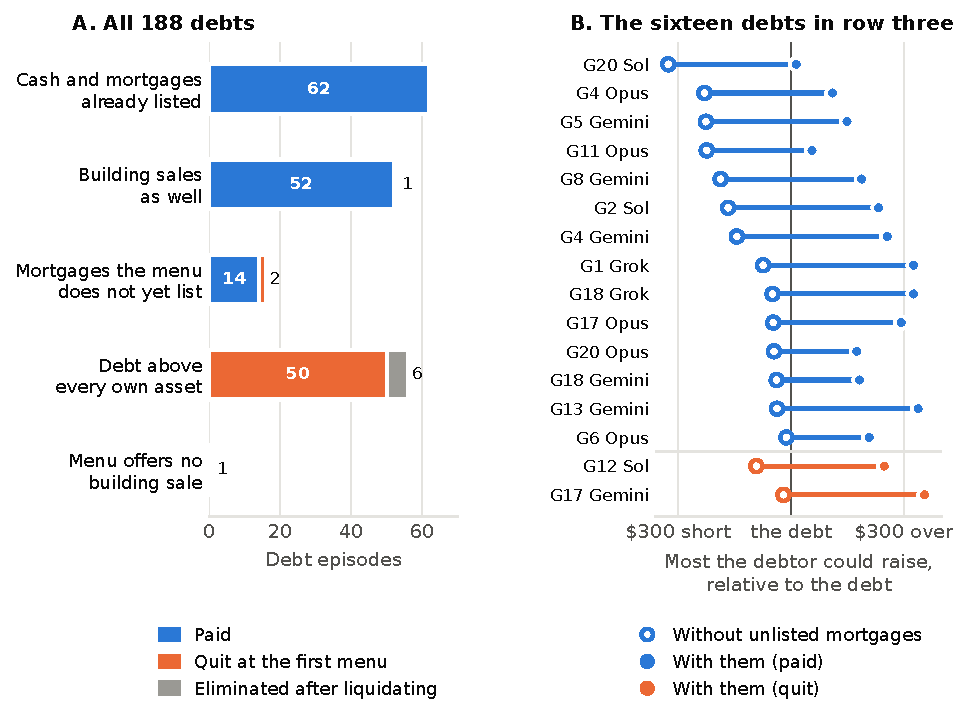
\includegraphics[width=\linewidth]{debt_partition.pdf}
\caption{Debts and what they required. A: every debt episode, by the least the first menu required and by outcome. B: the sixteen debts in the third row. The open circle is the most the debtor could raise from cash, listed mortgages and all building sales. The filled circle adds the mortgages that selling those buildings would release. Every case starts short of the debt and ends beyond it. The two debtors that quit are at the bottom.}
\label{fig:debt}\end{figure}

\subsection{Sixteen debts that needed mortgages the menu did not list}
The third row of Table~\ref{tab:debt} is the hard set. In these sixteen episodes, cash plus every listed mortgage plus the sale of every building still fell short, by a median of \$\fact{d.necessary.median-shortfall-without-unlisted} (Figure~\ref{fig:debt}B). Payment had to use deeds that the first menu did not offer and that no prompt mentions as a resource. An agent that adds up what the menu lists concludes that it cannot pay.

Agents paid fourteen of the sixteen (Table~\ref{tab:sixteen}). Thirteen began by selling buildings, one mortgaged a listed deed first, and all fourteen then mortgaged at least one released deed. The payments took two to ten actions, with a median of \fact{d.necessary.median-actions-paid}. The cases come from twelve games and all five seed blocks, and every system has at least two.

\begin{table}[t]\centering\footnotesize
\TableSixteen
\caption{The sixteen payable debts that required unlisted mortgages. ``Reach without unlisted'' is cash plus listed mortgages plus full building salvage. ``Channel'' is where the text stored at the first decision comes from: the applied private note, or the provider-returned explanation where Opus answered through action-only recovery. The next column is the drafting assistant's reading of what that text does with the unlisted mortgages, with exact spans in Appendix~\ref{app:debts}.}
\label{tab:sixteen}\end{table}

The text stored at the first decision separates the outcomes. In thirteen of the fourteen payments it counts the unlisted mortgages before any building is sold. Gemini's note in G5 is typical:
\TranscriptQuote{g5-d263-note}
The provider-returned text of the same response shows the sum being revised: \InlineQuote{in-g5-d263-revise} The fourteenth payment, Opus in G20, raises the released mortgages as a question without a total. In both failures the text adds up the listed items only. Gemini in G17 held the same two dark-blue deeds it had counted in G5:
\TranscriptQuote{g17-d234-note}
Park Place and Boardwalk would have added \$375 after the sales. Sol in G12 left out \$340 of red mortgages in the same way:
\TranscriptQuote{g12-d190-note}
Both agents declared bankruptcy in that response. Sol counts released mortgages in G2 and in G20.

Nine of the fourteen successful texts are applied private notes, which the same agent reads on later turns. Five are Opus's provider-returned explanations, because recovery responses carry no note. The stated figures can be checked. Of \fact{x.nc.numbers.checked} stated totals, gaps or remainders, \fact{x.nc.numbers.equal} equal the value computed from the records. The exception is Sol's \$430 for yellow mortgages worth \$400, which did not affect the payment. Since the prompt supplies none of these values, each one is a board fact the system recalled.

This result reaches level three with accurate content. The statement comes before the action, its arithmetic is correct in all but one case, and the choice to continue or quit agrees with it in all sixteen. It does not reach level four. No pair of cases differs only in the unlisted collateral, and two failures cannot show that the omission produced the bankruptcy. The text also does not show how the choice was computed.

\subsection{One payment followed from both sides}
\IncidentTitle{g20pay}{A creditor's estimate and a debtor's plan agree on \$1,414}
At G20 turn 107 only Gemini and Sol remain. Sol has \$49, nine orange houses and two brown hotels. Before adding a hotel that raises one rent to \$1,400, Gemini writes down what Sol could raise:
\TranscriptQuote{g20-d325-creditor}
Sol lands there on the next turn. Its first menu lists three mortgageable deeds worth \$325, and its note states a budget before any action:
\TranscriptQuote{g20-d327-plan}
Sol sells its development in two actions and mortgages eight deeds, five of them released by the sales. Its note at the last one reads:
\TranscriptQuote{g20-d336-last}
The events show \$700 from sales and \$665 from mortgages, so $49+700+665-1{,}400=14$. Gemini's total was also right, although its two components were each off by \$25 in opposite directions. Sol was eliminated seven turns later and Gemini won.
\IncidentSource{G20 d325 and d327 to d336, standard responses. All three quotations are private notes and were not delivered to the other player. Sales, mortgages, the rent and the \$14 balance are read from events and the next prompt.}

The case shows an announced total carried through ten applied actions to the dollar. Sol stated one aggregate budget and a rule, to sell everything and then mortgage everything. Once the buildings were gone, the eight mortgages could be made in any order, and each refreshed menu showed what remained. Ten actions are not ten steps of lookahead. What Sol fixed in advance was the total, the decision not to concede, and the reliance on \$340 of collateral that the first menu did not list.

Nineteen payments used a mortgage that was absent from the first menu. Fourteen are the cases above. In the other five the released deeds were one way to pay among several. The third payable bankruptcy, Grok in G12, was not a failed sum. Its note says \InlineQuote{in-g12-d249-note} The text outside its tool call names a two-house sale, and the call that arrived declared bankruptcy.

\section{A rival's options: the completing deed}
\label{sec:rival}

\subsection{What happens to an offer that completes the proposer's group}
The agents answered \fact{o.census.responses.n} offers with \fact{o.census.responses.accept} acceptances, \fact{o.census.responses.counter} counters and \fact{o.census.responses.reject} rejections. Each system accepted between \fact{o.census.by-recipient.Gemini.accept} and \fact{o.census.by-recipient.Sol.accept} offers. They differ in how they disagree: Sol and Opus countered \fact{o.census.by-recipient.Sol.counter} and \fact{o.census.by-recipient.Opus.counter} times, and Gemini and Grok rejected \fact{o.census.by-recipient.Gemini.reject} and \fact{o.census.by-recipient.Grok.reject}.

A deed that would complete the proposer's color group is the clearest case of a move that opens something for a rival, because only a complete group can be built on. Table~\ref{tab:opening} gives every opening offer by form and by who would complete a group. We compare opening offers because later offers are shaped by what both sides have already refused (Appendix~\ref{app:offers}).

\begin{table}[t]\centering\small
\TableOpening
\caption{All \fact{o.census.opening} acceptance-legal opening offers. A swap moves deeds both ways. A cash bid offers only cash for deeds. A sale offer offers only deeds for cash. ``Other'' holds the remaining forms. Completion is evaluated on ownership after the proposed transfer. Empty cells are omitted: a cash bid cannot complete the recipient's group and a sale offer cannot complete the proposer's.}
\label{tab:opening}\end{table}

An opening swap or cash bid that would complete only the proposer's group was accepted \fact{x.po.accept} times in \fact{x.po.n}. Recipients rejected \fact{x.po.reject} and countered \fact{x.po.counter}. The same two forms, when they completed nobody's group, were accepted \fact{x.nei.accept} times in \fact{x.nei.n}.

\subsection{Swaps are refused and cash bids are priced}
The response depends on what the proposer puts on the table. Recipients rejected \fact{o.headline-cells.swap-proposer-only.reject} of \fact{o.headline-cells.swap-proposer-only.n} swaps that completed only the proposer (\fact{x.swpo.rej.pct}\%) and \fact{o.headline-cells.swap-neither.reject} of \fact{o.headline-cells.swap-neither.n} that completed nobody (\fact{x.swn.rej.pct}\%), a gap of \fact{o.sensitivity.swap-gap.point-pp} percentage points. Swaps that completed both sides fall between, at \fact{o.headline-cells.swap-both.reject} of \fact{o.headline-cells.swap-both.n}. For cash bids the two rates are \fact{o.headline-cells.cash-bid-proposer-only.reject} of \fact{o.headline-cells.cash-bid-proposer-only.n} and \fact{o.headline-cells.cash-bid-neither.reject} of \fact{o.headline-cells.cash-bid-neither.n}, a difference of \fact{o.sensitivity.cash-bid-gap.point-pp} points (Figure~\ref{fig:offers}A).

\begin{figure}[t]\centering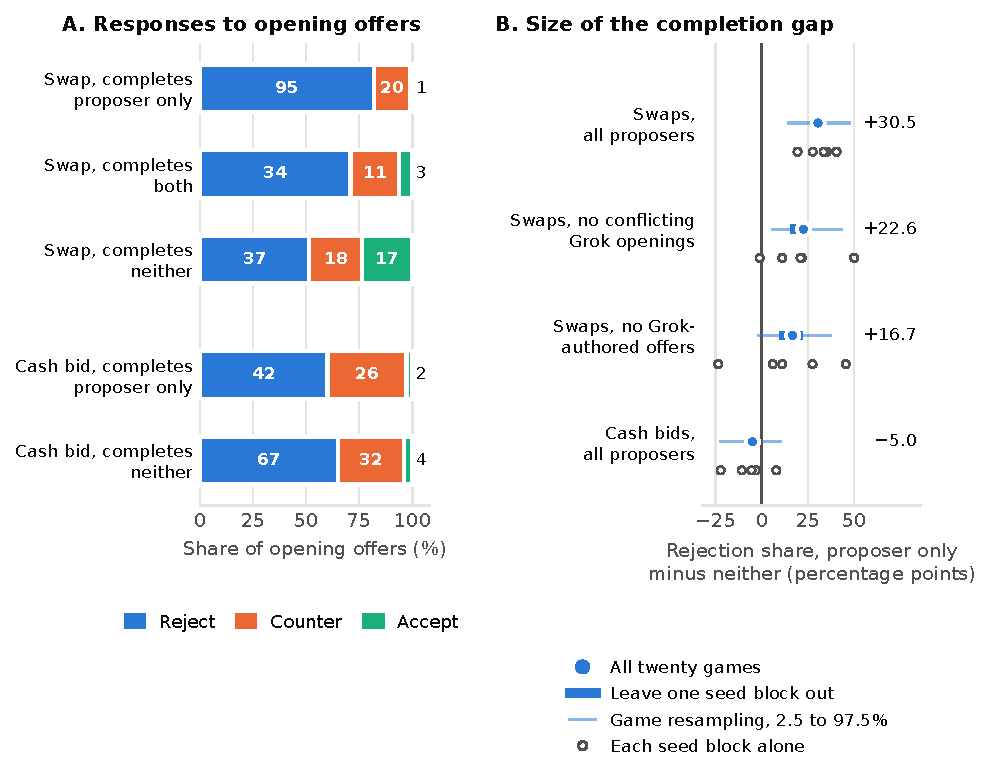
\includegraphics[width=\linewidth]{offer_responses.pdf}
\caption{Opening offers. A: responses by form and completion, as shares with counts printed. B: the rejection share for offers completing only the proposer minus the share for offers completing nobody. The dot uses all twenty games. The thick bar is the range when one seed block is left out. The thin line spans the middle 95\% of 20,000 resamples of the twenty games. Open circles are the five seed blocks taken alone. These describe how one cohort's contrast depends on its games. They are not intervals for new games.}
\label{fig:offers}\end{figure}

The swap gap holds in direction for every recipient, every proposer and every seed block (Table~\ref{tab:strata}). Its size depends on who wrote the comparison offers. Grok wrote \fact{o.composition.swap-neither-by-grok} of the \fact{o.headline-cells.swap-neither.n} swaps that completed nobody and \fact{o.composition.swap-neither-accepted-by-grok} of the \fact{o.composition.swap-neither-accepted} that were accepted, and \fact{o.composition.swap-neither-accepted-conflict-openings} of those acceptances answered openings whose text named a different action. Without the conflicting openings the gap is \fact{o.sensitivity.swap-gap-without-conflict-openings.point-pp} points. Without any Grok-authored swap it is \fact{o.sensitivity.swap-gap-without-grok-authors.point-pp} points (\fact{o.composition.without-grok-authors.swap-proposer-only.0} of \fact{o.composition.without-grok-authors.swap-proposer-only.1} against \fact{o.composition.without-grok-authors.swap-neither.0} of \fact{o.composition.without-grok-authors.swap-neither.1}). Weighting the within-proposer gaps by three choices of proposer mix gives \fact{o.composition.standardized-swap-gap-pp.weights-proposer-only-cell} to \fact{o.composition.standardized-swap-gap-pp.weights-neither-cell} points. Removing offers shows how the count depends on them, not what the other agents would have done in games without them. Table~\ref{tab:sens} gives the ranges under each version. Leaving out any one seed block keeps the gap positive in every version. In the version without Grok's offers both resampling ranges reach below zero, and in both reduced versions one seed block taken alone is negative.

\begin{table}[t]\centering\small
\TableStrata
\caption{Rejected over received, opening offers, by proposer and by recipient. Within every recipient the swap gap is positive (\fact{x.rec.Opus.swgap} to \fact{x.rec.Sol.swgap} points) and the cash-bid gap is between \fact{x.rec.Opus.cbgap} and \fact{x.rec.Sol.cbgap} points. Opus wrote \fact{o.composition.cash-bids-in-headline-cells-by-opus} of the \fact{o.composition.cash-bids-in-headline-cells} cash bids.}
\label{tab:strata}\end{table}

\begin{table}[t]\centering\footnotesize
\TableSensitivity
\caption{How the selected contrasts depend on the games included. Values are percentage points. ``Seed-block resampling'' is the 2.5th to 97.5th percentile over all 3,125 ordered resamples of five blocks. ``Game resampling'' is the same percentiles over 20,000 resamples of twenty games. The contrasts were chosen after inspecting these games, and the games share seeds and one roster, so the ranges describe this cohort and are not confidence intervals.}
\label{tab:sens}\end{table}

For cash bids the pooled difference is negative, the difference within each recipient lies between \fact{x.rec.Opus.cbgap} and \fact{x.rec.Sol.cbgap} points, and both resampling ranges include zero. These records show no completion gap for cash bids. They do not show that one is absent.

What differs is the kind of reply. Recipients countered \fact{o.headline-cells.cash-bid-proposer-only.counter} of \fact{o.headline-cells.cash-bid-proposer-only.n} completing cash bids (\fact{x.cbpo.ctr.pct}\%) and \fact{o.headline-cells.swap-proposer-only.counter} of \fact{o.headline-cells.swap-proposer-only.n} completing swaps (\fact{x.swpo.ctr.pct}\%), a difference with the same sign in all five seed blocks. In \fact{o.counters.opening-cash-bid-proposer-only.same-bundle-more-cash} of the \fact{o.counters.opening-cash-bid-proposer-only.counters} cash-bid counters the recipient kept the deeds as proposed and asked for more money.

\subsection{What the refusals say, and how the systems differ}
The stated reasons do not separate the two forms. A pattern match finds completion or blocking language in \fact{o.keyword-screen.rejections.swap-proposer-only.completion-terms} of the \fact{o.keyword-screen.rejections.swap-proposer-only.n} rejections of completing swaps and in all \fact{o.keyword-screen.rejections.cash-bid-proposer-only.n} rejections of completing cash bids, and building language in \fact{o.keyword-screen.rejections.swap-proposer-only.building-terms} and \fact{o.keyword-screen.rejections.cash-bid-proposer-only.building-terms}.

\begin{table}[t]\centering\small
\TableStyles
\caption{Responses to the \fact{x.po.n} opening swaps and cash bids that would complete only the proposer's group, by recipient. The right-hand columns are regular-expression counts over the public message and applied note of each rejection: building terms (house, hotel, build, develop), reciprocity terms (``in return'', ``for me as well'' and similar) and commitment terms (``never'', ``not for sale'', ``do not counter''). Opus answered \fact{x.opus.recovery.trade.responses} of its \fact{o.census.by-recipient.Opus.n} trade responses through action-only recovery, without a note.}
\label{tab:styles}\end{table}

The systems refuse in recognizably different ways (Table~\ref{tab:styles}). Gemini rejected \fact{x.style.Gemini.rej.pct}\% of these openings and often stated a rule, as in G4: \InlineQuote{in-g4-d72-rule} Grok rejected \fact{x.style.Grok.rej.pct}\% and paired dollar estimates of the rival's building cash with a commitment not to bargain, as in G1: \InlineQuote{in-g1-d122-commit} Sol rejected \fact{x.style.Sol.rej.pct}\% and countered the rest. Opus countered \fact{o.refusal-wording.responses-by-recipient-proposer-only-openings.Opus.counter} of \fact{o.refusal-wording.responses-by-recipient-proposer-only-openings.Opus.n}.

An earlier coding of stated reasons in this project covers a different population. Two model-assisted readings agreed that \fact{o.semantic-codes.agreed-rival-consequence} of \fact{o.semantic-codes.coded-rows} rejections named a consequence for the rival. All \fact{o.semantic-codes.coded-rows} are rejections of offers that would complete the recipient's own group, so none falls in the cells compared above. They show that agents state rival concern even when refusing their own monopoly, and they cannot explain why swaps and cash bids are treated differently. Incident 2 is one of those refusals.

\IncidentTitle{g15}{Refusing one's own monopoly to deny a rival's}
At G15 turn 63 Sol holds \$730 and two greens. Grok holds \$333, the third green and Ventnor, the yellow Sol lacks. One turn earlier Opus had told the table, \InlineQuote{in-g15-d166-appeal}. Sol offers both greens for Ventnor and \$100, which would complete a group for each side. Grok refuses, and its note compares what each could then build:
\TranscriptQuote{g15-d169-note}
The cash figures are right. A first row of green houses does cost \$600, although a single \$200 house would have been legal. Sol drops the cash request and adds Kentucky, is refused again, and then restates the comparison in Grok's terms:
\TranscriptQuote{g15-d174-sweetener}
\TranscriptQuote{g15-d175-refusal}
All three offers fail, and Gemini refuses a different Sol offer on the same turn. Eighteen turns later Grok goes bankrupt to Gemini, which inherits its deeds and wins. Sol never completes yellow or green. Whether accepting would have served Grok better is not known.
\IncidentSource{G15 d166 to d176, standard responses. The Opus appeal is in Grok's prompt at d169. Each public message appears in the counterparty's next prompt.}

\subsection{Does refusal follow the size of the rival's opportunity?}
Grok's note in G15 reasons about amounts: how much the rival would hold and how many houses that buys. If refusals in general followed that reasoning, they would be more common when the proposer would keep more building cash. They are not. Among completing swaps, recipients rejected \fact{o.rival-capacity.swap-proposer-only.1-2.reject} of \fact{o.rival-capacity.swap-proposer-only.1-2.n} when the proposer could afford one or two houses after the trade, \fact{o.rival-capacity.swap-proposer-only.3-5.reject} of \fact{o.rival-capacity.swap-proposer-only.3-5.n} for three to five, and \fact{o.rival-capacity.swap-proposer-only.6+.reject} of \fact{o.rival-capacity.swap-proposer-only.6+.n} for six or more. When the proposer could afford none, they rejected \fact{o.rival-capacity.swap-proposer-only.0.reject} of \fact{o.rival-capacity.swap-proposer-only.0.n}, too few to read. Completing cash bids show no order either (Appendix~\ref{app:offers}). The measure ignores what the proposer could still mortgage, so it is coarse.

A crude check speaks against the simplest alternative, that completing swaps are refused because they pay badly. At board list prices the completing swaps offered the recipient more, a median of \$\fact{o.list-value.swap-proposer-only.median-net-list-value-to-recipient} against \$\fact{o.list-value.swap-neither.median-net-list-value-to-recipient}. Among swaps that favored the recipient at list price, \fact{o.list-value.swap-proposer-only.favourable-to-recipient.0} of \fact{o.list-value.swap-proposer-only.favourable-to-recipient.1} completing ones were rejected and \fact{o.list-value.swap-neither.favourable-to-recipient.0} of \fact{o.list-value.swap-neither.favourable-to-recipient.1} of the others. List price leaves out mortgages, group value and the value of blocking, so this narrows the alternative without removing it. The stated amounts are also not always right.

\IncidentTitle{g2}{A price set on the buyer's building budget, with the wrong house count}
At G2 turn 44 Grok, which owns no yellow, bids \$200 for Sol's Marvin Gardens, and Sol asks \$450. On turn 45 Opus, which owns the other two yellows and has \$845, bids \$325 for the same deed. Sol asks \$650 and records why:
\TranscriptQuote{g2-d124-note}
Both subtractions are right. The house count is wrong. Yellow houses cost \$150, so \$520 buys three. Opus raises to \$450 and says \InlineQuote{in-g2-d127-final} Its note keeps a higher limit: \InlineQuote{in-g2-d127-ceiling} Sol declines:
\TranscriptQuote{g2-d128-keep}
Twenty-four turns later the positions reverse. Opus has \$17 and sells its two yellows to Sol for two railroads and \$100. Sol builds two houses, later sells them, collects \$44 of yellow rent in total, and both players go bankrupt to Gemini.
\IncidentSource{G2 d118 to d128 and d196 to d198. Sol and Opus respond under the standard prompt on turn 45, so both notes are applied private notes. Opus's sale on turn 69 is an action-only recovery response. Opus's ``final'' message is in Sol's prompt at d128.}

The rival side therefore reaches level three and stops there. The agents state a consequence for the rival before they refuse, and the refusals agree with the statements. The content is accurate in some cases and wrong in others. The response follows the event of completion and the form of the offer. It does not follow the measured size of what the rival could do next, which level four would require.

\section{Third parties, and what the agents use talk for}
\label{sec:talk}

A trade between two players can change what a third player gets. Because a bankrupt player's deeds pass to its creditor, keeping a weak player solvent can keep a monopoly away from someone else, and letting it fail can deliver one. Of the \fact{d.eliminations.nonterminal} eliminations that left at least two players in the game, \fact{d.eliminations.nonterminal-to-eventual-winner} sent the estate to the eventual winner. The agents bargain over this prospect in so many words.

\IncidentTitle{g13}{A deed sold as insurance against a third player's inheritance}
At G13 turn 107 Grok has \$35, owns the yellow group and stands nine squares before Sol's Short Line, where it would owe \$200. It offers its mortgaged Pennsylvania Avenue to Opus for \$200:
\TranscriptQuote{g13-d250-insurance}
Opus counters at \$130. Grok holds at \$200 and says publicly that \$130 leaves it \$35 short. Its private note records that \$130 would be enough if it also mortgaged Ventnor. The provider-returned text of the same response states the omission:
\TranscriptQuote{g13-d252-omission}
Opus accepts at \$200 and pays \$16 of transfer interest. Its returned explanation takes up the estate argument:
\TranscriptQuote{g13-d253-buyer}
The inheritance the seller describes follows from the rules. Its public odds of 5 in 36 overstate a direct roll of nine, which is 4 in 36. Its own note uses the correct figure: \InlineQuote{in-g13-d252-floor}. With \$130 from the sale, \$35 in hand and the unmentioned \$130 mortgage, it could have paid the rent. Opus's text repeats the estate concern and does not address the financing claim. The records do not show that the omission produced the extra \$70. Grok missed Short Line on its next roll. Opus completed green at auction seven turns later. At turn 150 Grok did go bankrupt on Short Line, and the yellows passed to Sol, the outcome the sale had been pitched to prevent. Opus won.
\IncidentSource{G13 d250 to d253, with later events. Opus responds through action-only recovery, so its text is a provider-returned explanation. Grok's omission statement is also provider-returned text. Both of Grok's public messages appear in Opus's next prompts.}

The estate argument concerns a rival's options two steps removed: what Sol would gain if Grok failed. Both parties state it, the purchase agrees with it and its premise is correct. Like the refusals in Section~\ref{sec:rival}, it is level three.

Four further incidents, documented the same way in Appendix~\ref{app:cases}, show what else the agents do with public messages under a prompt that permits deception.

\emph{A bluff with a recorded ceiling.} In G7 Grok bids \$600 for a deed and calls the offer final, while its note says to accept \$625. The seller accepts \$600. Later the same seller, short of cash after building, sells a completing deed to Gemini for twice Gemini's bid. Gemini's note times the bid to the seller's need for building cash, the seller's note sets a price that funds its own houses and leaves Gemini little, and both build within eight turns.

\emph{A false premise corrected.} In G19 a Grok proposal reaches Sol with a claim that a pink deed is orange. Sol replies that the deed is pink and accepts the trade on its terms. Grok's own note in that response says to abort the trade, and the text outside its tool call names a different action.

\emph{A call to withhold cash.} In G20 Gemini asks the table not to buy a cash-poor rival's spare deeds, because the money would become houses on its new monopoly. Gemini then refuses such a sale itself. Opus later makes the opposite offer and describes it as money for more houses. No sale settles.

\emph{An assurance withdrawn.} In G18, with two players left, Opus tells Sol that its \$250 offer for a deed still stands. Text returned with that response says Opus had not raised the offer because extra cash would help the opponent last longer. One turn and one \$750 rent later, Sol tries to take the offer and Opus withdraws it, with the same stated reason. No Opus text in this stretch mentions inheriting anything. The stated motive is to deny the last opponent the cash to survive.

Each of these is one trajectory, chosen because it is clear. They are not a sample and do not measure how often agents bluff, omit, correct or coordinate.

\section{Discussion}
\label{sec:discussion}

\paragraph{What the two results share, and where they differ.}
In both settings the agents wrote down a consequence that the terms in front of them did not show, and then acted in line with it. The debt result can be checked in a way the bargaining result cannot. Whether a debt needs unlisted mortgages follows from four sums and the rules, so the hard cases are defined without reference to what any agent did or said. In those cases the stated arithmetic was right in all but one instance, and the action matched the statement every time. The systems that left out released collateral once counted it in other games, so the two failures are lapses and do not mark a limit of any system.

In bargaining, the consequence is a judgment about value: how much a rival's monopoly will cost the holder later. The agents stated that judgment and refused accordingly, but their refusals tracked the event of completion and the form of the offer. They did not track the amount of building the rival could afford, and some stated amounts were wrong. Two systems declined almost every such opening under an announced rule or commitment. A rule of that kind may be a sound response to an opportunity that is hard to price. It is also what an agent would do if the word ``monopoly'' alone drove the refusal. The records cannot separate the two.

\paragraph{Why form might matter.}
A counter to a cash bid changes one number, while a swap requires valuing two bundles and the rival's gain together. The swaps on offer may also have been worse in ways list prices miss, and proposer mix differs across the cells. A test would hold the recipient's side of the offer fixed and vary only whether the proposer completes a group, and separately vary how much the proposer could then build.

\paragraph{The systems are configured systems.}
The response conditions are part of what was measured. Opus played without private notes after the first games, and Grok's offers include many that its own text disowned and that other agents accepted. With several agents in one game, a change to one participant's interface changes the offers every other participant sees.

\section{Related work}
\label{sec:related}

\paragraph{Negotiation with language models.}
Early neural negotiation agents were trained on dialogues with hidden rewards~\cite{lewis2017deal}. NegotiationArena evaluates LLM bargaining in defined scenarios and reports that tactics such as feigned desperation change payoffs~\cite{bianchi2024negotiationarena}. Cosentino et al.\ find that agents can model a counterpart's preferences accurately and still fail to turn that into better outcomes~\cite{cosentino2026counterparty}. Our levels of evidence follow that line. Those studies have an explicit payoff for each agreement and controlled variation, which ours lacks. Ours has persistent consequences: a trade changes who can build, who goes bankrupt and who inherits.

\paragraph{Externalities and trade restrictions.}
Economic theory treats sales in which the identity of the buyer changes the position of others. Jehiel and Moldovanu show that such externalities can delay agreement~\cite{jehiel1995delay}, and Jehiel, Moldovanu and Stacchetti study sales that affect the later interaction among potential buyers~\cite{jehiel1996nuclear}. A completing deed is an object of this kind, and the G13 sale is priced on a harm to a third party. We use the idea descriptively and test no equilibrium prediction. Refusing trades that help a rival is also not new to LLM agents. Guhe and Lascarides study persuasion and trade embargoes among symbolic agents in Settlers of Catan and measure their effect on winning in controlled simulations~\cite{guhe2014persuasion}. Our records show free-form versions of such refusals without the comparison that would say whether they help.

\paragraph{Monopoly and economic agent benchmarks.}
AgentMonopoly varies model family, size and persona in four-player Monopoly and reports trade frequency and acceptance~\cite{wu2026agentmonopoly}. FinBoardBench covers financial management across board games and finds that models buy assets while short of cash~\cite{hu2026finboardbench}. Cattle Trade pits LLMs against scripted agents and relates resource discipline to rank~\cite{muller2026cattletrade}. Li et al.\ check inter-agent messages in long commerce simulations against simulator state, with a reference set and several judge models~\cite{li2026arena}. Playing Monopoly, countering offers and managing cash are therefore not our contribution. We add a complete census of offers and debts paired with the text recorded before each action, and the split of debts by what the first menu could raise.

\paragraph{Planning and stated reasons.}
PlanBench evaluates plan generation and reasoning about change in planning domains and reports that LLMs fall well short on plan generation~\cite{valmeekam2023planbench}. Debt payment here is a different task. Execution has feedback because the menu refreshes after each action. The decision to continue has none, and the sixteen cases place the test there. Explanations produced by language models need not reflect the process that produced the answer~\cite{turpin2023unfaithful,lanham2023faithfulness}, so we compare each note with the state and the action and do not treat it as evidence of how the action was chosen.

\section{Limitations}
\label{sec:limits}

The cohort is twenty games from five seeds, one roster and one cyclic seat order. It cannot separate a system from its seat, its opponents or its luck, and it supports no ranking. Wins were \fact{p.wins-by-system.Sol}, \fact{p.wins-by-system.Gemini}, \fact{p.wins-by-system.Opus} and \fact{p.wins-by-system.Grok} for Sol, Gemini, Opus and Grok, and \fact{p.wins-by-seat.1}, \fact{p.wins-by-seat.2}, \fact{p.wins-by-seat.3} and \fact{p.wins-by-seat.4} by seat.

Every contrast was selected after the games were inspected, and no new games were run to confirm any of them. The sixteen hard debts include only two failures. The offer comparisons differ in terms, counterparties and timing as well as in completion and form. No reference policy, value estimate or human annotation is available, so nothing here says whether a refusal, a price or a liquidation was good play. Whether a rule that takes any listed financing action would pay the same debts is untested. Such a rule would never face the decision to quit, where both failures occurred.

The readings of text come from language-model assistants, some from the same model families as two participants, and exact spans are printed so that a reader can check them. The three payment sequences behind the payable bankruptcies and the replay comparisons are inherited from earlier work in this project. The prompt invites public deception, so the incidents show permitted conduct. The response conditions for Opus and Grok shaped what every player faced.

\section{Conclusion}
\label{sec:conclusion}

Across twenty complete games, LLM agents stated what a move would make possible before they made it, and their actions agreed with those statements. For their own debts the statements were accurate. Agents almost always quit when no payment existed and continued when one did. They paid fourteen of the sixteen debts that could be met only with mortgages absent from the menu, and in thirteen of those they had counted that collateral before acting. For rivals the statements were as frequent and less exact. Agents almost never accepted an opening that completed only the proposer's group, they refused swaps and put prices on cash bids, and their refusals followed the event of completion without following how much the rival could then build. Whether these choices were good ones, and whether they hold in a new cohort, are questions for controlled tests.

\begingroup\small
\bibliographystyle{plainnat}\bibliography{references}
\endgroup
\clearpage\appendix
\section{Casebook: four further incidents}
\label{app:cases}

Incidents 1 to 4 are in the main text. Incidents 5 to 8 follow, with the same elements: the economic situation, exact quotations with their channel, what the counterparty received, a reading at the levels of Section~\ref{sec:setting}, and what happened next. Table~\ref{tab:incidents} indexes all eight.

\begin{table}[ht]\centering\small
\begin{tabularx}{\linewidth}{@{}rlL{.30\linewidth}Y@{}}\toprule
 & Game & What was stated & What the records support\\\midrule
1 & G20 & Debtor's private budget of \$1,414 against a \$1,400 rent; creditor's private estimate of the same total & Accurate and carried out in ten actions; \$14 left\\
2 & G15 & Private comparison of post-trade building cash; public refusal & Cash figures accurate; three offers refused; outcome of the alternative unknown\\
3 & G2 & Private pricing note on the buyer's remaining cash; public ``final'' offer below a private ceiling & Subtraction right, house count wrong; ask \$200 above the ask to a non-completing buyer\\
4 & G13 & Public estate-insurance pitch; returned text describing an omission & Premise correct, odds overstated, financing omitted; effect of the omission not identified\\
5 & G7 & Public ``final'' bid with a private ceiling; private notes tying a payment to both sides' houses & Bluff untested; stated cash figures accurate; both sides build\\
6 & G19 & Public claim that a pink deed is orange; recipient's public correction & Recipient corrects the claim and accepts on the terms; sender's channels disagree\\
7 & G20 & Public appeal not to fund a rival's houses & Author follows through; another player makes the opposite offer; no effect measured\\
8 & G18 & Public assurance that an offer stands; public withdrawal; returned reasons & Stated reason is survival cash for the last opponent; no inheritance statement\\
\bottomrule\end{tabularx}
\caption{The eight incidents. They were chosen for clarity and variety, and they are not a sample of conduct.}
\label{tab:incidents}\end{table}

\IncidentTitle{g7}{A public final offer under a private ceiling, then a payment priced on both sides' houses}
At G7 turn 25 Sol has just bought North Carolina for \$300 and asks Grok \$650 for it. Grok bids \$575, Sol asks \$625, and Grok replies:
\TranscriptQuote{g7-d42-final}
Its note leaves room above that figure:
\TranscriptQuote{g7-d42-ceiling}
Sol accepts \$600. The public limit sits \$25 below the private one. Because the seller accepted, the records do not show what Grok would have done at \$625.

At turn 67 Sol pays Opus \$800 and States Avenue for Park Place, builds three dark-blue houses and is left with \$84. Gemini holds two oranges. On the next turn it bids \$350 for Sol's New York Avenue, and its note ties the bid to Sol's position:
\TranscriptQuote{g7-d141-bid}
Sol asks \$700 and writes:
\TranscriptQuote{g7-d142-ask}
Both of Sol's figures are right. With \$784 it can add the three houses that bring each dark blue to three and keep \$184, and Gemini would hold \$45. Gemini offers \$520, Sol holds at \$700, and Gemini pays it. Gemini mortgages five deeds and builds four orange houses that turn. Sol adds three dark-blue houses within eight turns. Gemini collects \$270 of orange rent before Sol eliminates it at turn 125. Sol wins.

Both notes state what the payment would let each side build, with correct amounts, and both sides then build. This is level three for a statement that covers the writer's own options and the rival's at once. The price cannot be judged without a value reference.
\IncidentSource{G7 d39 to d43 and d137 to d149, standard responses. Grok's ``final'' message is in Sol's prompt at d43. The notes are private.}

\IncidentTitle{g19}{A false premise corrected by the recipient}
At G19 turn 67 a proposal from Grok reaches Sol: Virginia and \$150 for States. Both deeds are pink. The public message sent with it says:
\TranscriptQuote{g19-d135-public}
Sol owns two oranges, and the trade completes no group for either side. Sol answers:
\TranscriptQuote{g19-d136-public}
The trade executes. Sol's note judges the terms and adds \InlineQuote{in-g19-d136-note}

The proposal is not a clean statement of intent. The applied note in the same Grok response reads:
\TranscriptQuote{g19-d135-note}
The text outside the tool call names \texttt{end\_turn}. The call that arrived was a trade proposal, and the engine sent it.

Sol checks a stated premise against the board, corrects it in public and evaluates the terms on their own. That is an accurate assessment of another player's claim. The false claim cannot be read as a planned deception, because the sender's channels disagree with one another.
\IncidentSource{G19 d135 and d136, standard responses. The false message is in Sol's prompt at d136, and Sol's reply is in Grok's prompt at d137.}

\IncidentTitle{g20appeal}{A public call not to fund a rival's houses}
At G20 turn 22 Opus sells Illinois to Grok for \$500. Grok now owns the red group and has \$222. On turn 25 Gemini ends its turn with:
\TranscriptQuote{g20-d96-appeal}
Grok's note at its next decision registers the message:
\TranscriptQuote{g20-d97-note}
On turn 27 Grok builds one house on each red, mortgages New York and offers Vermont to Gemini for \$150, saying the money is not a house fund. Gemini refuses:
\TranscriptQuote{g20-d101-refusal}
Grok mortgages Vermont for \$50. Ten turns later Opus offers Grok \$140 for mortgaged New York and says, \InlineQuote{in-g20-d129-houses}. Neither that offer nor a later one settles. Grok is the first player eliminated, and Gemini wins.

The appeal is a public statement about a rival's options, and its author acts on it when tested. Another player pursues the opposite bargain. The records show no agreement among the others and no measure of the appeal's effect.
\IncidentSource{G20 d83, d96 to d102 and d129. The appeal is in Grok's prompt at d97. Opus's d129 message is an action-only recovery response.}

\IncidentTitle{g18}{An assurance withdrawn to deny the last opponent survival cash}
At G18 turn 181 only Opus and Sol remain. Opus holds two mortgaged greens. Sol holds the third, Pacific, also mortgaged. Opus bids \$200, Sol asks \$600, and Opus offers \$250 as final. At turn 187, after Sol pays it \$750 in rent, Opus ends its turn with:
\TranscriptQuote{g18-d431-assurance}
Text returned with the same response gives a reason for going no higher:
\TranscriptQuote{g18-d431-content}
On turn 188 Sol pays another \$750, sells buildings, mortgages deeds and is left with \$49. It offers Pacific in two packages at \$450 and \$350, and then:
\TranscriptQuote{g18-d441-invocation}
\TranscriptQuote{g18-d442-withdrawal}
\TranscriptQuote{g18-d442-explanation}
Opus then redeems its two greens on turns 190 and 192 and bids \$150 and \$225 for Pacific on turn 194. Sol asks \$450, \$350 and \$300. Nothing settles. Sol is eliminated at turn 197, and Opus wins.

The reason Opus's returned text gives is the same before and after the withdrawal: cash would help the last opponent survive. With two players left, Sol's bankruptcy ends the game, so the deeds Opus receives then have no later use. The case concerns survival cash and does not show bargaining for an inheritance. Opus's later bids came after it had redeemed its greens, which changed what completing the group would cost, and they stayed below the withdrawn price. No record shows that the assurance was insincere when made, or that Sol lost anything by relying on it.
\IncidentSource{G18 d419 to d461. Opus responds through action-only recovery, so its reasons are assistant content and provider-returned text, neither delivered to Sol. The assurance is in Sol's prompt at d441 and in Opus's own prompt at d442.}

\section{Offer tables}
\label{app:offers}

Table~\ref{tab:fulloffers} gives every acceptance-legal offer by stage, form and completion. Two of the \fact{o.census.responses.n} offers could not legally be accepted and are omitted. Table~\ref{tab:blocks} gives the compared cells for each seed block.

\begin{table}[ht]\centering\small
\TableFullOffers
\caption{All \fact{o.census.acceptance-legal} acceptance-legal offers. Cells show offers (accepted/countered/rejected). Later offers are counters within a thread.}
\label{tab:fulloffers}\end{table}

\begin{table}[ht]\centering\small
\TableBlocks
\caption{The compared opening cells and the unlisted-collateral debts, by seed block. Each block is four games with one seed and four seat rotations.}
\label{tab:blocks}\end{table}

\paragraph{Later offers.}
Among later offers the same four cells show smaller differences: \fact{o.later-cells.swap-proposer-only.reject} of \fact{o.later-cells.swap-proposer-only.n} completing swaps and \fact{o.later-cells.swap-neither.reject} of \fact{o.later-cells.swap-neither.n} other swaps were rejected, and \fact{o.later-cells.cash-bid-proposer-only.reject} of \fact{o.later-cells.cash-bid-proposer-only.n} completing cash bids against \fact{o.later-cells.cash-bid-neither.reject} of \fact{o.later-cells.cash-bid-neither.n}. A later offer exists only because both parties kept talking, so these are not comparable with openings.

\paragraph{Counters.}
Across all stages, \fact{o.counters.all-author-only.same-bundle-more-cash} of \fact{o.counters.all-author-only.counters} counters to offers completing only the proposer kept the deeds and jail cards as proposed and improved the counterer's cash. The figure for deed requests completing nobody is \fact{o.counters.all-neither-deed-requests.same-bundle-more-cash} of \fact{o.counters.all-neither-deed-requests.counters}. Asking for more cash is the usual counter in both groups. Agreement stayed rare after a completing opening: \fact{o.thread-outcomes.cash-bid-proposer-only.settled} of the \fact{o.thread-outcomes.cash-bid-proposer-only.threads} threads opened by a completing cash bid and \fact{o.thread-outcomes.swap-proposer-only.settled} of the \fact{o.thread-outcomes.swap-proposer-only.threads} opened by a completing swap ended in a trade.

\paragraph{The proposer's building capacity.}
Table~\ref{tab:capacity} splits the completing openings by how many houses the proposer could buy on the completed group with its cash after the trade and any transfer interest. Mortgages the proposer could still raise are ignored. Where a trade completes two groups we take the cheaper one.

\begin{table}[ht]\centering\small
\TableCapacity
\caption{Responses to opening offers that would complete only the proposer's group, by the proposer's house capacity after the trade.}
\label{tab:capacity}\end{table}

\paragraph{Pattern matches on rejection text.}
Table~\ref{tab:keywords} counts rejections whose public message or applied note matches a completion or blocking pattern (monopol, complet, set, finish, third, block) or a building pattern (house, hotel, build, develop). These are regular-expression counts and not semantic codes. The \fact{o.keyword-screen.counters.cash-bid-proposer-only.n} counters to completing cash bids match the completion pattern in \fact{o.keyword-screen.counters.cash-bid-proposer-only.completion-terms} cases.

\begin{table}[ht]\centering\small
\TableKeywords
\caption{Pattern matches in the text of rejected opening offers.}
\label{tab:keywords}\end{table}

\paragraph{Composition of accepted openings.}
At board list prices, the \fact{o.composition.accepted-openings-net-list-value-to-recipient.grok-authored.1} accepted openings that Grok wrote gave recipients a net \$\fact{o.composition.accepted-openings-net-list-value-to-recipient.grok-authored.0}, and the \fact{o.composition.accepted-openings-net-list-value-to-recipient.other-authors.1} written by the other systems gave a net \$\fact{o.composition.accepted-openings-net-list-value-to-recipient.other-authors.0}. List price ignores mortgages, group value and blocking value, so this describes the terms and does not value them.

\paragraph{Holder cash.}
Across all stages, holders with under \$100 rejected \fact{o.holder-cash.all-author-only.under-100.reject} of \fact{o.holder-cash.all-author-only.under-100.n} offers completing only the proposer and countered \fact{o.holder-cash.all-author-only.under-100.counter}. Holders with \$300 or more rejected \fact{o.holder-cash.all-author-only.300-plus.reject} of \fact{o.holder-cash.all-author-only.300-plus.n}. The low-cash group is not comparable with the high-cash group: \fact{o.holder-cash.under-100-later-offers} of its \fact{o.holder-cash.all-author-only.under-100.n} offers are later offers and \fact{o.holder-cash.under-100-to-opus} went to Opus. Gemini rejected \fact{o.holder-cash.by-recipient.Gemini.under-100.reject} of \fact{o.holder-cash.by-recipient.Gemini.under-100.n} such offers even when under \$100. We report the association and draw no conclusion about cash pressure from it.

\paragraph{The earlier reason codes.}
The \fact{o.semantic-codes.coded-rows} coded rejections are every rejected offer that would complete the recipient's group: \fact{o.semantic-codes.coded-by-cell.recipient-only} completing the recipient only and \fact{o.semantic-codes.coded-by-cell.both} completing both. The two readings agree on a rival consequence in \fact{o.semantic-codes.agreed-by-cell.recipient-only} and \fact{o.semantic-codes.agreed-by-cell.both} of them. Gemini and Grok account for \fact{o.semantic-codes.agreed-by-recipient.Gemini} and \fact{o.semantic-codes.agreed-by-recipient.Grok} of the \fact{o.semantic-codes.agreed-rival-consequence} agreed cases, and G1 and G15 for \fact{o.semantic-codes.agreed-in-g1-g15}. The codes are model-assisted readings from an earlier stage of this project. We joined them to the offer ledger and did not recode them.

\section{Debt tables}
\label{app:debts}

\TableSixteenQuotes

\paragraph{Other readers.}
Three other assistants read the same sixteen texts independently in an earlier assessment of this project. All three singled out the same tentative case, G20 d291, and one noted that Sol's G20 text states an aggregate budget without listing the mortgages. These are model-assisted readings and not human annotation.

\paragraph{The nineteen uses.}
Nineteen payments include a mortgage on a deed that was absent from the first menu, \fact{d.unlisted-use.mortgages} such mortgages in all. Fourteen are the paid cases in Table~\ref{tab:sixteen}. In the other five the debt could have been met from cash, listed mortgages and building sales: four Gemini payments in G3 (d228, d356, d461, d482) and one Sol payment in G18 (d428).

\paragraph{The three payable bankruptcies.}
For G12 d190 (Sol), G17 d234 (Gemini) and G12 d249 (Grok), an earlier audit of this project applied a legal sequence of sales and mortgages on the engine from the stored state and reached payment. For the first two the sequence sells every building and mortgages the released deeds. The stored sequence for the third sells its seven pink houses in even order, and the first five sales already cover the debt. We read the stored sequences and did not execute them. The first-menu sums computed here agree with them: each debt lies within the full bound.

\paragraph{The menu-restricted elimination.}
At G7 d338 Opus owed \$750 with \$290 in cash, two mortgageable deeds worth \$150, and a pink group holding two four-house lots and a hotel. The bank had no houses, so the hotel could not be broken down, and the even-selling rule left no other sale. The menu listed no building sale. Opus mortgaged both listed deeds, reached \$440 and was eliminated. This reflects the implemented menu. An earlier reading of the validator found that it would accept a bundled sale of the whole group if one were offered.

\paragraph{Debts above every asset.}
Of the \fact{d.above-bound.episodes}, \fact{d.above-bound.declared-at-first-menu} were declared at the first menu. In the other \fact{x.debt.above.continued} the agent mortgaged or sold first, five times Grok and once Gemini, and was eliminated when nothing remained or declared later.

\section{Reproducibility}
\label{app:repro}

\paragraph{Where everything is.}
The repository is \url{https://github.com/KushagraBharti/MonopolyBench}. The twenty runs are in \path{saved_games/railway-research-12-games-2026-10-25/} (G1 to G12) and \path{saved_games/railway-research-8-games-2026-10-26/} (G13 to G20). Each \path{game-NN-*/run/} directory holds \path{events.jsonl}, \path{decisions.jsonl}, \path{actions.jsonl}, the per-decision prompts, state snapshots and the replay reports. A \path{game-index.csv} in each folder maps game numbers to run identifiers and source commits. G1 to G4 ran at source commit \texttt{42f85183} and G5 to G20 at \texttt{d6808534}. The analysis for this paper was run with the repository at commit \texttt{a10419d2}.

\paragraph{Entry point.}
This paper's package is \path{docs/research_raw/paper_revision_2026-11-12/full_drafts/fable_5_2/}. Running \path{./build.sh} there rebuilds every table, figure, quotation and number from the saved games and compiles the PDF. The scripts in \path{analysis/} read the saved records and import no engine code. \path{data/facts_index.txt} lists every number the text cites and its value. \path{data/quote_manifest.json} gives the file, line, field, character span and hashes of every quotation.

\paragraph{Seeds and games.}
The five seeds are 751774554 (G1 to G4), 2506298840 (G5 to G8), 2573692901 (G9 to G12), 3648314310 (G13 to G16) and 2766649504 (G17 to G20). Table~\ref{tab:games} lists every game. The same seed does not give the four games of a block the same dice at the same moments, because actions change which player consumes each draw.

\begin{table}[ht]\centering\footnotesize
\TableGames
\caption{The twenty games. Seat order lists the systems from first to move. The four rotations keep the cyclic order, so each system always follows the same opponent.}
\label{tab:games}\end{table}

\paragraph{Interface configuration.}
Every request went through OpenRouter with medium reasoning effort, parallel tool calls off, and no temperature, nucleus or token setting. Tool choice was ``required'' for Grok and ``auto'' for the other three. We read this from the \fact{x.intents} saved request records and from the source at both run commits, where the function that sets it carries the comment that the setting should make Grok invoke a tool and not describe one. An invalid first response receives one corrective request, and a second invalid response falls back to a deterministic engine policy, recorded in each run configuration as \texttt{finance\_before\_bankruptcy\_v2}. Engine fallback resolved \fact{c.resolution.Opus.fallback-used} Opus decisions, \fact{c.resolution.Sol.fallback-used} Sol decisions, \fact{c.resolution.Gemini.fallback-used} Gemini decision and no Grok decision. A provider refusal on the first attempt uses the second attempt for the action-only request described in Appendix~\ref{app:prompts}. The run configuration names a second model as a further fallback for Opus. No attempt in these games used it.

\paragraph{Replay comparisons.}
Each run directory stores two replay comparisons made when the run was finalized on 25 and 26 October 2026. The engine was re-executed from the seed and the applied actions, and its event stream was compared with the stored one.
\begin{itemize}
\item \path{artifact_replay_report.json} compares the full event stream. Each event is serialized with sorted keys, no event type is excluded and no field is dropped. All twenty runs passed, covering \fact{x.replay.artifact.events} events. Equality of full events is possible because the runs use a synthetic clock that starts at zero and advances 250~ms per event.
\item \path{state_replay_report.json} compares state-relevant events only. It drops the four event types that record LLM requests, responses, private thoughts and public messages, and it renumbers event identifiers, sequence numbers and timestamps. All twenty runs passed, covering \fact{x.replay.state.events} events.
\end{itemize}
Both comparisons show that the frozen engine reproduces the stored events. Neither checks the rules against an independent specification. We read the stored reports and did not rerun either comparison.

\section{Prompts and response conditions}
\label{app:prompts}

\paragraph{Standard system prompt.}
The same system prompt opens all \fact{p.totals.decisions} decisions. Its exact text follows.
\begin{promptbox}
% Generated by analysis/build_prompt_listing.py from the stored system prompt (sha256 154ac89098e2b94af41b491a9286266b55837cb0be8e4ccb15f15be907ef2bb9). Exact text.
\noindent\hangindent=1.2em\hangafter=1 You are an autonomous player in a game of Monopoly competing against other AI players.\par
\par\smallskip
\noindent\hangindent=1.2em\hangafter=1 Your goal is to win the game by maximizing long-term advantage and being the last non-bankrupt player. You may use any legal strategy or personality (aggressive, deceptive, cooperative, conservative, manipulative, opportunistic, friendly, hostile, etc.) and may adapt dynamically as the game evolves.\par
\par\smallskip
\noindent\hangindent=1.2em\hangafter=1 You will receive the following inputs:\par
\par\smallskip
\noindent\hangindent=1.2em\hangafter=1 1) System Prompt (this message): authoritative instructions.\par
\noindent\hangindent=1.2em\hangafter=1 2) Game State: full board/game context + memory (public chat, recent actions, your private thoughts).\par
\noindent\hangindent=1.2em\hangafter=1 3) Action State: exact dynamic context for the current decision and legal action schemas.\par
\par\smallskip
\noindent\hangindent=1.2em\hangafter=1 \#\#\# Action Rules\par
\noindent\hangindent=1.2em\hangafter=1 - Make exactly one tool call per decision.\par
\noindent\hangindent=1.2em\hangafter=1 - Use only tools listed as legal for that decision.\par
\noindent\hangindent=1.2em\hangafter=1 - Never invent tools, arguments, or targets.\par
\noindent\hangindent=1.2em\hangafter=1 - Obey the provided argument schema exactly.\par
\noindent\hangindent=1.2em\hangafter=1 - If a tool requires no arguments, pass none.\par
\par\smallskip
\noindent\hangindent=1.2em\hangafter=1 \#\#\# Messages\par
\noindent\hangindent=1.2em\hangafter=1 Each action must include both fields:\par
\noindent\hangindent=1.2em\hangafter=1 - Public Message: visible to other players. Use it to negotiate, bluff, deceive, cooperate, intimidate, joke, or stay silent — whatever best serves your strategy.\par
\noindent\hangindent=1.2em\hangafter=1 - Private Thoughts: visible only to you. Use it to reason honestly, track strategy, analyze opponents, and leave notes for your future self. Be concise but clear.\par
\noindent\hangindent=1.2em\hangafter=1 - Keep both messages token-efficient and concise.\par
\par\smallskip
\noindent\hangindent=1.2em\hangafter=1 \#\#\# Strategy Guidance\par
\noindent\hangindent=1.2em\hangafter=1 - Play strategically with long-term outcomes in mind.\par
\noindent\hangindent=1.2em\hangafter=1 - Observe opponents and adapt.\par
\noindent\hangindent=1.2em\hangafter=1 - Deception in public chat is allowed; private thoughts should reflect true reasoning.\par
\noindent\hangindent=1.2em\hangafter=1 - Be consistent unless there is a reason to change.\par
\noindent\hangindent=1.2em\hangafter=1 - Prefer concise reasoning and communication.\par
\par\smallskip
\noindent\hangindent=1.2em\hangafter=1 Your role is not to explain rules or debug the system.\par
\noindent\hangindent=1.2em\hangafter=1 Your role is to {*}{*}play Monopoly and win{*}{*}.\par
\par\smallskip
\noindent\hangindent=1.2em\hangafter=1 When a decision is presented, think carefully and make one legal tool call that best advances your chances of winning.\par

\end{promptbox}

\paragraph{Action-only recovery prompt.}
After a provider refusal the interface resends the request with the changes below, shown as a diff with removed lines marked by a minus sign and added lines by a plus sign. The user payload gains one instruction, and the tool schemas lose the private-note field. Permission to deceive in public is unchanged.
\begin{promptbox}
% Generated by analysis/build_prompt_listing.py. Unified diff, standard (-) to action-only (+), zero context lines.
\noindent\hangindent=1.2em\hangafter=1 @@ -20 +20 @@\par
\noindent\hangindent=1.2em\hangafter=1 -Each action must include both fields:\par
\noindent\hangindent=1.2em\hangafter=1 +Each action must include Public Message:\par
\noindent\hangindent=1.2em\hangafter=1 @@ -22,2 +22 @@\par
\noindent\hangindent=1.2em\hangafter=1 -- Private Thoughts: visible only to you. Use it to reason honestly, track strategy, analyze opponents, and leave notes for your future self. Be concise but clear.\par
\noindent\hangindent=1.2em\hangafter=1 -- Keep both messages token-efficient and concise.\par
\noindent\hangindent=1.2em\hangafter=1 +- Keep the public message token-efficient and concise.\par
\noindent\hangindent=1.2em\hangafter=1 @@ -28 +27 @@\par
\noindent\hangindent=1.2em\hangafter=1 -- Deception in public chat is allowed; private thoughts should reflect true reasoning.\par
\noindent\hangindent=1.2em\hangafter=1 +- Deception in public chat is allowed.\par
\noindent\hangindent=1.2em\hangafter=1 @@ -30 +29 @@\par
\noindent\hangindent=1.2em\hangafter=1 -- Prefer concise reasoning and communication.\par
\noindent\hangindent=1.2em\hangafter=1 +- Prefer concise communication.\par
\noindent\hangindent=1.2em\hangafter=1 @@ -35,0 +35,2 @@\par
\noindent\hangindent=1.2em\hangafter=1 +\par
\noindent\hangindent=1.2em\hangafter=1 +Return only a legal tool call and its public\_message. Do not include private\_thought or a reasoning transcript.\par

\end{promptbox}

\paragraph{The refusal.}
All \fact{c.opus.refused-attempts} refused Opus attempts carry the same message:
\begin{promptbox}
% Generated by analysis/build_prompt_listing.py. Exact provider refusal message (one distinct string in the corpus).
% URLs are wrapped in \url{} so that they can break across lines; the characters are unchanged.
\noindent This request was blocked as it seems to violate Anthropic's Terms of Service restrictions on reverse engineering or duplicating model outputs. To learn more, visit \url{https://www.anthropic.com/legal/commercial-terms}. API integrators: you can reduce refusals for your users by configuring a fallback model — see \url{https://platform.claude.com/docs/en/build-with-claude/refusals-and-fallback}\par

\end{promptbox}
The saved responses give the finish reason as a content filter with the native reason ``refusal'' and no further category. Provider documentation describes a refusal category for requests that push the model to reproduce its internal reasoning~\cite{anthropic2026opus55}. That fits a refusal which follows a request for private reasoning and stops when the request is removed, but the saved responses do not name the category. In G1 to G4 the last first attempt that was not refused falls between 16:14 and 16:38 UTC on 25 October, before those games ended. Of the \fact{c.opus.action-only-attempts} recovery responses, \fact{c.resolution.Opus.engine-default-after-action-only-attempt} were invalid and went to the engine policy.

\paragraph{What Opus still saw.}
Recovery removes the note and nothing else from later prompts. Opus's prompts kept the public timeline, the full state and the thread history. \fact{c.notes.Opus.empty} of its \fact{c.notes.Opus.prompts} prompts carried no note of its own.

\paragraph{Usage.}
The provider-side cost fields in the saved responses sum to USD~\fact{x.cost.upstream}. Refused attempts carry no cost record, and the figure is not an invoice. Reported reasoning-token counts differ in meaning across providers and are not compared.

\section{Research questions}
\label{app:questions}

The project began from eight questions about LLM agents in a multi-agent economy and three broader ones. Table~\ref{tab:questions} states what these records support for each. The paper's results concern questions 1, 3, 4 and 6 and question A.

\small
\begin{longtable}{@{}L{.22\linewidth}L{.40\linewidth}L{.31\linewidth}@{}}
\caption{The motivating questions and the level of answer these records support.}\label{tab:questions}\\
\toprule Question & What the records show & Not measured\\\midrule\endfirsthead
\toprule Question & What the records show & Not measured\\\midrule\endhead
1. Strategic reasoning & Stated consequences for self and rivals before action; quit or continue agrees with payability in \fact{x.debt.agree} of \fact{x.debt.known} debts (Section~\ref{sec:own}) & Optimal play, regret, exploitability\\
2. Opponent modeling & Estimates of a rival's cash, building capacity and liquidation value, some accurate and some not (Incidents 1 to 3, 5) & Calibration of beliefs about hidden information\\
3. Cooperation, negotiation and deception & Full offer census; refusal styles by system; a bluff, an omission, a correction, an appeal and a withdrawn assurance in context & Frequency of deception; effect of any tactic\\
4. Long-horizon planning and memory & Prospective budgets followed by multi-action payment; notes available to the same agent later & Benefit of memory; plan completion rate over long horizons\\
5. Adaptability and learning & Revised offers within threads (Incident 2) & Learning from feedback; transfer to new opponents\\
6. Economics and risk & Debt partition; released collateral counted or missed; pricing on a rival's budget & Optimal prices, reserves or liquidation order\\
7. Collective dynamics & A public appeal to withhold cash; estates concentrating with the eventual winner & Coalition formation or stability\\
8. Evaluation validity & Channels kept apart; response conditions and their reach stated; replay comparisons named & Results under a repaired interface\\\midrule
A. Talk and action & Stated consequence agrees with action in both settings; accuracy higher for own financing & A general relation between explanation quality and play quality\\
B. General and multi-agent ability & Nothing. The cohort has no independent capability measure & Any such relation\\
C. Skill, chance and opponents & Wins by system and by seat; five seed blocks & Shares of outcome due to skill or chance\\
\bottomrule\end{longtable}
\normalsize

\section{Research assistance and provenance}
\label{app:provenance}

The games were designed, run and archived by the project owner. This manuscript is one of four complete drafts written independently by LLM research assistants under the owner's direction: Astra, Sol, Opus and Fable 5.2. The present draft was written by Fable 5.2. Two of the assistants share a model family or identifier with a participant in the games. They worked under different prompts and tasks. Assistants are not authors.

The analysis reads the saved records directly. The offer ledger and debt episodes were rebuilt from \path{decisions.jsonl} and \path{events.jsonl} and agree with the ledgers of the previous manuscript on every compared field. Quotations are generated from the stored fields, and the build fails if a span no longer matches. Three kinds of evidence are inherited from earlier stages of the project and were not redone: the engine-executed payment sequences for three eliminations and the menu search for a fourth, the two stored replay comparisons, and the model-assisted reason codes for 74 rejections. No game, engine run, replay, baseline, synthetic state or model query was made for this paper.

\end{document}
